\documentclass[10pt]{article}
\usepackage{graphicx} % Required for inserting images
\usepackage[a4paper,margin=2.2cm]{geometry}
\usepackage[ruled,vlined,linesnumbered]{algorithm2e}
\usepackage[T1]{fontenc}
\usepackage[utf8]{inputenc}
\usepackage{lmodern}
\usepackage{longtable}
\usepackage{microtype}
\usepackage{amsmath,amssymb,mathtools}
\usepackage{booktabs,tabularx,array,multirow}
\usepackage{enumitem}
\usepackage{appendix}
\usepackage{booktabs}
\usepackage{array}
\usepackage{xcolor}
\usepackage{tikz}
\usepackage{enumitem}
\usepackage{amsthm}
\usetikzlibrary{arrows.meta,
positioning,
fit,
shapes.geometric, 
backgrounds, 
calc}
\usepackage{listings}
\usepackage{hyperref}
\usepackage[nameinlink,noabbrev]{cleveref}
\usepackage{caption}
\usepackage{subcaption}
\usepackage{url}
\usepackage{balance}
\usepackage{tabularx}
\usepackage{booktabs}
\usepackage{array}
\usepackage{makecell}
\usepackage{ragged2e}

\newcolumntype{C}[1]{>{\Centering\arraybackslash}p{#1}}
\newcolumntype{Y}{>{\RaggedRight\arraybackslash}X}

\definecolor{acmblue}{RGB}{37,80,130}
\definecolor{acmgray}{RGB}{245,247,249}
\definecolor{passgreen}{RGB}{34,139,34}
\definecolor{deviationorange}{RGB}{210,105,30}
\definecolor{skipgray}{RGB}{105,105,105}
\definecolor{failred}{RGB}{178,34,34}
\definecolor{alertred}{RGB}{178,34,34}
\definecolor{preservedgreen}{RGB}{34,139,34}
\definecolor{approximatedorange}{RGB}{210,105,30}
\definecolor{unsupportedgray}{RGB}{105,105,105}
\hypersetup{
  colorlinks=true,
  linkcolor=acmblue,
  citecolor=acmblue,
  urlcolor=acmblue,
  pdftitle={Agentic Configuration Management},
  pdfauthor={AUTHOR NAME}
}

\lstdefinestyle{acmcode}{
  basicstyle=\ttfamily\small,
  backgroundcolor=\color{acmgray},
  frame=single,
  rulecolor=\color{black!15},
  breaklines=true,
  columns=fullflexible,
  showstringspaces=false
}

\newcommand{\acmcore}{\textsc{ACM Core}}
\newcommand{\framework}{framework-independent}
\newcommand{\todo}[1]{\textcolor{red}{[TODO: #1]}}
\newcommand{\system}{\mathcal{S}}
\newcommand{\configgraph}{G_C}
\newcommand{\runtimegraph}{G_R}
\newcommand{\assurancegraph}{G_A}
\newcommand{\evolutiongraph}{G_E}
\newcommand{\statuspass}{\textcolor{passgreen}{\texttt{pass}}}
\newcommand{\statusdeviation}{\textcolor{deviationorange}{\texttt{pass\_with\_deviation}}}
\newcommand{\statusskip}{\textcolor{skipgray}{\texttt{skipped}}}
\newcommand{\statusfail}{\textcolor{failred}{\texttt{fail}}}
\newcommand{\statusnotexec}{\texttt{not\_executed}}
\newcommand{\statuspreserved}{\textcolor{preservedgreen}{\texttt{preserved}}}
\newcommand{\statusapproximated}{\textcolor{approximatedorange}{\texttt{approximated}}}
\newcommand{\statusunsupported}{\textcolor{unsupportedgray}{\texttt{unsupported}}}

\newtheorem{theorem}{Theorem}
\newtheorem{lemma}{Lemma}
\newtheorem{proposition}{Proposition}

\title{\textbf{Agentic Configuration Management (ACM):\\A Reference Configuration Model for Governed Agentic Systems}}

\author{
  Audrey Quessadda-Vial\\
  PwC\\
  \texttt{audrey.quessada-vial@pwc.com}
}

\date{Draft --- August 2026}

\begin{document}

\maketitle

\begin{abstract}

Agentic systems are rapidly evolving from isolated LLM applications to complex software composed of interacting agents, tools, prompts, skills, composite subsystems, models, and execution workflows. While existing LLMOps and AgentOps platforms provide valuable support for orchestration and observability, they do not offer a framework-independent configuration model capable of describing, validating, and governing the system as a coherent whole. As a result, configuration management remains fragmented across frameworks, making reproducibility, impact analysis, and long-term maintenance increasingly difficult.

This paper introduces \textbf{Agentic Configuration Management (ACM)}, a framework-independent, revision-aware reference configuration model capable of representing heterogeneous agentic systems and relating governed configurations to runtime observations through explicit governance semantics. ACM extends established Software Configuration Management principles to the agentic domain through immutable configuration items, explicit baselines, lifecycle management, dependency-aware state propagation, and runtime provenance. Rather than replacing existing orchestration frameworks, ACM provides a common representation that enables their configurations to be normalized and managed consistently.

We describe a complete reference implementation in Python together with adapters for LangGraph, CrewAI and OpenAI Agents SDK. The implementation includes a deterministic validation engine, a replayable event model, and a preservation-based extraction process that reconstructs native workflows into the ACM representation. The evaluation combines normative scenarios with automated tests to assess both the consistency of the model and the fidelity of the extraction process across frameworks.

We also developed a proof of termination—including the uniqueness of the fixed point—for the propagation of modification impacts, as well as a quantitative analysis of these impacts. 

The results show that ACM can preserve the structural information required for configuration governance while making explicit the information that is approximated or unavailable in the underlying framework. These results provide initial evidence that a unified configuration model can support reproducibility, auditability, and governance across heterogeneous agentic ecosystems without being tied to a specific orchestration framework.

\end{abstract}

\section{Introduction}

Agentic AI systems are rapidly evolving from isolated large language model (LLM) applications into complex software systems composed of interacting autonomous components. Their behaviour increasingly depends on configurable artifacts that evolve throughout both development and execution, making configuration governance substantially more challenging than in traditional software systems \cite{bersoff1978software, bersoff1984elements, whitgift1991methods}. As these systems become larger, more dynamic, and more heterogeneous, ensuring their reproducibility, auditability, and controlled evolution has emerged as a fundamental engineering challenge \cite{Hughes03072025, pandey2025agentic}.

Although current agentic ecosystems provide powerful execution capabilities, the representation of system configurations remains largely framework-specific \cite{bandi2025rise}. Configuration information is distributed across heterogeneous abstractions, lifecycle conventions, and runtime representations that differ from one framework to another \cite{acharya2025agentic, Inioluwa2020}. As a consequence, comparing, auditing, evolving, or reproducing agentic systems independently of their execution environment remains difficult.

This situation exposes a gap between the maturity of Software Configuration Management (SCM) principles and their application to modern agentic systems. Established SCM concepts such as immutable revisions, controlled baselines, change management, provenance, and configuration auditing have proven their effectiveness for conventional software engineering \cite{ieee2012ieee, leon2015software, amershi2019}, yet they have not been systematically adapted to the governance of agentic configurations.

This paper introduces \textbf{Agentic Configuration Management (ACM)}, a framework-independent governance representation for governing the configuration of agentic systems. ACM provides a common configuration representation that complements existing execution frameworks by supporting configuration governance, traceability, reproducibility, and controlled evolution across heterogeneous implementations.

A central design principle of ACM is the explicit separation between governed configurations and their operational realization. Configuration describes the intended, versioned, and governed structure of an agentic system independently of any execution framework, whereas runtime represents one particular execution of that configuration under specific operational conditions. ACM governs the former and provides semantic mechanisms for relating it to the latter without conflating the two. This distinction constitutes the conceptual foundation of ACM and motivates the separation between configuration governance and execution semantics developed throughout the remainder of the paper.

\begin{figure*}[t]
	\centering
	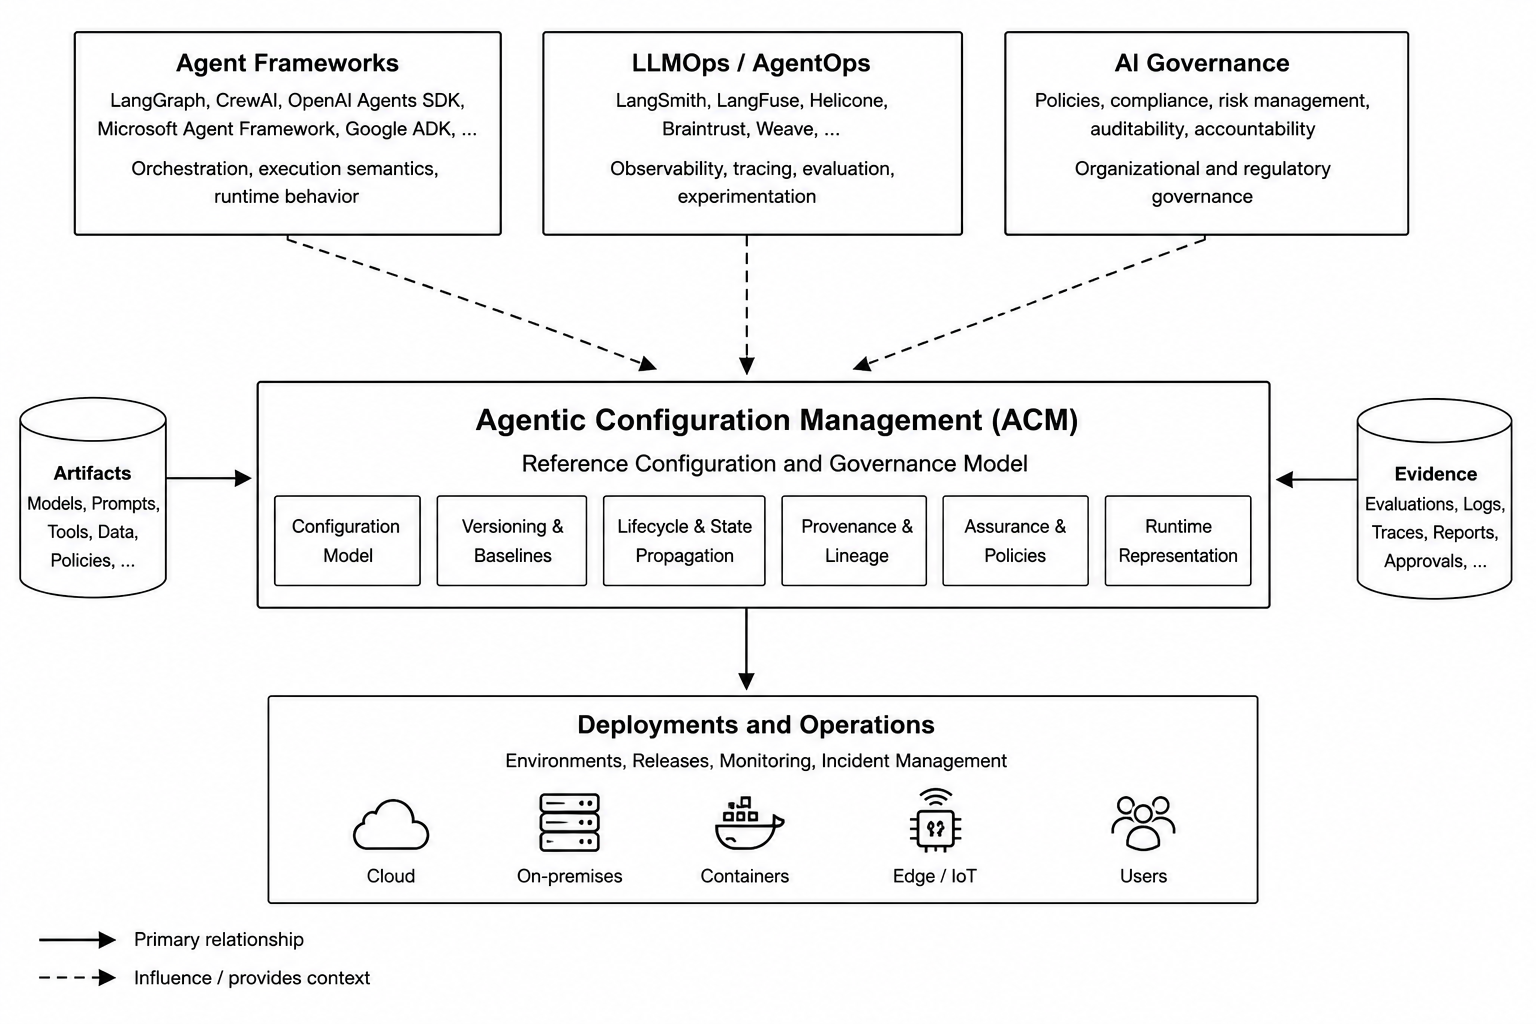
\includegraphics[width=0.7\textwidth]{figures/ACM_architecture_principles.png}
	\caption{Positioning of ACM. ACM acts as a framework-independent configuration layer that connects agent frameworks (orchestration), LLMOps platforms (observability and evaluation) and deployment environments (execution).}
	\label{fig:ACM_positioning}
\end{figure*}

ACM focuses on governing the former while providing formal semantics to interpret the latter relative to the governed configuration. The contributions of this paper are fourfold:

\begin{itemize}
    \item We propose a \textbf{framework-independent governance representation} that defines the core concepts, relationships, and abstractions required to represent governed heterogeneous agentic configurations.
    
    \item We formalize the \textbf{governance semantics} of agentic configurations through lifecycle models, state propagation, assurance semantics, and runtime governance mechanisms.
    
    \item We present a \textbf{reference operationalization} of the model, including a Python reference implementation together with projection mechanisms for heterogeneous agentic frameworks.
    
    \item We evaluate the \textbf{expressiveness and operational feasibility} of the proposed model through normative scenarios, automated validation, quantitative impact analysis and cross-framework projection experiments.
\end{itemize}

The remainder of this paper is organized as follows. Section~\ref{sec:related_work} reviews the foundations of Software Configuration Management, AI governance, LLMOps, AgentOps, and agentic frameworks, and identifies the gap addressed by the Agentic Configuration Model (ACM). Section~\ref{sec:design_principles} derives the design principles of the proposed reference model. Section~\ref{sec:reference_model} introduces the ACM reference model, while Section~\ref{sec:governance_semantics} formalizes its governance semantics. Section~\ref{sec:operationalization} describes its operationalization through a reference architecture, framework adapters, governance algorithms, and a reference implementation. Section~\ref{sec:evaluation} evaluates the proposed model. Finally, Sections~\ref{sec:discussion}, \ref{sec:threats_validity}, \ref{sec:future_work}, and \ref{sec:conclusion} discuss the implications, limitations, future research directions, and conclusions of this work.

\section{Related Work}
\label{sec:related_work}

\subsection{Software Configuration Management}
\label{sec:scm}

Software Configuration Management (SCM) provides the engineering foundations for identifying, controlling, and auditing the evolution of software systems. Rather than focusing solely on version control, SCM defines a disciplined process for establishing configuration baselines, managing change, maintaining traceability, and ensuring that released systems remain reproducible and auditable throughout their lifecycle \cite{whitgift1991methods, conradi1998version, leon2015software, bersoff1984elements, bersoff1978software}.

These principles have been formalized by long-established standards and bodies of knowledge, including IEEE~828, ISO/IEC/IEEE~12207, and the \emph{Software Engineering Body of Knowledge} (SWEBOK) \cite{swebok40, ieee2012ieee, wohlinsnowballing}. Although these references differ in scope, they consistently describe configuration management as a combination of configuration identification, change control, configuration status accounting, and configuration verification and audit.

Classical SCM has proved effective for conventional software systems composed of relatively stable software artifacts such as source code, libraries, documentation, build configurations, and release packages \cite{chacon2014pro}. Its central concepts---configuration items, immutable baselines, controlled revisions, dependency management, and change auditing---provide the foundations required to ensure consistency and reproducibility across software releases.

\begin{figure*}[t]
	\centering
	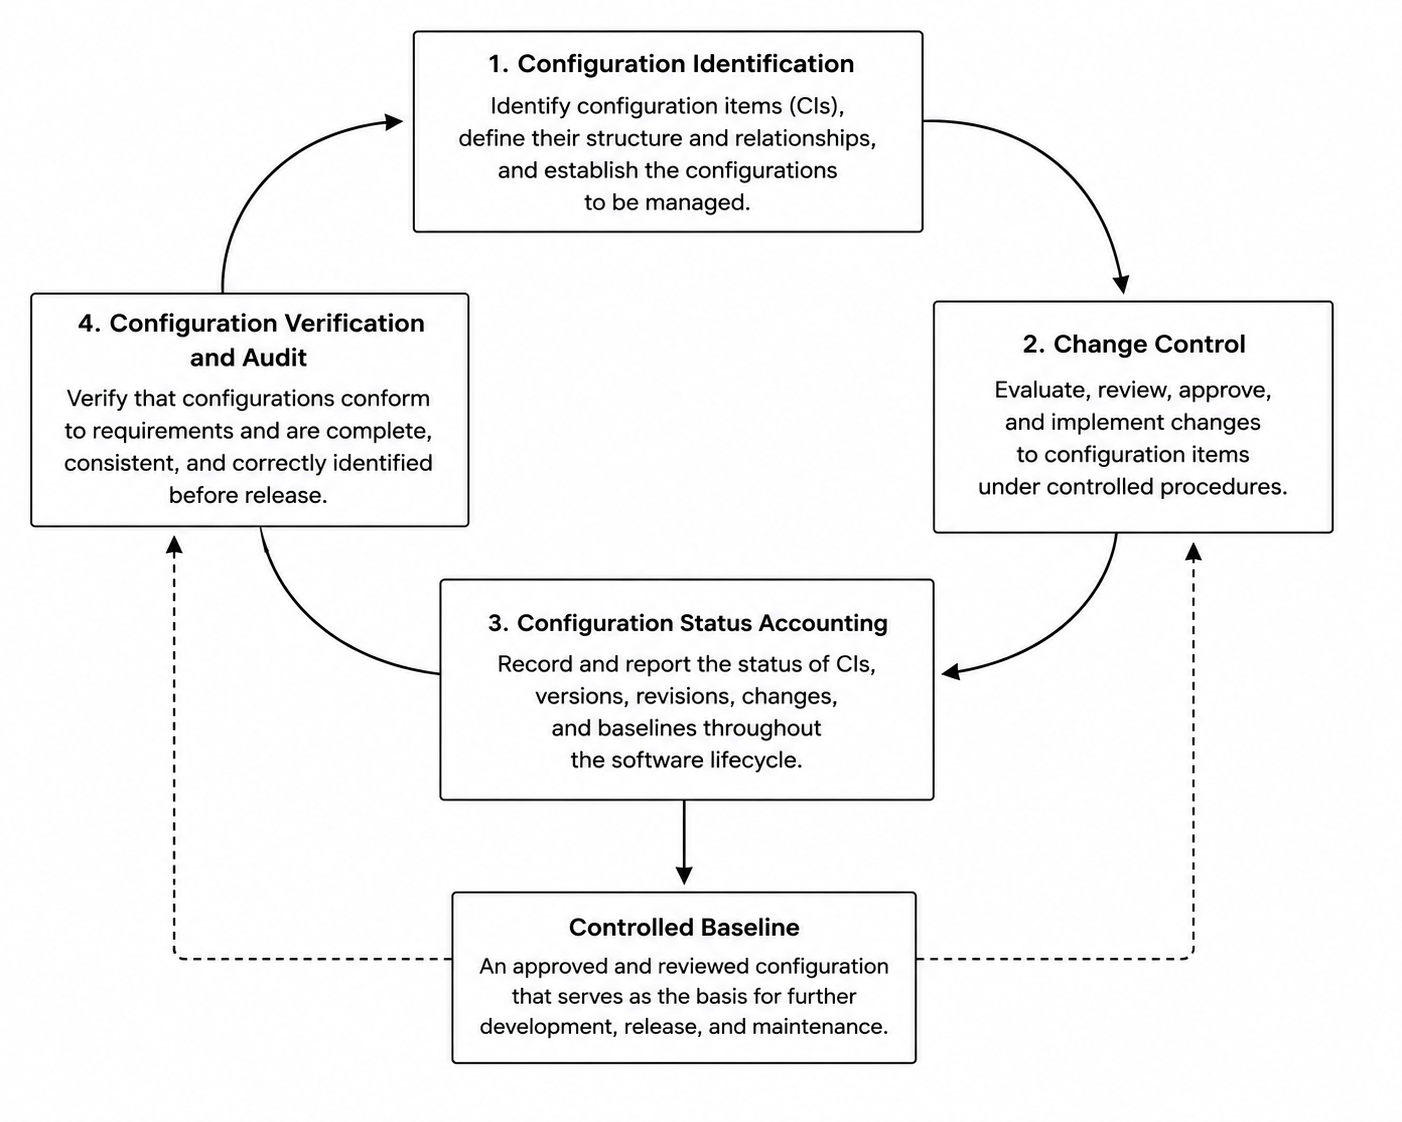
\includegraphics[width=0.7\textwidth]{figures/SCM_configuration_management_liefcycle_baseline.png}
	\caption{Fundamental Software Configuration Management (SCM) process. Configuration identification, change control, configuration status accounting, and configuration verification and audit constitute the four core SCM activities defined by established software engineering standards. Together, they provide the conceptual foundations for immutable revisions, controlled baselines, traceability, and governance that are extended by ACM to heterogeneous agentic systems \cite{bersoff1984elements}.}
	\label{fig:SCM_framework}
\end{figure*}

However, applying these principles directly to agentic systems is not straightforward. In addition to executable software components, agentic systems rely on heterogeneous configurable artifacts, dynamic execution structures, and runtime-generated elements that are not explicitly addressed by traditional SCM models. Consequently, while SCM provides the conceptual foundations for configuration governance, additional abstractions are required to represent and govern the configuration of modern agentic systems.

\subsection{AI Governance}
\label{sec:ai_governance}

The rapid adoption of AI systems has expanded governance concerns beyond traditional software engineering. Recent standards, regulatory frameworks, and technical initiatives emphasize accountability, transparency, risk management, and auditability throughout the AI lifecycle \cite{pandey2025agentic, Engin_Hand_2026, Gangavarapu2025, shavit2023practices, IMDA2026AgenticMGF}. Although these initiatives differ in scope, they share the objective of ensuring that AI systems remain trustworthy, traceable, and subject to appropriate organizational oversight.

From the perspective of agentic systems, three complementary areas are particularly relevant: governance frameworks defining organizational requirements, provenance mechanisms ensuring artifact traceability, and emerging approaches dedicated to the governance of autonomous agents. Together, these perspectives establish important governance objectives but do not define a common configuration representation for heterogeneous agentic systems.

\subsubsection{Governance Frameworks}
\label{sec:governance_frameworks}

Several governance frameworks have established principles for the responsible development and operation of AI systems. Examples include the NIST AI Risk Management Framework (AI RMF), ISO/IEC~42001, ISO/IEC~23894, the OECD AI Principles, and the European AI Act \cite{ai2023artificial, benraouane2024ai, simonetta2024iso, yeung2020recommendation, edwards2021eu}. While their objectives and intended audiences differ, they consistently emphasize governance practices such as accountability, documentation, risk management, human oversight, traceability, and auditability.

These frameworks define organizational objectives and governance processes rather than implementation models. They describe \emph{what} should be governed and documented but intentionally remain independent of the internal representation adopted by AI platforms or execution frameworks. Consequently, they do not provide a framework-independent configuration model capable of representing the complete structure and evolution of an agentic system.

\subsubsection{Provenance and Software Supply Chain}
\label{sec:provenance_supply_chain}

Provenance has become a fundamental requirement for software and AI governance. Existing standards and specifications, including W3C PROV, Software Bills of Materials (SBOMs), SPDX, and the Supply-chain Levels for Software Artifacts (SLSA) \cite{missier2013w3c, SBOM10336262, stewart2010software, okafor2022sok, cobbe2023understanding}, improve traceability by documenting artifact origins, dependencies, integrity, and production processes. These mechanisms strengthen reproducibility, software supply-chain security, and compliance by making software artifacts and their relationships explicitly traceable.

Although highly valuable, these approaches primarily describe software packages, build processes, datasets, or deployment artifacts. They do not represent the semantic configuration of agentic systems, whose behavior depends on heterogeneous configuration artifacts such as agents, prompts, models, skills, composite subsystems, tools, policies, and dynamically evolving execution structures. Consequently, provenance alone is insufficient to govern the configuration of an entire agentic system.

\subsubsection{Governance of Agentic Systems}
\label{sec:agentic_governance}

The emergence of agentic AI has stimulated research on governance mechanisms specifically targeting autonomous and multi-agent systems. Existing approaches typically address runtime supervision, policy enforcement, authorization, monitoring, safety constraints, or operational accountability. Likewise, current AgentOps and orchestration platforms increasingly provide tracing, evaluation, and operational monitoring capabilities for agent execution but are framework-dependent (see Section ~\ref{sec:llmops_agentops}).

This observation complements the limitations identified in classical Software Configuration Management and motivates the need for a unified configuration reference model that separates configuration governance from execution concerns. This gap forms the foundation of the Agentic Configuration Management (ACM) reference model introduced in the following sections.

\subsection{LLMOps and AgentOps}
\label{sec:llmops_agentops}

The emergence of large language models has also given rise to a new generation of operational platforms dedicated to managing AI applications throughout their lifecycle. Inspired by established MLOps practices, LLMOps extends operational support to applications built around foundation models by providing capabilities for prompt management, experimentation, evaluation, deployment, monitoring, and observability. As agentic systems have become increasingly dynamic and autonomous, these practices have naturally evolved toward AgentOps, which addresses the operational management of multi-agent applications and long-running agentic workflows \cite{cesarano2026grand, shavit2023practices, pandey2025agentic, dumas2026}.

Unlike traditional software configuration management, LLMOps and AgentOps focus primarily on the operational lifecycle of AI applications rather than on the governance of their underlying configurations \cite{pahune2025transitioning, amershi2019, dong2024agentops}. Their objective is to facilitate development, deployment, monitoring, experimentation, and continuous improvement while maintaining visibility over system behavior during execution.

Although terminology varies across platforms, most LLMOps and AgentOps solutions converge toward a common set of operational capabilities, including prompt management, execution tracing, evaluation workflows, observability, deployment management, and experiment tracking. These capabilities provide the operational evidence required to understand how an AI application behaves in production and to support iterative improvements of prompts and workflows.

From the perspective of configuration governance, several concepts introduced by these platforms are particularly relevant. 

\begin{itemize}
	\item Configuration management concerns the explicit representation of configurable artifacts and their versions \cite{liu2025towards, Hughes03072025, langfusedocs, heliconedocs}. 
	\item Provenance records the origin and derivation history of these artifacts.
	\item Lineage captures the dependency relationships connecting successive versions, execution traces, and derived artifacts \cite{cesarano2026grand, rajath2025review}. 
	\item Tracing records the sequence of execution events occurring during system operation.
	\item Observability \cite{langsmithdocs} aggregates telemetry that enables operators to inspect the internal behavior of deployed applications \cite{opentelemetry}. 
	\item Deployment state characterizes the operational status of a configuration once deployed within a target environment \cite{braintrustdocs}.
\end{itemize}	

These concepts constitute essential building blocks for governing modern AI applications. However, they generally remain attached to operational artifacts such as prompts, traces, evaluations, or deployments, rather than providing a unified representation of the complete configuration of an agentic system. Relationships among agents, prompts, models, tools, skills, composite subsystems, policies, workflows, and runtime-generated components are typically represented through platform-specific abstractions, preventing the establishment of a framework-independent configuration model.

Representative platforms illustrate this evolution. Prompt management solutions increasingly support prompt versioning, labels, rollback, experimentation, and deployment workflows. Observability platforms provide execution traces, telemetry, evaluation pipelines, and runtime analytics. More recent AgentOps environments extend these capabilities to multi-agent executions through richer runtime monitoring, workflow inspection, and execution replay \cite{sahir2026agentops}. 

As an example of open-source observability platform, we can cite LangFuse~\cite{langfusedocs} providing prompt management, execution tracing, evaluation, experimentation, and prompt versioning. It enables developers to associate prompt revisions with runtime traces, datasets, and evaluation results, thereby improving reproducibility and experimentation across LLM-based applications. 
Another observability platform is Helicone ~\cite{heliconedocs}. It supports request tracing, prompt versioning, experimentation, evaluation, and deployment management. Its primary focus is operational monitoring and prompt-centric development workflows, providing valuable runtime telemetry and performance insights. 

Together, these platforms substantially improve the operational governance of AI applications but remain centered on execution management rather than on the governance of configuration itself, nevertheless they do no aim at representing the complete configuration of heterogeneous agnetic system (see Table ~\ref{tab:llmops_comparison} for a governance capability comparison between the current LLMOPs and AgentOps platforms).

\begin{table*}[t]
\centering
\caption{Representative capabilities of current LLMOps and AgentOps platforms. The comparison highlights their primary focus on operational lifecycle management rather than framework-independent configuration governance.}
\label{tab:llmops_comparison}

\renewcommand{\arraystretch}{1.15}
\begin{tabular}{p{4.2cm}ccccc}
\toprule
\textbf{Capability} &
\textbf{LangSmith} &
\textbf{LangFuse} &
\textbf{Helicone} &
\textbf{Braintrust} &
\textbf{PromptLayer} \\
\midrule

Prompt versioning                & \checkmark & \checkmark & \checkmark & \checkmark & \checkmark \\

Prompt deployment / labels       & $\sim$ & \checkmark & \checkmark & $\sim$ &  \checkmark \\

Execution tracing                & \checkmark & \checkmark & \checkmark & \checkmark & \checkmark \\

Observability / telemetry        & \checkmark & \checkmark & \checkmark & \checkmark & $\sim$ \\

Evaluation workflows             & \checkmark & \checkmark & \checkmark & \checkmark & $\sim$ \\

Experiment tracking              & \checkmark & \checkmark & \checkmark & \checkmark & $\sim$ \\

Prompt provenance                & $\sim$ & \checkmark & \checkmark & $\sim$ & \checkmark \\

Execution lineage                & \checkmark & \checkmark & \checkmark & \checkmark & $\sim$ \\

Deployment state                 & $\sim$ & \checkmark & \checkmark & $\sim$ & \checkmark \\

Runtime replay                   & \checkmark & $\sim$ & $\sim$ & $\sim$ & $\sim$ \\

Framework-specific integrations  & \checkmark & \checkmark & \checkmark & \checkmark & \checkmark \\

\midrule

Framework-independent configuration model
                                 & -- & -- & -- & -- & -- \\

Configuration graph              & -- & -- & -- & -- & -- \\

Immutable configuration baseline & -- & -- & -- & -- & -- \\

Configuration lifecycle          & -- & -- & -- & -- & -- \\

Configuration dependency model   & -- & -- & -- & -- & -- \\

Governed configuration revisions & -- & -- & -- & -- & -- \\

Configuration state propagation  & -- & -- & -- & -- & -- \\

Configuration governance semantics
                                 & -- & -- & -- & -- & -- \\

\bottomrule
\end{tabular}

\vspace{1mm}

\footnotesize
$\checkmark$ Supported \hspace{1em}
$\sim$ Partial support \hspace{1em}
-- Not provided as a first-class capability.

\end{table*}

\subsection{Agentic Frameworks}
\label{sec:agentic_frameworks}

The rapid adoption of agentic AI has led to the emergence of numerous frameworks dedicated to designing and executing autonomous or multi-agent applications. Although their architectures differ, these frameworks share a common objective: orchestrating the execution of agents, coordinating interactions among heterogeneous components, and integrating large language models with external tools, memory, and user-defined workflows (non exhaustive list of frameworks \cite{crewaidocs, langgraphdocs, googleadkdocs, microsoftadkdocs, openaiddocs, claudedocs, mistraldocs}).

Current frameworks cover a broad spectrum of orchestration paradigms. Some adopt explicit graph-based execution models, while others organize applications around agents, tasks, crews, or conversational interactions. Despite these architectural differences, they generally provide abstractions for defining execution flows, invoking tools, managing shared or local state, and coordinating agent interactions during runtime (see Table ~\ref{tab:framework_comparison} in Appendix ~\ref{appendix:related_work}).

Beyond execution, modern frameworks increasingly incorporate operational capabilities such as checkpointing, persistence, human-in-the-loop interactions, execution replay, and integration with observability platforms. These features considerably simplify the development and deployment of agentic applications and complement the operational services provided by LLMOps and AgentOps platforms.

However, the internal representations adopted by these frameworks remain closely coupled to their respective execution models. Configuration artifacts, dependency structures, lifecycle conventions, and runtime abstractions are expressed through framework-specific concepts that are not directly interoperable. Consequently, while these frameworks provide rich execution semantics, they do not define a common representation suitable for governing configurations independently of a particular execution environment.



\subsection{Gap Analysis}
\label{sec:gap_analysis}

The preceding sections have examined complementary perspectives on the governance of AI systems, including Software Configuration Management, AI governance frameworks, LLMOps and AgentOps platforms, and agentic execution frameworks. Although these approaches address different aspects of the AI lifecycle, they collectively contribute to the governance of modern AI applications. However, they cannot simply be combined to obtain a unified configuration-governance solution. Software Configuration Management governs software artifacts but has no framework-independent representation of agentic abstractions. AI governance frameworks define organizational objectives and compliance requirements without specifying a configuration model. LLMOps and AgentOps platforms provide observability, evaluation, and operational tooling, while execution frameworks define runtime semantics through framework-specific abstractions. 

Because each family addresses a different governance concern and relies on its own representation of the system, no common semantic model exists for representing, versioning, and governing heterogeneous agentic configurations independently of their execution environment.
This observation motivates the need for a framework-independent reference configuration model capable of integrating these complementary perspectives while preserving a stable governance representation across heterogeneous agentic ecosystems.

Table~\ref{tab:gap_analysis} synthesizes the coverage of representative governance capabilities across these complementary families of approaches. Rather than comparing the approaches themselves, the analysis evaluates the extent to which each family addresses the governance capabilities required throughout the lifecycle of agentic systems.

\begin{table*}[t]
\centering
\caption{Coverage of representative governance capabilities across complementary families of approaches. A detailed comparison is provided in Appendix Table ~\ref{tab:gap_analysis_detailed}.}
\label{tab:gap_analysis}

\renewcommand{\arraystretch}{1.15}

\begin{tabular}{p{5.2cm}ccccc}
\toprule
\textbf{Governance Capability}
&
\textbf{SCM}
&
\textbf{AI Gov.}
&
\textbf{LLMOps / AgentOps}
&
\textbf{Frameworks}
\\
\midrule

Configuration identification          & \checkmark & $\sim$ & $\sim$ & $\sim$ \\

Version management                    & \checkmark & -- & $\sim$ & $\sim$ \\

Configuration provenance              & $\sim$ & \checkmark & \checkmark & $\sim$ \\

Dependency traceability               & \checkmark & $\sim$ & \checkmark & $\sim$ \\

Execution observability               & -- & $\sim$ & \checkmark & \checkmark \\

Lifecycle governance                  & $\sim$ & \checkmark & $\sim$ & $\sim$ \\

Framework-independent representation  & -- & -- & -- & -- \\

Unified configuration model           & -- & -- & -- & -- \\

\bottomrule
\end{tabular}

\vspace{1mm}

\footnotesize
$\checkmark$ Fully addressed \hspace{1em}
$\sim$ Partially addressed \hspace{1em}
-- Not addressed as a primary capability.

\end{table*}

The limitation of combining these approaches is therefore not the absence of governance, observability, execution, or compliance mechanisms. Rather, these capabilities remain distributed across complementary technologies that operate on different abstractions and representations. As a result, governed configurations cannot be represented, versioned, compared, and evolved through a common semantic model independently of the underlying execution framework. Our reference model ACM addresses this missing abstraction layer by introducing a framework-independent reference configuration model that unifies configuration governance while remaining complementary to existing execution frameworks, LLMOps platforms, AgentOps solutions, and organizational AI governance frameworks. These observations provide the rationale for designing a unified reference model which is presented in the next section. It establishes the requirements for a unified reference model dedicated to configuration governance for agentic systems (see next Section ~\ref{sec:design_principles}).

\section{Design Principles}
\label{sec:design_principles}

Rather than extending an existing orchestration framework or operational platform, the objective of ACM is to establish a reference model that complements these ecosystems while remaining independent of their implementation technologies. ACM addresses therefore a complementary concern by representing governed configurations independently of execution platforms, enabling immutable baselines, dependency-aware configuration management, and explicit relationships between configuration revisions, runtime observations, and assurance evidence.

The design of such a reference model is guided by a set of requirements derived from the limitations identified in the preceding analysis. These principles define the properties that any framework-independent configuration governance model should satisfy. They intentionally describe design requirements rather than implementation choices; the conceptual realization of these principles is introduced in Section~\ref{sec:reference_model}.

Table~\ref{tab:design_principles} summarizes the seven principles that guide the design of ACM.
\begin{table*}[t]
\centering
\caption{Design principles guiding the ACM reference model.}
\label{tab:design_principles}

\renewcommand{\arraystretch}{1.15}

\begin{tabular}{p{1.0cm}p{4.0cm}p{9.2cm}}
\toprule
\textbf{ID} &
\textbf{Principle} &
\textbf{Objective}
\\
\midrule

P1 &
Framework Independence &
Remain independent of execution frameworks, orchestration engines, and AI providers.\\

P2 & Explicit Configuration Representation & Represent every configurable artifact explicitly under configuration governance.\\

P3 &  Immutable Versioning & Ensure deterministic evolution through immutable revisions and controlled baselines. \\

P4 & Configuration–Execution Separation & Clearly distinguish governed configurations from runtime execution.\\

P5 & Explicit Traceability & Preserve provenance and dependency relationships throughout the configuration lifecycle.\\

P6 & Governance by Design & Support lifecycle governance, policy enforcement, assurance, and auditability.\\

P7 & Extensibility & Allow the reference model to evolve without changing its governance foundations.
\\
\bottomrule
\end{tabular}

\end{table*}

\paragraph{P1 -- Framework Independence}

A configuration governance model shall remain independent of any specific orchestration framework, execution engine, or AI provider. Heterogeneous agentic systems should therefore be representable through a common abstraction that preserves governance semantics without exposing framework-specific implementation details. This independence enables interoperability across evolving ecosystems while avoiding dependence on a particular execution technology.

\paragraph{P2 -- Explicit Configuration Representation}

Every artifact whose definition influences the behaviour of an agentic system shall be represented explicitly as a governed configuration object. The model should support heterogeneous artifacts while remaining independent of their implementation and execution semantics.

\paragraph{P3 -- Immutable Versioning}

Configuration evolution shall rely on immutable revisions. Every modification shall produce a new governed revision while preserving previous versions to ensure reproducibility, auditability, and deterministic reconstruction of historical configurations.

\paragraph{P4 -- Configuration--Execution Separation}

Configuration governance shall remain conceptually independent from runtime execution. Runtime observations may enrich governance information but shall not directly modify governed configurations.

\paragraph{P5 -- Explicit Traceability}

The model shall preserve explicit traceability among governed artifacts throughout their lifecycle. Structural dependencies, provenance relationships, and configuration evolution should remain observable and auditable independently of any execution framework.

\paragraph{P6 -- Governance by Design}

Governance shall be an intrinsic property of the configuration model rather than an external operational concern. The model should support lifecycle control, policy evaluation, assurance, auditability, and deterministic governance decisions.

\paragraph{P7 -- Extensibility}

The reference model shall remain extensible to accommodate future categories of configuration artifacts, governance policies, and execution paradigms without modifying its fundamental governance principles.


The following section introduces the ACM reference model, which operationalizes these principles through a normalized representation of governed configuration artifacts and their relationships.

\section{ACM Reference Model}
\label{sec:reference_model}

The ACM is made to offer a common governance layer capable of representing heterogeneous configuration artifacts independently of their execution environment.

The model is designed around three complementary objectives. First, it provides a unified representation of configurable artifacts participating in an agentic system. Second, it explicitly captures the structural and governance relationships among these artifacts. Third, it establishes the conceptual foundations required to support lifecycle management, traceability, provenance, auditability, and configuration evolution.

Section~\ref{sec:conceptual_overview} introduces the conceptual organization of the model. Section~\ref{sec:aci_model} defines the abstract representation of Agentic Configuration Items (ACIs). The following subsections specify the relationships between ACIs, baseline composition, and the structural properties of the reference model.


\subsection{Conceptual Overview}
\label{sec:conceptual_overview}

An agentic system is composed of numerous configurable artifacts originating from heterogeneous technologies, including orchestration frameworks, language models, prompts, tools, skills, composite subsystems, policies, execution environments, and governance mechanisms. Although these artifacts collectively determine the behaviour of the system, they are generally represented through framework-specific abstractions and governed independently.

The ACM reference model introduces a unified conceptual representation in which every configurable artifact is treated as a governed configuration item, regardless of its implementation technology or execution framework. This abstraction enables heterogeneous artifacts to be managed according to a common governance model while preserving their individual semantics.

Rather than organizing configuration items according to implementation technologies, ACM structures them according to the governance role they fulfil within the system. Configuration items are therefore organized into three conceptually independent families:

\begin{itemize}

\item \textbf{Structural items}, which describe the static composition of the system and its configurable artifacts.

\item \textbf{Governance items}, which define policies, assurance evidence, compliance constraints, and lifecycle governance.

\item \textbf{Runtime items}, which represent execution-related information generated during system operation while remaining linked to the governed configuration.

\end{itemize}

Although these families are conceptually independent, they remain connected through explicit relationships that preserve traceability across the complete lifecycle of the system. This organization separates structural configuration, governance information, and runtime observations while allowing each perspective to evolve independently.

To represent these complementary perspectives, ACM organizes configuration information into four interconnected conceptual graphs, illustrated in Figure~\ref{fig:acm_reference_model}.

\begin{itemize}

\item The \textbf{Configuration Graph} represents the governed configuration of the agentic system and the structural relationships among configuration items.

\item The \textbf{Assurance Graph} captures governance policies, assurance evidence, compliance constraints, and policy enforcement.

\item The \textbf{Runtime Graph} represents execution observations generated during system operation while maintaining explicit links to governed configuration items.

\item The \textbf{Evolution Graph} provides an integrated view of configuration evolution and history from a baseline.

\end{itemize}

The decomposition into four complementary graphs is a deliberate design decision rather than a modeling convenience. Each graph addresses a distinct governance concern that follows its own semantics and lifecycle. Separating these orthogonal concerns preserves conceptual clarity, avoids mixing static and dynamic governance information, and enables each graph to evolve independently while remaining linked through explicit traceability relationships. 

\begin{figure*}[t]
	\centering
	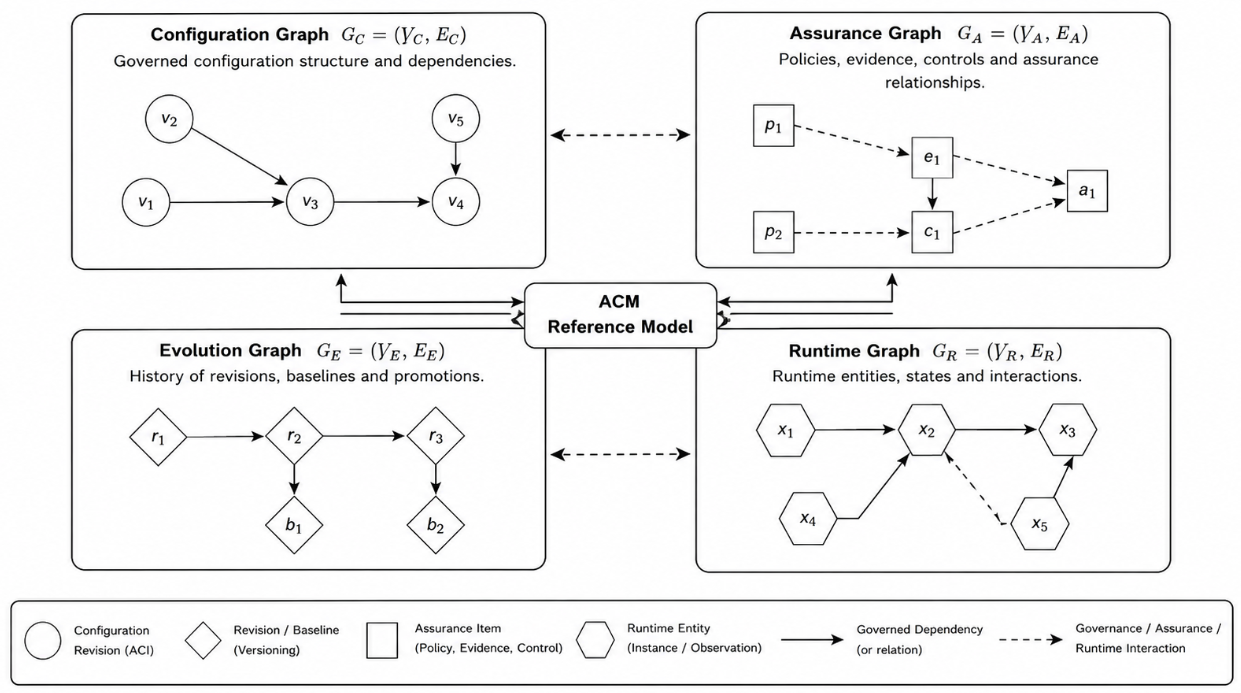
\includegraphics[width=0.6\textwidth]{figures/ACM_reference_model.png}
	\caption{Multi-graph organization of the ACM reference model. Configuration, evolution, runtime, and assurance are represented as four complementary governance views that share the same immutable configuration revisions. This separation allows each graph to evolve according to its own semantics while maintaining explicit consistency and traceability through a common revision space.}
	\label{fig:acm_reference_model}
\end{figure*}

\subsection{Agentic Configuration Item}
\label{sec:aci_model}

The Agentic Configuration Item (ACI) is the fundamental abstraction of the ACM reference model. An ACI represents any configurable artifact whose definition contributes to the specification, governance, or execution of an agentic system. By introducing a common abstraction independent of implementation technologies, ACM enables heterogeneous artifacts originating from different frameworks to be represented and governed uniformly.

Unlike traditional software configuration items, which primarily describe software artifacts, ACIs encompass the broader range of configurable elements required by modern agentic systems. Examples include agents, prompts, skills, composite subsystems, workflows, tools, language models, policies, assurance evidence, runtime observations, and other governance artifacts. Although these artifacts differ in purpose and lifecycle, they share a common representation within the ACM reference model (see Figure ~\ref{fig:aci_metamodel}).

Every ACI is represented as an immutable configuration revision. Once created, the content associated with a revision never changes; any modification results in the creation of a new revision while preserving previous versions for reproducibility, auditability, and deterministic reconstruction of historical configurations. Configuration evolution is therefore represented explicitly through successive governed revisions rather than mutable objects.

An ACI combines three complementary dimensions:

\begin{itemize}

\item an immutable configuration content describing the governed artifact;

\item an identity and revision model ensuring uniqueness, version management, and reproducibility;

\item governance metadata describing lifecycle information, provenance, integrity, and other management attributes required for configuration governance.

\end{itemize}

This representation intentionally separates the conceptual identity of a configuration item from the successive revisions describing its evolution. A configuration item therefore exists independently of any particular revision, while each revision represents a complete immutable state of that item at a specific point in its lifecycle.

To accommodate the diversity of configurable artifacts encountered in agentic systems, ACIs are organized into three conceptually independent families introduced in Section~\ref{sec:conceptual_overview}: Structural ACIs, Governance ACIs, and Runtime ACIs. These families share the same abstract representation while specializing the governed content according to the role performed by each artifact within the reference model. This specialization enables the model to remain extensible without introducing family-specific governance mechanisms.

Figure~\ref{fig:aci_metamodel} presents the abstract representation of an Agentic Configuration Item. The following subsections specify its attributes, relationships, and composition rules.

\begin{figure*}[t]
	\centering
	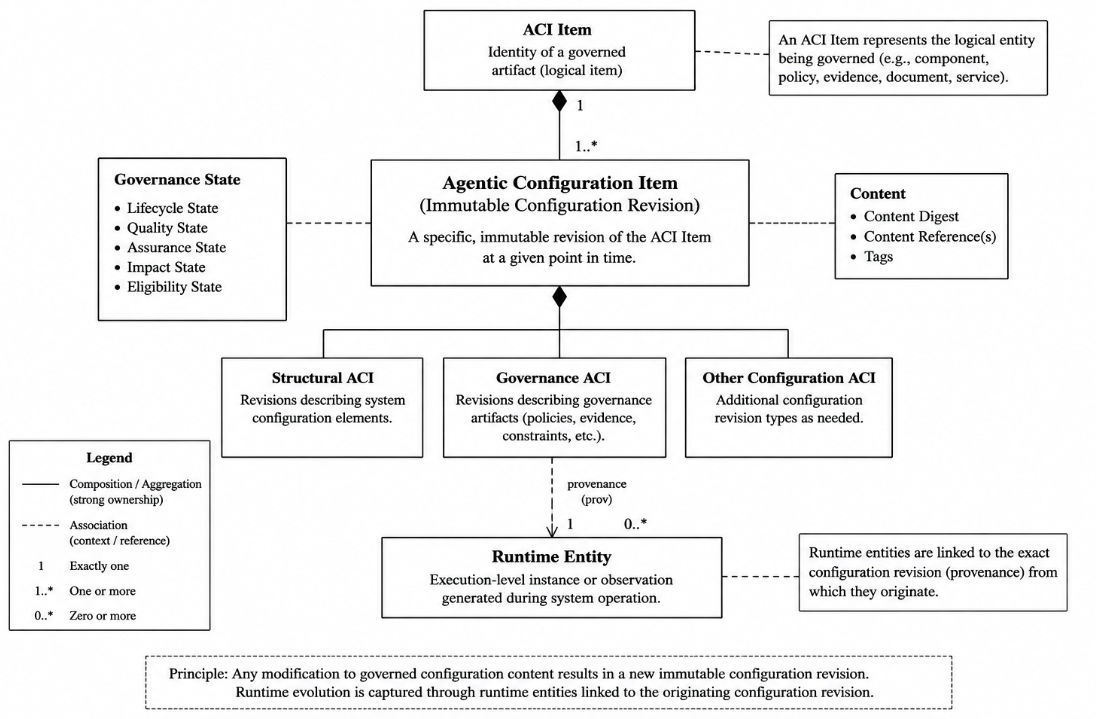
\includegraphics[width=\textwidth]{figures/ACI_metamodel_old.png}
	\caption{Metamodel of the Agentic Configuration Item (ACI). The ACI constitutes the fundamental building block of the ACM reference model. The metamodel defines a common representation for governed configuration items, their specialization hierarchy (Structural, Governance, and Runtime ACIs), agentic configuration types, and governance metadata. Associated entities, including provenance records, content digests, content references, and tags, provide the information required for immutable identification, traceability, integrity verification, and reproducible configuration management.}
	\label{fig:aci_metamodel}
\end{figure*}

\subsection{ACI Representation}
\label{sec:configuration_item_representation}

The abstract representation introduced in the previous section is realized through a normalized set of attributes shared by all Agentic Configuration Items, regardless of their specialization. This common representation provides a consistent governance model while allowing individual artifact categories to define their own domain-specific content.

The representation of an ACI is organized into four complementary components:

\begin{itemize}

\item \textbf{Identity}, uniquely identifying both the configuration item and the immutable revision to which the representation corresponds.

\item \textbf{Governance state}, describing the lifecycle, quality, compliance, and assurance status associated with the revision.

\item \textbf{Configuration content}, containing the governed artifact together with integrity information and extensible metadata.

\item \textbf{Governance metadata}, recording provenance, user-defined properties, and additional information required for lifecycle management and auditing.

\end{itemize}

This separation isolates the immutable content of a configuration revision from the metadata required to govern its evolution. Consequently, governance information may evolve independently from the business semantics of individual artifact categories while preserving the integrity of immutable revisions.

Table~\ref{tab:aci_attributes} summarizes the attributes composing the abstract representation of an ACI.

\begin{table*}[t]
\centering
\caption{Abstract attributes of an Agentic Configuration Item revision.}
\label{tab:aci_attributes}

\renewcommand{\arraystretch}{1.15}

\begin{tabular}{p{3.3cm}p{3.4cm}p{8.3cm}}

\toprule

\textbf{Category} &
\textbf{Representative Attributes} &
\textbf{Purpose}

\\
\midrule

Identity &
item\_id, revision\_id &
Uniquely identify the governed item and its immutable revision.

\\

Governance State &
lifecycle\_state, quality\_state, assurance\_state, compliance\_state &
Describe the governance status of the revision.

\\

Configuration Content &
content, digest, metadata &
Represent the governed artifact together with integrity and extensible descriptive information.

\\

Governance Metadata &
provenance, tags, custom properties &
Support traceability, auditing, provenance, and organization-specific extensions.

\\

\bottomrule

\end{tabular}

\end{table*}

Although every ACI shares this common representation, the interpretation of the governed content depends on the specialization of the configuration item. Structural, Governance, and Runtime ACIs therefore reuse the same abstract representation while encapsulating different categories of governed artifacts.

\subsection{Relationship Model}
\label{sec:configuration_relationships}

Individual configuration items do not exist in isolation. The complete configuration of an agentic system emerges from the explicit relationships connecting governed artifacts across structural, governance, and runtime perspectives. These relationships constitute the semantic backbone of the ACM reference model by preserving dependency information independently of any execution framework.

Unlike conventional orchestration frameworks, where relationships are often embedded within implementation-specific structures, ACM represents relationships as explicit governed entities. This representation enables dependency analysis, impact assessment, provenance tracking, and configuration validation to be performed independently of execution technologies.

ACM distinguishes several categories of relationships according to their governance semantics:

\begin{itemize}

\item \textbf{Configuration relationships} describe the composition and dependency structure of governed configuration items.

\item \textbf{Assurance relationships} associate configuration items with policies, assurance evidence, compliance requirements and ownership.

\item \textbf{Runtime relationships} connect execution observations to the governed configuration from which they originate.

\item \textbf{Evolution relationships} preserve provenance, revision lineage, and derivation history.

\end{itemize}

Each relationship is explicitly typed and directional. Relationship types define their admissible source and target configuration items together with the semantic constraints governing their interpretation. This explicit typing allows validation rules to be evaluated independently from artifact implementations while ensuring consistent dependency semantics across heterogeneous agentic systems.

Figure~\ref{fig:relationship_model} illustrates the conceptual organization of relationship categories within the ACM reference model.
\begin{figure*}[t]
	\centering
	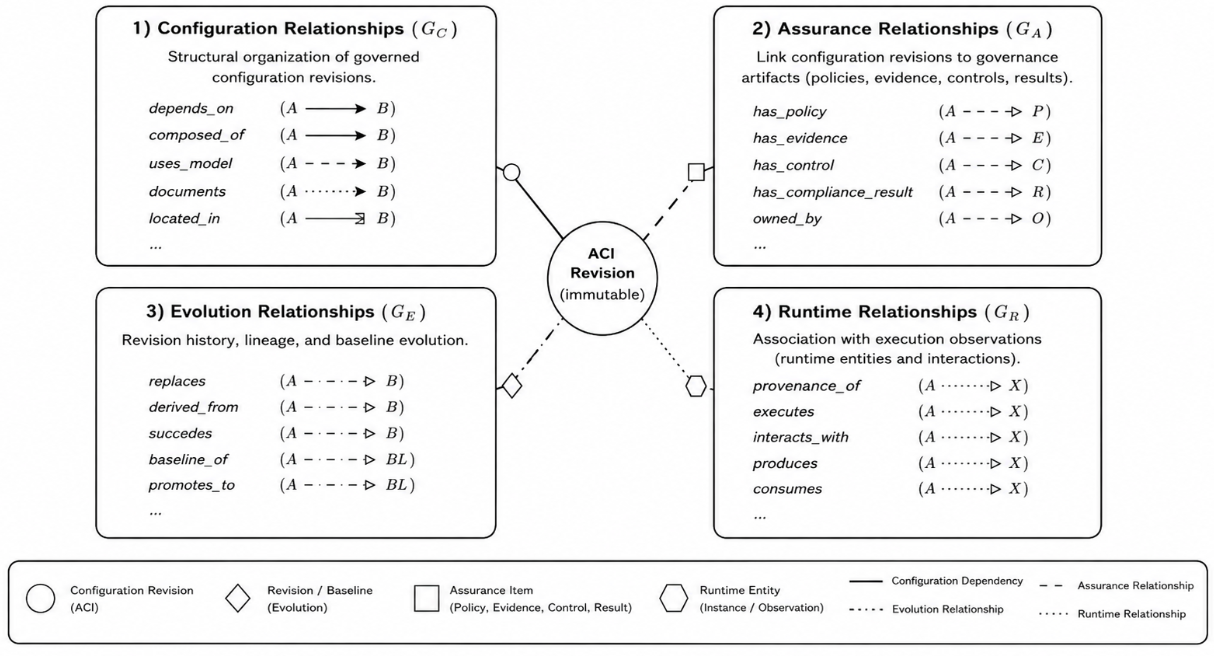
\includegraphics[width=0.6\textwidth]{figures/aci_relationship.png}
	\caption{Relationship categories associated with an immutable \textit{ACI Revision}. ACM organizes relationships into four complementary families aligned with the governance views of the reference model. Configuration relationships describe the structural organization of governed configuration items, Evolution relationships capture revision history and baseline evolution, Runtime relationships associate immutable revisions with execution observations, and Assurance relationships link configuration revisions to governance evidence, compliance results, and policy enforcement. This categorization separates orthogonal governance concerns while preserving explicit traceability through a common immutable revision.}
	\label{fig:relationship_model}
\end{figure*}

\subsection{Release Baselines}
\label{sec:release_baselines}

While Agentic Configuration Items represent individual governed artifacts, operational deployments require a consistent representation of complete system configurations. ACM introduces the notion of a \emph{Release Baseline} to capture a coherent and reproducible snapshot of an agentic system at a specific point in its evolution.

A Release Baseline is an immutable collection of ACI revisions that collectively define the governed configuration of an agentic system. Rather than referencing configuration items independently of their evolution, a baseline always references specific immutable revisions, ensuring that the complete configuration can be reconstructed \emph{deterministically} at any time.

The purpose of a Release Baseline extends beyond simple version aggregation. It establishes the governance boundary within which configuration consistency, traceability, compliance, and assurance can be evaluated. Consequently, governance decisions are performed on complete configurations rather than on isolated artifacts whenever system-wide consistency is required.

A Release Baseline is characterized by the following properties:

\begin{itemize}

\item it references immutable revisions rather than mutable configuration items;

\item it represents a complete and internally consistent governed configuration;

\item it preserves all structural, governance, runtime, and traceability relationships among referenced artifacts;

\item it constitutes the primary unit for reproducibility, audit, release management, and compliance assessment.

\end{itemize}

Baselines are themselves governed configuration objects. They possess their own identity, lifecycle, provenance, and governance metadata while remaining immutable after publication. The evolution of a system is therefore represented as a sequence of immutable Release Baselines, each corresponding to a governed configuration state.

Because every baseline references immutable ACI revisions, historical configurations remain reproducible even when individual configuration items continue to evolve. This property enables deterministic reconstruction, historical audits, rollback, and longitudinal analysis without modifying previously released configurations.

Figure~\ref{fig:release_baseline} illustrates the conceptual organization of a Release Baseline and its relationship with the governed configuration items composing an agentic system.
\begin{figure*}[t]
	\centering
	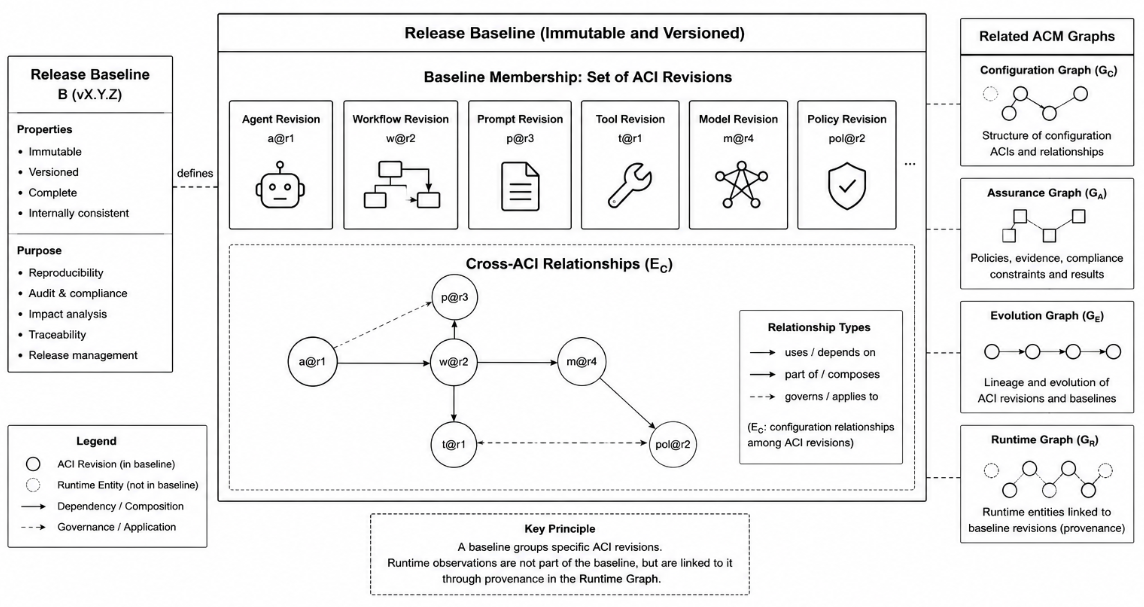
\includegraphics[width=\textwidth]{figures/release_baseline.png}
	\caption{Conceptual organization of an ACM release baseline. A release baseline defines an immutable and versioned snapshot of the governed configuration by grouping a consistent set of ACI revisions. Baseline membership explicitly identifies the configuration revisions composing the release, while cross-ACI relationships preserve the structural dependencies among configuration items (e.g., agents, workflows, prompts, tools, models, and policies). This separation allows a baseline to provide a reproducible configuration snapshot while maintaining the dependency information required for impact analysis, traceability, and governance throughout the system lifecycle.}
	\label{fig:release_baseline}
\end{figure*}

\section{Governance Semantics}
\label{sec:governance_semantics}

The ACM reference model specifies the structural organization of governed agentic systems. This section complements the metamodel by defining the operational semantics governing lifecycle evolution, state evaluation, dependency propagation, and runtime reconstruction.

The governance semantics are intentionally defined independently from any execution framework. Their purpose is not to describe execution behavior but to provide a deterministic interpretation of governed configurations throughout their lifecycle.

Let

\begin{equation}
	G=(V,E)
	\label{eq:configuration_graph}
\end{equation}

denote the ACM Configuration Graph introduced in Section~\ref{sec:configuration_graph}, where each vertex represents an immutable ACI revision and each edge represents a typed governance relationship.

Each revision is associated with a governance descriptor

\begin{equation}
	\Gamma(v)=
	\left(
	L(v),
	Q(v),
	A(v),
	I(v),
	El(v),
	Rt(v)
	\right),
	\label{eq:governance_descriptor}
\end{equation}

where the individual components respectively denote the lifecycle, quality, assurance, impact, eligibility, and runtime states associated with revision $v$.

The governance descriptor is a logical representation of the governance status of an ACI revision. It does not perform any computation itself. Individual state components are evaluated independently according to the semantics introduced in the following subsections and are subsequently propagated through governance relationships according to explicitly defined propagation policies.

This separation between state spaces, evaluation functions, propagation policies, and runtime reconstruction ensures that each semantic component is defined once and reused consistently throughout the model.

\subsection{Governance Lifecycle}
\label{sec:lifecycle_semantics}

The lifecycle dimension represents the intrinsic governance maturity of an immutable ACI revision independently of any dependency or runtime consideration. Unlike the remaining governance dimensions, lifecycle states are explicitly assigned through governance actions rather than derived by propagation.

Figure~\ref{fig:lifecycle_state_machine} presents the lifecycle state machine associated with every ACI revision.

Each revision progresses monotonically through the lifecycle. Once a revision reaches a given state, it cannot transition back to a previous lifecycle state.

This monotonic property guarantees configuration immutability while preserving complete governance traceability across successive revisions.

Lifecycle transitions are therefore constrained by a partial order

\begin{equation}
	Draft
	<
	Validated
	<
	Approved
	<
	Released
	<
	Deprecated
	<
	Archived,
	\label{eq:lifecycle_order}
\end{equation}

where each transition represents an explicit governance decision.

The lifecycle state is denoted

\begin{equation}
	L(v)\in\mathcal{L},
	\label{eq:lifecycle_state}
\end{equation}

where $\mathcal{L}$ denotes the lifecycle state space formally defined in Appendix~\ref{appendix:lifecycle}.

Unlike derived governance dimensions introduced later in this section, lifecycle states never result from dependency propagation. They constitute primary governance information from which eligibility and propagation decisions are subsequently derived.

\subsection{Governance State Spaces}
\label{sec:governance_state_spaces}

The governance semantics are defined over six orthogonal state spaces describing complementary aspects of an immutable ACI revision. Each state space captures an independent governance concern and is evaluated according to its own semantics.

Unlike the lifecycle state, which is explicitly assigned through governance decisions, the remaining dimensions are either derived from governance evidence, dependency analysis, or runtime observations.

Figure~\ref{fig:governance_state_machine} summarizes the six orthogonal state machines used throughout the remainder of this paper.

The governance dimensions are:

\begin{itemize}
	\item \textbf{Lifecycle ($\mathcal{L}$):} governance maturity of a revision;
	\item \textbf{Quality ($\mathcal{Q}$):} validation status of the revision itself;
	\item \textbf{Assurance ($\mathcal{A}$):} completeness of governance evidence;
	\item \textbf{Impact ($\mathcal{I}$):} propagation status resulting from dependency analysis;
	\item \textbf{Eligibility ($\mathcal{E}$):} authorization for operational use;
	\item \textbf{Runtime ($\mathcal{R}$):} observed execution state.
\end{itemize}

Each state space is formally defined in Appendix~\ref{appendix:state_spaces}. Their interaction is specified later through evaluation functions and the propagation operator.

\subsection{Propagation Policies}
\label{sec:propagation_policies}

Governance propagation is intentionally separated from state evaluation. While governance state spaces define \emph{what} is evaluated, propagation policies define \emph{how} governance information is allowed to traverse configuration relationships.

Each relationship type is therefore associated with a propagation policy determining the effect of governance changes on dependent revisions. Policies are intrinsic properties of relationship types and remain independent of the current governance states of the connected revisions.

A propagation policy is defined as a mapping

\begin{equation}
	\Pi : T_R \rightarrow \mathcal{P},
	\label{eq:policy_mapping}
\end{equation}

where $T_R$ denotes the set of relationship types introduced by the reference model and $\mathcal{P}$ is the finite set of propagation policies

\begin{equation}
	\mathcal{P}=
	\left\{
	\textit{Blocking},
	\textit{Warning},
	\textit{Informational},
	\textit{None}
	\right\}.
	\label{eq:policy_space}
\end{equation}

Each policy specifies the governance significance of a relationship during propagation.

\begin{itemize}
	\item \textbf{Blocking} indicates that governance changes affecting the source revision shall propagate to dependent revisions and may restrict their operational eligibility until reassessment is completed.
	
	\item \textbf{Warning} propagates governance information without automatically preventing operational use. The affected revision remains executable but requires governance attention.
	
	\item \textbf{Informational} records the dependency for traceability purposes without modifying governance states.
	
	\item \textbf{None} disables propagation across the relationship while preserving the structural dependency.
\end{itemize}

Propagation policies are associated with relationship types rather than individual revisions. Consequently, identical relationship types always induce identical propagation semantics independently of the connected ACI revisions.

When several propagation paths converge on the same revision, multiple propagation policies may simultaneously apply. Their combined effect is resolved deterministically according to the precedence rules defined in Appendix~\ref{appendix:propagation_policies}. This deterministic composition guarantees that governance propagation remains independent of traversal order.

\subsection{Governance Evaluation Functions}
\label{sec:evaluation_functions}

The governance state spaces introduced previously define the possible states associated with an ACI revision. Governance evaluation functions determine how these states are assigned from governance evidence while remaining independent of dependency propagation.

Three evaluation functions are defined. They respectively evaluate intrinsic quality, governance assurance, and operational eligibility. Each function produces a deterministic result for a given governance context and is evaluated independently before any propagation mechanism is applied.

\subsubsection{Quality Evaluation}

The quality evaluation function assigns the quality state associated with an ACI revision according to the available validation evidence.

\begin{equation}
	f_{\mathrm{quality}} : V \rightarrow \mathcal{Q},
	\label{eq:f_quality}
\end{equation}

where $V$ denotes the set of ACI revisions and $\mathcal{Q}$ is the quality state space introduced in Section~\ref{sec:governance_state_spaces}.

The resulting quality state is denoted

\begin{equation}
	Q(v)=f_{\mathrm{quality}}(v).
	\label{eq:quality_assignment}
\end{equation}

Quality evaluation depends exclusively on the considered revision and is therefore independent of dependency propagation.

\subsubsection{Assurance Evaluation}

The assurance evaluation function determines the completeness of governance evidence associated with a revision.

\begin{equation}
	f_{\mathrm{assurance}} : V \rightarrow \mathcal{A},
	\label{eq:f_assurance}
\end{equation}

where $\mathcal{A}$ denotes the assurance state space.

The resulting assurance state is

\begin{equation}
	A(v)=f_{\mathrm{assurance}}(v).
	\label{eq:assurance_assignment}
\end{equation}

Assurance reflects the completeness of governance evidence independently of the intrinsic quality of the revision.

\subsubsection{Eligibility Evaluation}

Operational eligibility depends on the combined interpretation of the governance dimensions. Unlike quality and assurance, eligibility is therefore derived from multiple governance states.

The eligibility evaluation function is defined as

\begin{equation}
	f_{\mathrm{elig}} :
	\mathcal{L}
	\times
	\mathcal{Q}
	\times
	\mathcal{A}
	\times
	\mathcal{I}
	\times
	\mathcal{P}
	\rightarrow
	\mathcal{E},
	\label{eq:f_elig}
\end{equation}

where $\mathcal{P}$ denotes the propagation policy space defined in Section~\ref{sec:propagation_policies}.

The eligibility state associated with revision $v$ is therefore

\begin{equation}
	El(v)=
	f_{\mathrm{elig}}
	\left(
	L(v),
	Q(v),
	A(v),
	I(v),
	\Pi
	\right).
	\label{eq:eligibility_assignment}
\end{equation}

Eligibility summarizes the governance status required for operational use. The evaluation itself remains local to the considered revision. Dependency propagation and the computation of effective governance states are introduced separately in the following subsection.

\subsection{Propagation Semantics}
\label{subsec:propagation_semantics}

The governance dimensions introduced in the previous subsections define the
local state associated with each ACI revision. Governance evaluation, however,
cannot be performed independently for each revision because configuration
dependencies may propagate the consequences of a local change throughout the
configuration graph. The propagation semantics therefore define how governance
states are iteratively updated until a globally consistent evaluation is
reached.

Propagation follows the directed relationships of the configuration graph and
is controlled by the propagation policies introduced in
Section~\ref{subsec:propagation_policies}. These policies determine whether a
relationship blocks propagation, propagates a warning, carries informational
effects only, or does not participate in governance propagation.

The propagation process is defined by a global operator,
denoted $\mathrm{Prop}$, which applies the propagation policies over the
configuration graph and updates the impact state of affected revisions.
Evaluation functions introduced in the previous subsection are subsequently
applied locally to derive the resulting governance states.

Formally, let

\begin{equation}
	\label{eq:prop_operator}
	\mathrm{Prop} :
	G \times \Pi
	\rightarrow
	G,
\end{equation}

where $G$ denotes the governed configuration graph and $\Pi$ the propagation
policy associated with each relationship type.

Starting from an initial governance state, successive applications of
$\mathrm{Prop}$ generate the sequence

\begin{equation}
	\label{eq:prop_iteration}
	G^{(k+1)}
	=
	\mathrm{Prop}
	\!\left(
	G^{(k)},
	\Pi
	\right),
\end{equation}

where $k$ denotes the propagation iteration.

Propagation terminates when the governance state becomes stable, that is, when
an additional application of the operator no longer modifies any propagated
state.

\begin{equation}
	\label{eq:fixed_point}
	\mathrm{Prop}
	\!\left(
	G^{*},
	\Pi
	\right)
	=
	G^{*}.
\end{equation}

The resulting graph $G^{*}$ is called the \emph{least fixed point} of the
propagation semantics and represents the unique governance state used by the
subsequent runtime evaluation.

Because impact propagation is performed before eligibility evaluation,
the eligibility of each revision remains a purely local computation.
Once the propagated impact state has stabilized, the eligibility state is
obtained by applying the evaluation function defined in
Section~\ref{subsec:governance_evaluation} to the final governance descriptor
associated with each revision.

The propagation semantics are independent of any implementation strategy.
A compliant implementation may therefore employ different execution algorithms,
provided that they compute the same least fixed point. The reference
implementation adopts a worklist-based evaluation strategy because it avoids
re-evaluating unaffected revisions while preserving the normative semantics.
The complete worklist algorithm, together with the proofs of monotonicity,
termination, convergence, and uniqueness of the least fixed point, is provided
in Appendix~A.5.







%%%%%%%%%%%%%%%%%%%%%%%%%%%%%%%%%%%%%%%%%%%%%%%%%%%%%%%%%%%%%%%%%%%%%%%%%%%%%%%%
\subsubsection{Impact State Machine}

Configuration modifications rarely affect only one component.
A change introduced into one ACI may invalidate downstream configurations,
runtime deployments, validation evidence, or governance approvals.

To capture these dependencies, ACM introduces an impact propagation state
machine.

Its state space is

\begin{equation}
\mathcal{I}
=
\{
None,
Local,
Propagated
\}.
\label{eq:impact_state}
\end{equation}

with mapping

\begin{equation}
I
:
V
\rightarrow
\mathcal{I}.
\label{eq:mapping_impact_state}
\end{equation}

Impact transitions are generated by dependency propagation algorithms
introduced later in Section~\ref{subsec:impact_semantics}.

Unlike governance quality, impact states are entirely computed.
They are never assigned manually.

For every dependency edge

\begin{equation}
(u,v)\in E,
\label{eq:uv_definition}
\end{equation}

an update of

\begin{equation}
u
\label{eq:u_definition}
\end{equation}

may trigger

\begin{equation}
I(v)=Propagated.
\label{eq:uv_propagation}
\end{equation}

The corresponding propagation semantics are formally defined in
Section~\ref{subsec:impact_semantics}.

%%%%%%%%%%%%%%%%%%%%%%%%%%%%%%%%%%%%%%%%%%%%%%%%%%%%%%%%%%%%%%%%%%%%%%%%%%%%%%%%
\subsubsection{Assurance State Machine}

Governance decisions frequently depend not only on configuration correctness
but also on available evidence demonstrating that required validation
activities have been successfully completed.

ACM therefore distinguishes governance quality from governance assurance.

The assurance state space is

\begin{equation}
\mathcal{A}
=
\{
Unassessed,
Partial,
Satisfied
\}.
\label{eq:assurance_state}
\end{equation}

with

\begin{equation}
A
:
V
\rightarrow
\mathcal{A}.
\label{eq:assurance_state_function}
\end{equation}

Transitions depend on the evaluation of governance evidence such as

\begin{itemize}
    \item executed validation procedures,
    \item benchmark results,
    \item human approvals,
    \item compliance reports,
    \item dependency assurance.
\end{itemize}

Unlike quality states, assurance evaluation is monotonic only while the
governance context remains unchanged.
Whenever configuration dependencies evolve, assurance may legitimately return
to the \emph{Partial} or \emph{Unassessed} state.

This distinction prevents obsolete validation evidence from being considered
valid after significant configuration modifications.

%%%%%%%%%%%%%%%%%%%%%%%%%%%%%%%%%%%%%%%%%%%%%%%%%%%%%%%%%%%%%%%%%%%%%%%%%%%%%%%%
\subsubsection{Execution Eligibility State Machine}

Operational deployment decisions should not depend on a single governance
criterion.

Instead, ACM computes execution authorization by combining lifecycle maturity,
governance quality, impact propagation and assurance evaluation.

The eligibility state is then computed by a deterministic evaluation function combining the lifecycle, quality, assurance, and impact states associated with the revision:

\begin{equation}
	\label{eq:eligibility_function}
	f_{\mathrm{elig}}
	:
	\mathcal{L}
	\times
	\mathcal{Q}
	\times
	\mathcal{A}
	\times
	\mathcal{I}
	\rightarrow
	\mathcal{E},
\end{equation}

where $\mathcal{E}$ denotes the eligibility state space.

with mapping

\begin{equation}
E
:
V
\rightarrow
\mathcal{E}.
\label{eq:eligibility_state_mapping}
\end{equation}

The eligibility of an individual revision is then obtained by applying the
evaluation function to its local governance state.

\begin{equation}
	\label{eq:eligibility_definition}
	El(v)
	=
	f_{\mathrm{elig}}
	\bigl(
	L(v),
	Q(v),
	A(v),
	I(v)
	\bigr)
\end{equation}

The resulting eligibility state is subsequently used by the propagation semantics
defined in the next subsection.

%The formal definition of

%\[
%f
%\]

%is introduced in
%Section~\ref{subsec:eligibility}.

Separating eligibility from the remaining governance dimensions ensures that
authorization policies can evolve independently from lifecycle management or
validation mechanisms.



%%%%%%%%%%%%%%%%%%%%%%%%%%%%%%%%%%%%%%%%%%%%%%%%%%%%%%%%%%%%%%%%%%%%%%%%%%%%%%%%
\subsubsection{Global Governance Vector}

Combining the previous state machines yields the governance descriptor

\begin{equation}
\Gamma(v)
=
(
L_v,
Q_v,
A_v,
I_v,
E_v
),
\label{eq:governance_vector}
\end{equation}

which constitutes the complete semantic representation of an ACI revision.

Lifecycle defines governance maturity.

Quality evaluates intrinsic correctness.

Impact captures dependency propagation.

Assurance measures validation evidence.

Eligibility determines operational authorization.

Each component evolves according to its own semantics while remaining
mathematically independent.

%%%%%%%%%%%%%%%%%%%%%%%%%%%%%%%%%%%%%%%%%%%%%%%%%%%%%%%%%%%%%%%%%%%%%%%%%%%%%%%%
\subsubsection{Unified Governance State Diagram}

Figure~\ref{fig:governance_state_machine} illustrates the interaction between
the lifecycle state and the four orthogonal governance state machines.

%===============================================================================
% TikZ placeholder
%
% The figure shall represent:
%
% - Lifecycle chain:
%   Draft -> Review -> Validated -> Approved -> Deprecated -> Archived
%
% - Four independent state machines:
%     Quality
%     Impact
%     Assurance
%     Eligibility
%
% - Evaluation function:
%
%      (L,Q,A,I) ---> Eligibility
%
% IEEE academic style.
%
%===============================================================================

\begin{figure*}[t]
	\centering
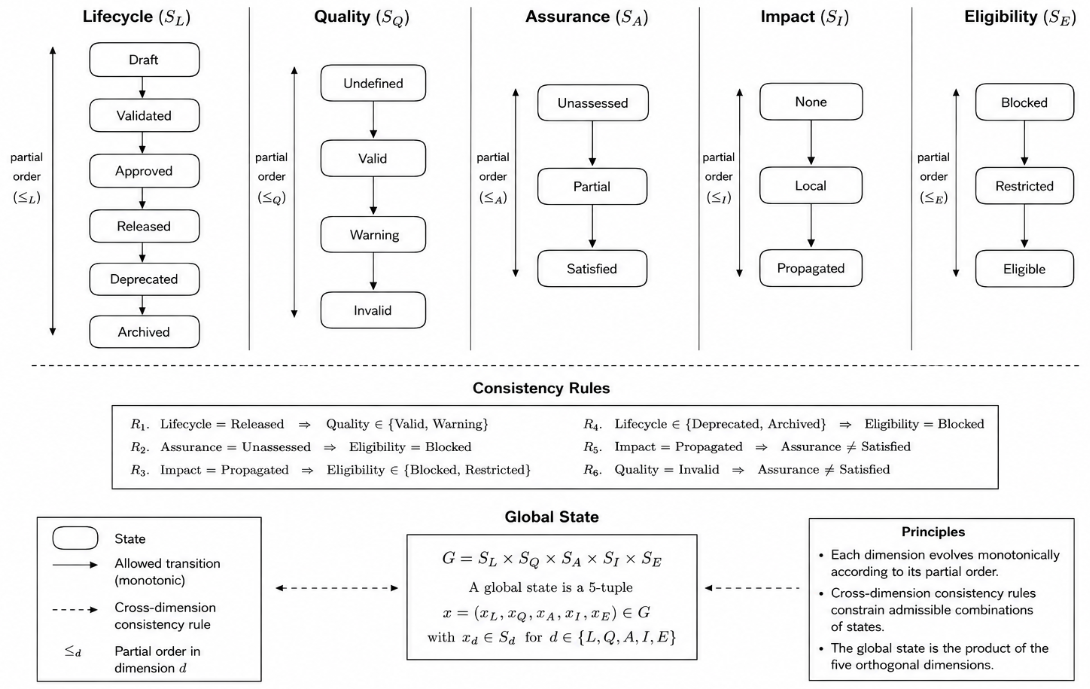
\includegraphics[width=\textwidth]{figures/othogonal_governance_state_machine.png}
	
	\caption{Orthogonal governance state machines composing the ACM governance
		semantics. Lifecycle, quality, impact, and assurance are evaluated as distinct
		state dimensions, while execution eligibility is derived through the evaluation
		function $f(L,Q,A,I)$.}
	\label{fig:governance_state_machine}
\end{figure*}

%%%%%%%%%%%%%%%%%%%%%%%%%%%%%%%%%%%%%%%%%%%%%%%%%%%%%%%%%%%%%%%%%%%%%%%%%%%%%%%%
\subsubsection{Transition Properties}

The governance state machines satisfy the following properties.

\paragraph{Property G1 (Determinism).}

For every governance event, each state machine admits exactly one successor
state.

\paragraph{Property G2 (Orthogonality).}

Each governance dimension evolves independently according to its own transition
function (see Appendix section ~\ref{appendix:governance_orthogonality}).

\paragraph{Property G3 (Composability).}

The global governance state is obtained through the composition of independent
semantic dimensions rather than by constructing a single global automaton.

\paragraph{Property G4 (Extensibility).}

Additional governance dimensions may be introduced without modifying the
existing state machines provided that they expose well-defined evaluation
functions.

These properties considerably simplify future extensions of ACM while
preserving backward compatibility of governance semantics.

The next subsection formalizes how local governance changes propagate through
dependency relationships, enabling global reasoning over complete agentic
configuration graphs.

%%%%%%%%%%%%%%%%%%%%%%%%%%%%%%%%%%%%%%%%%%%%%%%%%%%%%%%%%%%%%%%%%%%%%%%%%%%%%%%%
\subsection{Impact Propagation}
\label{subsec:impact_semantics}

A fundamental objective of ACM is to determine the consequences of a configuration change without modifying the intrinsic properties of unaffected configuration items. Rather than propagating failures indiscriminately through the configuration graph, ACM propagates only governance consequences according to explicitly defined dependency relationships and governance policies.

Impact propagation answers a simple but essential question: \emph{which configuration items may be affected by a change occurring elsewhere in the governed configuration?} The objective is not to predict runtime behavior, but to identify the subset of artifacts whose governance status must be re-evaluated because one or more of their dependencies have changed.

The propagation process is driven by the typed dependency relations defined in the Configuration Graph. Each relationship specifies whether governance effects should be propagated and, if so, under which conditions. Consequently, two dependencies originating from the same configuration item may lead to different propagation behaviors depending on their semantic role and associated governance policy. This policy-driven approach avoids treating all dependencies as equivalent and allows the model to represent heterogeneous governance constraints.

When an ACI revision changes, its direct dependents are examined to determine whether the modification may affect their validity, consistency, or operational readiness. If a dependency is considered governance-relevant, the dependent artifact is marked as impacted. This evaluation is then recursively applied to downstream artifacts until no additional governance states change. The resulting fixed point provides a deterministic and order-independent assessment of the overall impact of the initial modification.

Importantly, impact propagation does not alter the intrinsic lifecycle, quality, or assurance state of dependent artifacts. These properties remain attached to the exact revision to which they belong and therefore preserve their historical meaning. Instead, propagation updates only computed governance states that express the current consequences of the dependency graph. This distinction prevents the loss of provenance and maintains a clear separation between configuration facts and governance interpretations.

The impact computation satisfies the following properties (see Appendix section ~\ref{appendix:impact_propagation}).

\begin{itemize}
	\item \textbf{Determinism.}
	For a given configuration graph and set of governance events, impact computation always produces the same result.
	
	\item \textbf{Monotonicity.}
	Newly detected impacts cannot invalidate previously identified impacted revisions without an explicit recomputation following dependency changes.
	
	\item \textbf{Termination.}
	Since the configuration graph is finite and impact propagates only along declared dependency relations, the propagation algorithm always converges.
	
	\item \textbf{State preservation.}
	Impact is a computed governance property and never modifies the intrinsic lifecycle state of any configuration revision.
\end{itemize}

Figure~\ref{fig:impact_propagation} illustrates the propagation of a local
configuration change through governance dependencies. The directly modified
revision receives the \textit{Local} impact state, while reachable dependent
revisions receive the \textit{Propagated} state. Revisions outside the
resulting impact closure remain in the \textit{None} state.

\begin{figure*}[t]
	\centering
	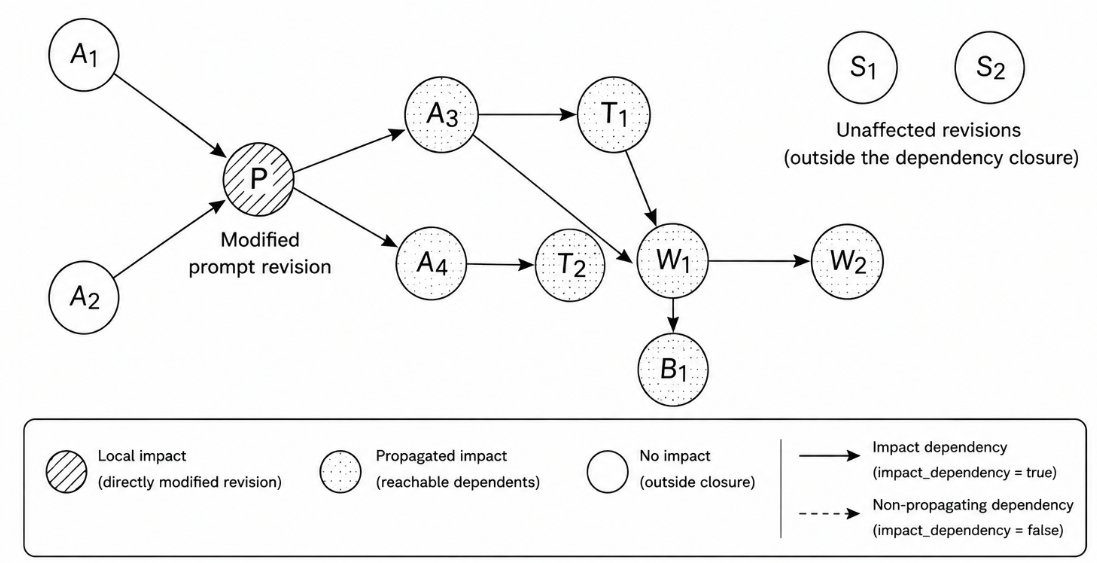
\includegraphics[width=\textwidth]{figures/Impact_propagation_revision.png}
	\caption{
		Impact propagation following the modification of prompt revision $P$.
		The directly modified revision receives a local impact state, while
		reachable dependent revisions receive a propagated impact state.
		Revisions outside the dependency closure remain unaffected.
	}
	\label{fig:impact-propagation}
\end{figure*}

Impact propagation also provides the foundation for subsequent governance analyses. Once impacted artifacts have been identified, additional mechanisms determine whether existing assurance evidence remains applicable, whether execution eligibility must be recomputed, and whether a released baseline can still be considered valid. In this sense, impact propagation acts as the entry point of the governance evaluation pipeline, while assurance and eligibility propagation refine the consequences of the detected changes: the separation between intrinsic lifecycle states and computed impact signals forms the basis for the eligibility and assurance propagation mechanisms introduced in the following sections.



%%%%%%%%%%%%%%%%%%%%%%%%%%%%%%%%%%%%%%%%%%%%%%%%%%%%%%%%%%%%%%%%%%%%%%%%%%%%%%%%
\subsubsection{Propagation Invariants}

Impact propagation satisfies four invariants.

\paragraph{Invariant I1 (Reachability).}

Only reachable nodes may become impacted.

\begin{equation}
I(v)=Propagated
\Longrightarrow
\exists
\pi
:
u
\rightsquigarrow
v.
\label{eq:prop_invariant1}
\end{equation}

\paragraph{Invariant I2 (Termination).}

Since the governance graph is finite, the propagation algorithm always converges.

\paragraph{Invariant I3 (Idempotence).}

Repeated propagation without additional modifications does not alter the final
impact set.

\begin{equation}
P^\ast(P^\ast(X))
=
P^\ast(X).
\label{eq:prop_invariant3}
\end{equation}

\paragraph{Invariant I4 (Monotonicity).}

Introducing additional modified nodes can only increase the propagated impact
set.

\begin{equation}
X
\subseteq
Y
\Longrightarrow
P^\ast(X)
\subseteq
P^\ast(Y).
\label{eq:prop_invariant4}
\end{equation}

%%%%%%%%%%%%%%%%%%%%%%%%%%%%%%%%%%%%%%%%%%%%%%%%%%%%%%%%%%%%%%%%%%%%%%%%%%%%%%%%
\subsubsection{Dependency Categories}

Not every dependency carries identical governance semantics.

ACM distinguishes four conceptual categories.

\begin{enumerate}
    \item Structural dependencies.
    \item Configuration dependencies.
    \item Runtime dependencies.
    \item Assurance dependencies.
\end{enumerate}

Structural dependencies capture graph composition.

Configuration dependencies capture explicit references between immutable
configuration revisions.

Runtime dependencies capture execution-generated relationships.

Assurance dependencies propagate validation requirements introduced by
governance evidence.

Although these dependency categories participate in the same propagation
algorithm, downstream governance policies may assign different consequences to
their respective impacts.

%%%%%%%%%%%%%%%%%%%%%%%%%%%%%%%%%%%%%%%%%%%%%%%%%%%%%%%%%%%%%%%%%%%%%%%%%%%%%%%%
\subsubsection{Complexity}

Assuming an adjacency-list representation, impact propagation is equivalent to
a graph traversal.

Its computational complexity is therefore

\begin{equation}
O(|V|+|E|),
\label{eq:complexity}
\end{equation}

making governance evaluation scalable for large agentic systems.

Since propagation occurs only after governance events rather than continuously,
its computational cost remains proportional to the affected portion of the
configuration graph.

%%%%%%%%%%%%%%%%%%%%%%%%%%%%%%%%%%%%%%%%%%%%%%%%%%%%%%%%%%%%%%%%%%%%%%%%%%%%%%%%
\subsubsection{Illustrative Example}

Assume that a workflow

\[
W
\]

contains an agent

\[
A_1
\]

whose prompt revision is modified.

The prompt immediately becomes

\[
Local.
\]

The associated agent,

workflow,

runtime deployment,

and assurance reports become

\[
Propagated,
\]

because each depends on the modified configuration revision.

Importantly, propagation alone does not imply execution failure.

It merely indicates that governance evaluation should be recomputed before the
corresponding artifacts are considered trustworthy.

%%%%%%%%%%%%%%%%%%%%%%%%%%%%%%%%%%%%%%%%%%%%%%%%%%%%%%%%%%%%%%%%%%%%%%%%%%%%%%%%
\subsubsection{Impact Propagation Summary}

Impact propagation identifies every governance object potentially affected by a
configuration modification while remaining independent from lifecycle,
assurance, and execution authorization.

Its sole responsibility is to maintain the set of revisions whose governance
status requires reevaluation.

The following subsection defines how these governance dimensions are combined
to determine whether an ACI remains authorized for execution.

%%%%%%%%%%%%%%%%%%%%%%%%%%%%%%%%%%%%%%%%%%%%%%%%%%%%%%%%%%%%%%%%%%%%%%%%%%%%%%%%
\subsection{Eligibility Semantics}
\label{subsec:eligibility}

While impact propagation identifies the configuration items potentially affected by a change, eligibility determines whether an ACI revision may still participate in governance operations such as baseline publication, deployment, promotion, or runtime execution. Eligibility therefore represents the operational consequence of the governance evaluation rather than the intrinsic quality of a configuration item.

Unlike lifecycle, quality, or assurance, eligibility is a computed state. It is continuously derived from the current configuration graph, governance policies, dependency states, and applicable evidence. Consequently, the eligibility of a given revision may evolve over time without modifying the revision itself, as changes affecting its dependencies or execution context are reflected through the governance evaluation process.

ACM distinguishes three eligibility states:

\begin{itemize}
	\item \textbf{Eligible}: the revision satisfies all mandatory governance requirements and may participate in the intended governance operation.
	\item \textbf{Restricted}: the revision remains usable but one or more non-blocking conditions require attention before long-term adoption or publication.
	\item \textbf{Blocked}: one or more mandatory governance constraints are violated, preventing the revision from being promoted or used in the considered context.
\end{itemize}

Eligibility is intentionally context-dependent. A revision may be eligible for experimental execution while remaining blocked for release because different governance policies apply to different operational contexts. ACM therefore evaluates eligibility against the applicable governance policy rather than assigning an absolute execution status.

The computation of eligibility follows a conservative strategy. Mandatory violations always take precedence over advisory conditions. A revision becomes \textit{blocked} whenever a mandatory governance requirement cannot be satisfied. Typical blocking conditions include unresolved mandatory references, mandatory dependencies that are no longer acceptable, forbidden runtime overrides, permission escalations, invalid or withdrawn baselines, or any policy violation explicitly designated as blocking.

Less critical situations do not necessarily prevent execution but generate a \textit{restricted}. Examples include impacted dependencies awaiting re-evaluation, optional dependencies with degraded quality, partially completed governance activities, or missing non-mandatory evidence. These situations indicate that the configuration should be reviewed even though it may remain operational under the current governance policy.

Eligibility is propagated through the dependency graph according to the propagation policy associated with each relationship. Blocking conditions affecting a mandatory dependency may therefore prevent downstream artifacts from becoming eligible, whereas optional or non-propagating relationships may have no effect on dependent revisions. This policy-driven propagation prevents local governance issues from unnecessarily affecting unrelated parts of the configuration while ensuring that mandatory constraints remain consistently enforced throughout the governed system.

%%%%%%%%%%%%%%%%%%%%%%%%%%%%%%%%%%%%%%%%%%%%%%%%%%%%%%%%%%%%%%%%%%%%%%%%%%%%%%%%
\subsubsection{Eligibility Function}

Let

\begin{equation}
\mathcal{E}
=
\{
Eligible,
Restricted,
Blocked
\}.
\label{eq:eligibility_state}
\end{equation}

Eligibility is computed by the evaluation function

\begin{equation}
f
:
\mathcal{L}
\times
\mathcal{Q}
\times
\mathcal{A}
\times
\mathcal{I}
\rightarrow
\mathcal{E}.
\label{eq:eligibility_function}
\end{equation}

For every revision

\[
v,
\]

its execution state is therefore

\begin{equation}
E(v)
=
f
(
L(v),
Q(v),
A(v),
I(v)
).
\label{eq:eligibility_execution_state}
\end{equation}

Unlike lifecycle states, eligibility is recomputed whenever one of its input
dimensions evolves. The normative decision constraints follow a set of rules described in Appendix ~\ref{appendix:eligibility_rules}.



%%%%%%%%%%%%%%%%%%%%%%%%%%%%%%%%%%%%%%%%%%%%%%%%%%%%%%%%%%%%%%%%%%%%%%%%%%%%%%%%
\subsubsection{Discussion}

By introducing eligibility as an explicitly computed governance state rather
than embedding authorization decisions within lifecycle transitions, ACM
maintains a strict separation between governance history and operational
authorization.

This distinction is particularly important for long-lived agentic systems,
where execution authorization may change frequently while immutable
configuration revisions remain unchanged.

The following subsection extends this reasoning by introducing assurance
semantics, which formally define how governance evidence contributes to the
global evaluation of configuration trustworthiness.

%%%%%%%%%%%%%%%%%%%%%%%%%%%%%%%%%%%%%%%%%%%%%%%%%%%%%%%%%%%%%%%%%%%%%%%%%%%%%%%%
\subsection{Assurance Semantics}
\label{subsec:assurance_semantics}

Assurance expresses the degree of confidence that can be placed in an ACI revision based on the governance evidence available for that exact revision. Unlike quality, which reflects the outcome of an evaluation, assurance reflects whether the required evaluations have actually been performed and remain applicable. A configuration may therefore have a poor quality assessment while still providing a high level of assurance because all required evaluations were completed and their results are fully traceable. 

Within ACM, assurance therefore answers the following governance question:
\begin{quote}
	\emph{To what extent is the current configuration revision supported by the
		required evidence for its intended governance context?}
\end{quote}

In ACM, assurance is always attached to an immutable revision rather than to a logical configuration item. Every evidence artifact references the exact revision identifier and digest against which it was produced, together with the evaluation scope, execution environment, producer, validity interval, and a snapshot of the dependencies considered during the evaluation. This binding guarantees that governance evidence remains reproducible and cannot be incorrectly reused after a configuration has evolved.

Assurance is evaluated with respect to the governance policy applicable to the considered revision. The policy defines the evidence required before a configuration can be considered sufficiently assessed. Typical evidence may include functional validation, security assessment, compliance verification, performance evaluation, or any other governance activity required by the organization. The corresponding formal definitions of evidence types, applicability rules, dependency snapshots, and composition operators are provided in Appendix~X.

ACM distinguishes three assurance states:

\begin{itemize}
	\item \textbf{Unassessed}: no applicable governance evidence is available for the required evaluations.
	\item \textbf{Partially Assessed}: some required evaluations have been completed, but the available evidence does not yet provide complete coverage.
	\item \textbf{Assessed}: all governance evidence required by the applicable policy is available and remains valid for the evaluated revision.
\end{itemize}

These states describe the completeness of the governance assessment rather than its outcome. Consequently, an ACI revision may simultaneously be \textit{Assessed} and have a quality state indicating that one or more evaluations failed. This distinction is essential because governance requires knowing both whether a configuration has been fully evaluated and what those evaluations concluded.

Assurance evidence remains valid only while the evaluated configuration continues to match the conditions under which the evidence was produced. Any modification affecting the evaluated revision, its dependency snapshot, or other policy-defined evaluation constraints may invalidate previously applicable evidence. Such situations do not alter the historical evidence itself but require the affected configuration to be reassessed before assurance can again be considered complete.

ACM also distinguishes direct and composed assurance. Direct assurance is obtained from evidence explicitly associated with an ACI revision, whereas composed assurance derives from the governance status of dependent artifacts according to the composition policy defined by the governing relationships. By default, assurance is non-transitive: evidence associated with a composite artifact does not automatically validate its constituent artifacts, nor does evidence attached to individual components automatically validate the composite. Composition is performed only when explicitly authorized by the applicable governance policy.

Consequently, ACM distinguishes between:

\begin{itemize}
    \item the \emph{assurance state} intrinsically associated with an ACI
    revision;
    \item the \emph{effective assurance} resulting from dependency propagation
    across the configuration graph.
\end{itemize}

This separation prevents local evidence from being incorrectly interpreted as
evidence for an entire composite configuration (see Appendix ~\ref{appendix:assurance_semantics} for the detailed formalism)

%%%%%%%%%%%%%%%%%%%%%%%%%%%%%%%%%%%%%%%%%%%%%%%%%%%%%%%%%%%%%%%%%%%%%%%%%%%%%%%%
\subsubsection{Assurance State Space}

Let

\begin{equation}
\mathcal{A}
=
\{
\texttt{unassessed},
\texttt{partially\_assessed},
\texttt{assessed}
\}
\label{eq:assurance_states}
\end{equation}

denote the assurance state space.

Each ACI revision is associated with an assurance mapping

\begin{equation}
A_n :
V
\rightarrow
\mathcal{A},
\label{eq:assurance_mapping}
\end{equation}

where the notation \(A_n\) is intentionally used to distinguish
\emph{Assurance} from the quality notation introduced previously.

The three assurance states have the following semantics.

\begin{itemize}
    \item \textbf{\texttt{unassessed}}: no applicable evidence exists for the
    considered revision.

    \item \textbf{\texttt{partially\_assessed}}: only a subset of the required
    evidence is currently available or applicable.

    \item \textbf{\texttt{assessed}}: all required evidence applicable to the
    considered governance context is available and valid.
\end{itemize}

Importantly, the state
\texttt{assessed}
does \emph{not} imply that evaluations were successful.
It only indicates that the required evaluation process has been completed.

Thus,

\[
A_n(v)=\texttt{assessed}
\]

is compatible with

\[
Q(v)=\texttt{nok},
\]

which corresponds to a completely evaluated component that failed one or more
mandatory evaluation criteria.


%%%%%%%%%%%%%%%%%%%%%%%%%%%%%%%%%%%%%%%%%%%%%%%%%%%%%%%%%%%%%%%%%%%%%%%%%%%%%%%%
\subsubsection{Applicable Evidence}

Not every recorded evaluation remains applicable indefinitely.

An evidence item may become obsolete because one of the artifacts on which it
depends has evolved, because the execution environment has changed, or because
its declared validity period has expired.

Accordingly, ACM introduces the notion of
\emph{applicable evidence}.

An evidence item
\(e\)
is applicable to revision
\(v\)
iff all of the following conditions hold:

\begin{enumerate}
    \item the targeted revision identifier matches;
    \item the recorded digest matches the current revision;
    \item the evaluation scope includes the considered revision;
    \item the execution environment satisfies the declared constraints;
    \item the evidence has not expired;
    \item every referenced dependency remains unchanged.
\end{enumerate}

Formally,

\begin{equation}
Applicable(e,v)
=
\bigwedge_{i=1}^{6}
C_i(e,v),
\label{eq:applicable_evidence}
\end{equation}

where each predicate
\(C_i\)
corresponds to one of the applicability conditions listed above.

%%%%%%%%%%%%%%%%%%%%%%%%%%%%%%%%%%%%%%%%%%%%%%%%%%%%%%%%%%%%%%%%%%%%%%%%%%%%%%%%
\subsubsection{Discussion}

The proposed assurance semantics intentionally separates evidence completeness
from evaluation outcomes. This distinction enables ACM to reason independently
about governance confidence and operational quality, avoiding ambiguities that
frequently arise when these concepts are merged into a single status.

Moreover, because assurance is attached to immutable revisions and propagated
deterministically through the configuration graph, every assurance decision
remains fully traceable, reproducible and independently auditable. The next
subsection builds upon these semantics to define how governance states
propagate through dependency relationships across the complete configuration
graph.

%%%%%%%%%%%%%%%%%%%%%%%%%%%%%%%%%%%%%%%%%%%%%%%%%%%%%%%%%%%%%%%%%%%%%%%%%%%%%%%%
\subsection{Governance State Propagation}
\label{subsec:governance_state_propagation}

The previous subsections introduced the semantics of the individual governance
dimensions governing each Agentic Configuration Item (ACI). In practice,
however, governance decisions rarely concern isolated artifacts. Agentic
systems are composed of interconnected prompts, agents, workflows, policies,
tools and models whose governance properties are interdependent. Consequently,
a modification affecting one configuration item may require the re-evaluation
of several dependent artifacts.

A central contribution of ACM is therefore the introduction of a formal
governance propagation model. Rather than propagating lifecycle, quality or
assurance states directly, ACM propagates the consequences of governance
changes according to the semantics of each state dimension. This distinction,
which emerged from the audit of the reference model, avoids the incorrect
assumption that the governance state of a composite artifact should simply
mirror the state of one of its dependencies.

For example, the deprecation of a prompt does not automatically imply that the
agent using it also becomes deprecated. Instead, the agent becomes impacted,
its assurance may become partially assessed, and its eligibility for inclusion
in a future release baseline may be downgraded. The intrinsic lifecycle of the
agent remains unchanged until an explicit governance decision is taken.

Figure~\ref{fig:agent_state_before_after} illustrates the non-destructive
propagation of governance state for a single agent. A change to a required
prompt revision does not modify the agent revision or its intrinsic lifecycle
and quality states. Instead, the propagation process recalculates the agent's
impact, assurance, and eligibility states from the updated dependency context.
\begin{figure*}[t]
	\centering
	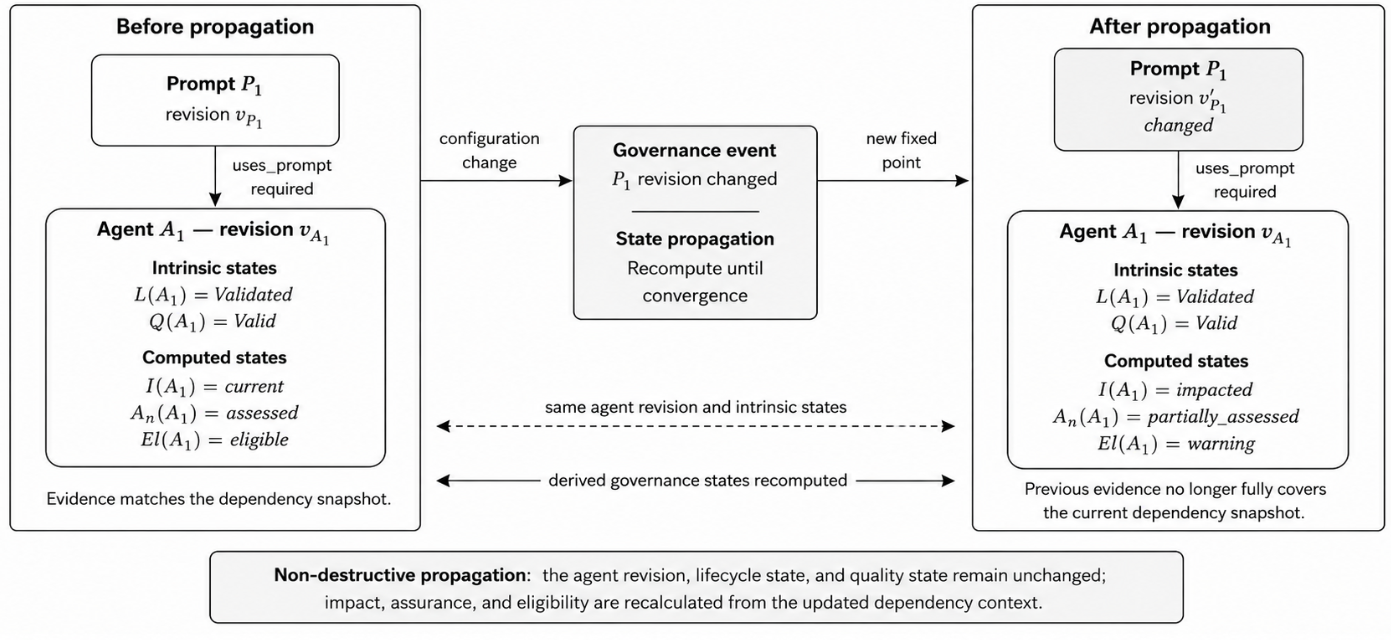
\includegraphics[width=\textwidth]{figures/non_destructive_state_propagation.png}
	
	\caption{Non-destructive governance state propagation for an agent. A change
		to a required prompt revision preserves the agent revision and its intrinsic
		lifecycle and quality states, while the derived impact, assurance, and
		eligibility states are recomputed from the updated dependency context.}
	\label{fig:agent_state_before_after}
\end{figure*}

%%%%%%%%%%%%%%%%%%%%%%%%%%%%%%%%%%%%%%%%%%%%%%%%%%%%%%%%%%%%%%%%%%%%%%%%%%%%%%%%
\subsubsection{Configuration Graph}

Governance propagation is evaluated over the configuration graph introduced in
Section~\ref{sec:reference_model}.

Let

\begin{equation}
G_c=(V_c,E_c)
\label{eq:configuration_graph}
\end{equation}

denote the directed configuration graph, where

\begin{itemize}
    \item $V_c$ is the set of ACI revisions,
    \item $E_c$ is the set of governance relationships.
\end{itemize}

Unlike previous sections, the notation $G_c$ explicitly refers to the
\textbf{Configuration Graph}. This notation is used consistently throughout the
remainder of the manuscript and must not be confused with the Runtime Graph
introduced later.

Each edge

\[
e=(u,v)\in E_c
\]

represents a dependency from revision $u$ towards revision $v$.

Every relationship carries governance metadata describing how propagation shall
be performed.

%%%%%%%%%%%%%%%%%%%%%%%%%%%%%%%%%%%%%%%%%%%%%%%%%%%%%%%%%%%%%%%%%%%%%%%%%%%%%%%%
\subsubsection{Relationship Semantics}

Governance propagation depends on the semantics of the relationship connecting
two artifacts.

Each relationship is characterized by four governance attributes:

\begin{itemize}
    \item whether the dependency is mandatory;
    \item the propagation policy;
    \item whether assurance depends on this relationship;
    \item whether impact propagates through this relationship.
\end{itemize}

Formally, every edge

\[
e\in E_c
\]

is associated with

\begin{equation}
\Pi(e)=
(
required,
policy,
impact,
assurance
)
\label{eq:relationship_policy}
\end{equation}

where

\begin{itemize}
    \item $required\in\{true,false\}$,
    \item $policy\in
    \{
    blocking,
    warning,
    informational,
    none
    \}$,
    \item $impact\in\{true,false\}$,
    \item $assurance\in\{true,false\}$.
\end{itemize}

These attributes determine which governance dimensions may propagate through
the relationship (see section ~\ref{appendix:state_propagation} in Appendix for the propagation principles)

%%%%%%%%%%%%%%%%%%%%%%%%%%%%%%%%%%%%%%%%%%%%%%%%%%%%%%%%%%%%%%%%%%%%%%%%%%%%%%%%
\subsubsection{Propagation Algorithm}

Governance propagation proceeds according to the following sequence.

\begin{enumerate}
    \item Detect local governance changes.
    \item Compute impacted dependencies.
    \item Re-evaluate evidence applicability.
    \item Recompute effective assurance.
    \item Recompute effective quality.
    \item Re-evaluate eligibility.
    \item Iterate until a fixed point is reached.
\end{enumerate}

For an acyclic configuration graph, the computation requires

\begin{equation}
\mathcal{O}
\left(
|V_c|+|E_c|
\right)
\label{eq:propagation_complexity}
\end{equation}

whereas cyclic dependency structures require an iterative fixed-point
computation over the strongly connected components.

\subsubsection{Fixed-Point Semantics of Governance Propagation}
\label{subsec:fixed_point_semantics}

The propagation semantics introduced in the previous sections have been defined
through local governance rules associated with dependency relationships. This
operational description can be formalized more rigorously by viewing governance
propagation as the computation of the least fixed point of a monotone operator
over a finite lattice. This formulation establishes the formal semantics of
governance propagation independently of any implementation strategy and
provides a formal justification for its termination, determinism, and
implementation independence.

The governance evaluation intentionally distinguishes between
\emph{intrinsic} properties, which are permanently associated with immutable
ACI revisions, and \emph{derived} properties, which are automatically
recomputed according to dependency relationships and governance policies.

For every ACI revision $v$, let

\[
D(v)=
\left(
L(v),
Q_d(v),
A_d(v)
\right)
\]

denote the intrinsic governance descriptor, where $L$ is the lifecycle state,
$Q_d$ the declared quality state, and $A_d$ the direct assurance state
determined from the evidence attached to the revision.

Propagation computes the derived governance descriptor

\[
X(v)=
\left(
I(v),
Q(v),
A(v),
E(v)
\right),
\]

where $I$, $Q$, $A$, and $E$ respectively denote the impact, effective quality,
effective assurance, and execution eligibility associated with the revision.

Unlike lifecycle states, these dimensions evolve automatically according to
dependency relationships and therefore constitute the state space over which
governance propagation operates.

%%%%%%%%%%%%%%%%%%%%%%%%%%%%%%%%%%%%%%%%%%%%%%%%%%%%%%%%%%%%%%%%%%%%%%%%%%%%%%%

\paragraph{Governance State Lattice}

Each propagated governance dimension is partially ordered from the least
restrictive state to the most restrictive one.

For impact propagation,

\[
Current
\;\sqsubseteq\;
Impacted
\;\sqsubseteq\;
Stale.
\]

For effective quality,

\[
OK
\;\sqsubseteq\;
Unknown
\;\sqsubseteq\;
ToImprove
\;\sqsubseteq\;
NOK.
\]

For effective assurance,

\[
Assessed
\;\sqsubseteq\;
PartiallyAssessed
\;\sqsubseteq\;
Unassessed.
\]

Finally, execution eligibility satisfies

\[
Eligible
\;\sqsubseteq\;
Restricted
\;\sqsubseteq\;
Blocked.
\]

Each governance dimension forms a finite chain and therefore a finite lattice.

The governance state associated with one revision belongs to the product lattice

\[
\mathcal{S}
=
\mathcal{I}
\times
\mathcal{Q}
\times
\mathcal{A}
\times
\mathcal{E},
\]

ordered component-wise.

Given a finite configuration graph

\[
G_c=(V_c,E_c),
\]

the complete governance state of the configuration is represented by the
mapping

\[
X:V_c\rightarrow\mathcal{S},
\]

whose domain

\[
\mathcal{L}
=
\mathcal{S}^{V_c}
\]

is itself a finite lattice.

%%%%%%%%%%%%%%%%%%%%%%%%%%%%%%%%%%%%%%%%%%%%%%%%%%%%%%%%%%%%%%%%%%%%%%%%%%%%%%%

\paragraph{Relationship Transfer Functions}

Each dependency relationship contributes to governance propagation through a
local transfer function.

For every dependency

\[
e=(u,v)\in E_c,
\]

let

\[
\tau_e:
\mathcal{S}
\rightarrow
\mathcal{S}
\]

denote the transfer function associated with the governance semantics of that
relationship.

Its behavior depends on the relationship attributes defined by the reference
model (required dependencies, assurance propagation, impact propagation,
blocking policies, and other governance constraints), but it satisfies the
following monotonicity property:

\[
x
\sqsubseteq
y
\Longrightarrow
\tau_e(x)
\sqsubseteq
\tau_e(y).
\]

Intuitively, a more degraded dependency can never produce a less restrictive
governance state.

%%%%%%%%%%%%%%%%%%%%%%%%%%%%%%%%%%%%%%%%%%%%%%%%%%%%%%%%%%%%%%%%%%%%%%%%%%%%%%%

\paragraph{Global Propagation Operator}

Let

\[
Pred(v)
=
\left\{
u\in V_c
\mid
(u,v)\in E_c
\right\}
\]

denote the predecessors of revision $v$.

The propagation semantics are defined by the global operator

\[
F:
\mathcal{L}
\rightarrow
\mathcal{L},
\]

such that

\[
F(X)(v)
=
X(v)
\sqcup
B(v)
\sqcup
\bigvee_{u\in Pred(v)}
\tau_{(u,v)}
\!\left(
X(u)
\right),
\]

where $B(v)$ denotes the local governance state directly inferred from the
revision itself, independently of propagated dependencies, and $\sqcup$
represents the lattice join.

The propagation operator is inflationary,

\[
X
\sqsubseteq
F(X),
\]

and monotone,

\[
X
\sqsubseteq
Y
\Longrightarrow
F(X)
\sqsubseteq
F(Y).
\]

Consequently, each propagation step preserves or strengthens governance
constraints while preventing inconsistent state regressions.

%%%%%%%%%%%%%%%%%%%%%%%%%%%%%%%%%%%%%%%%%%%%%%%%%%%%%%%%%%%%%%%%%%%%%%%%%%%%%%%

\paragraph{Least Fixed-Point Semantics}

Propagation starts from the least governance state,

\[
X_0=\bot,
\]

and repeatedly applies the propagation operator,

\[
X_{k+1}
=
F(X_k).
\]

Since $\mathcal{L}$ is a finite lattice and $F$ is monotone, the sequence

\[
X_0
\sqsubseteq
X_1
\sqsubseteq
X_2
\sqsubseteq
\cdots
\]

is monotonically increasing and necessarily stabilizes after a finite number
of iterations.

The resulting governance state is therefore defined as

\[
X^\ast
=
\operatorname{lfp}(F),
\]

that means that the stabilized valuation $\iota^{*}$ is the least fixed point of
$\widehat{\mathrm{Prop}}$ above the initial impact valuation
$\iota^{(0)}$. It therefore represents the minimal stable impact assignment
that preserves the revisions directly affected by the triggering governance
event.

%%%%%%%%%%%%%%%%%%%%%%%%%%%%%%%%%%%%%%%%%%%%%%%%%%%%%%%%%%%%%%%%%%%%%%%%%%%%%%%

\paragraph{Property 1 (Termination)}

For every finite ACM configuration graph, iterative governance propagation
terminates after a finite number of state updates.

\emph{Rationale.}
The global governance domain $\mathcal{L}$ is a finite lattice.
Since $F$ is inflationary, every iteration produces an increasing chain.
Every increasing chain in a finite lattice is finite; therefore the iterative
evaluation necessarily reaches a stable governance state.

%%%%%%%%%%%%%%%%%%%%%%%%%%%%%%%%%%%%%%%%%%%%%%%%%%%%%%%%%%%%%%%%%%%%%%%%%%%%%%%

\paragraph{Property 2 (Existence of a Least Fixed Point)}

The ACM propagation operator always admits a unique least fixed point.

\emph{Rationale.}
Because $\mathcal{L}$ is a complete finite lattice and $F$ is monotone, the
Knaster--Tarski fixed-point theorem guarantees the existence of a least fixed
point. Iterative application of $F$ from the bottom element computes exactly
this least fixed point.

%%%%%%%%%%%%%%%%%%%%%%%%%%%%%%%%%%%%%%%%%%%%%%%%%%%%%%%%%%%%%%%%%%%%%%%%%%%%%%%

\paragraph{Property 3 (Deterministic Governance Evaluation)}

The governance state computed by ACM is uniquely determined by the
configuration graph, the intrinsic revision states, and the relationship
policies, independently of the order in which propagation rules are evaluated.

\emph{Rationale.}
Every fair propagation strategy computes the same least fixed point of the
monotone operator $F$. Consequently, recursive graph traversals, work-list
algorithms, or incremental propagation strategies all converge toward the same
governance state.

%%%%%%%%%%%%%%%%%%%%%%%%%%%%%%%%%%%%%%%%%%%%%%%%%%%%%%%%%%%%%%%%%%%%%%%%%%%%%%%

This fixed-point formulation establishes the formal semantics of governance
propagation independently of any particular implementation. Whether ACM is
implemented through recursive graph traversal, work-list evaluation, or
incremental update algorithms, every compliant implementation is required to
compute the same least fixed point, thereby guaranteeing deterministic,
reproducible, and implementation-independent governance evaluation.
%%%%%%%%%%%%%%%%%%%%%%%%%%%%%%%%%%%%%%%%%%%%%%%%%%%%%%%%%%%%%%%%%%%%%%%%%%%%%%%%
\subsubsection{Illustrative Example}

Figure~\ref{fig:governance_propagation} illustrates the propagation of a prompt
deprecation through an agentic configuration. The prompt revision becomes
\texttt{deprecated}; the dependent agent becomes \texttt{impacted}; its
effective assurance is downgraded to
\texttt{partially\_assessed}; and its eligibility changes from
\texttt{eligible} to
\texttt{warning}. Importantly, neither the lifecycle nor the declared quality
of the agent is modified. This example illustrates the central principle of ACM
that governance propagation affects derived governance states rather than
intrinsic configuration properties.

%%%%%%%%%%%%%%%%%%%%%%%%%%%%%%%%%%%%%%%%%%%%%%%%%%%%%%%%%%%%%%%%%%%%%%%%%%%%%%%%
% Figure to be inserted here
%
% Figure:
% Governance State Propagation
%
% (TikZ IEEE academic style)
%
%%%%%%%%%%%%%%%%%%%%%%%%%%%%%%%%%%%%%%%%%%%%%%%%%%%%%%%%%%%%%%%%%%%%%%%%%%%%%%%%
% Figure: Governance State Propagation
%%%%%%%%%%%%%%%%%%%%%%%%%%%%%%%%%%%%%%%%%%%%%%%%%%%%%%%%%%%%%%%%%%%%%%%%%%%%%%%%
\begin{figure}[t]
\centering
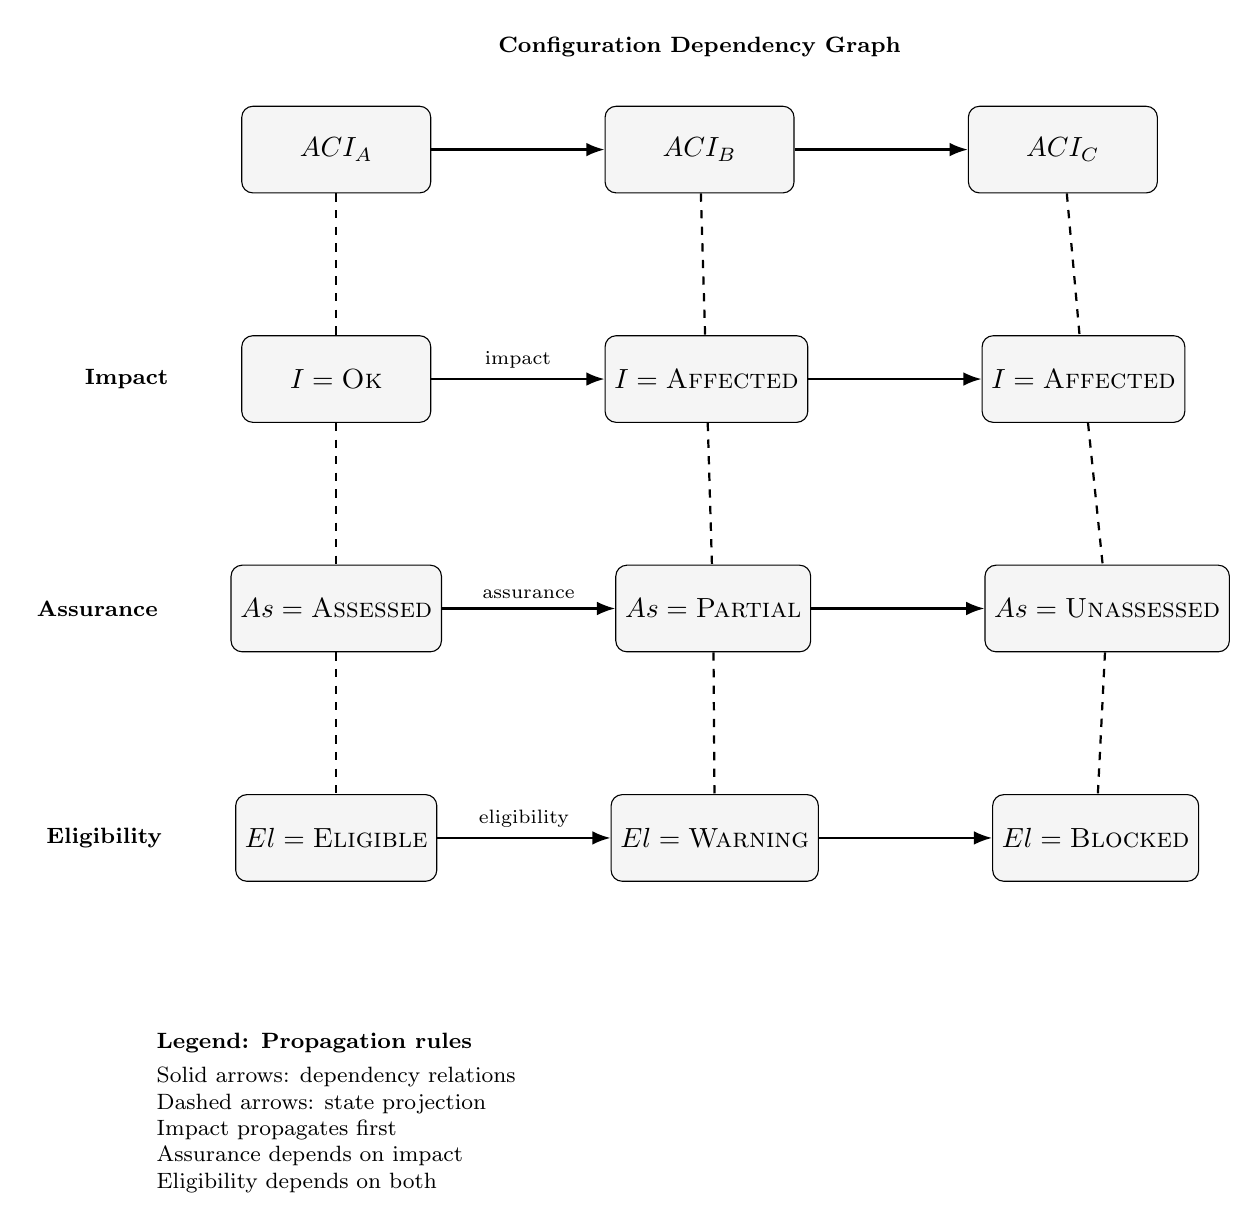
\begin{tikzpicture}[
    >=Latex,
    node distance=18mm and 22mm,
    aci/.style={
        draw,
        rounded corners,
        minimum width=24mm,
        minimum height=11mm,
        align=center,
        fill=gray!8
    },
    flow/.style={
        ->,
        thick
    },
    prop/.style={
        dashed,
        thick
    },
    annot/.style={
        font=\footnotesize,
        align=center
    }
]

%-------------------------------------------------
% Configuration graph
%-------------------------------------------------

\node[aci] (A) {$ACI_A$};
\node[aci,right=of A] (B) {$ACI_B$};
\node[aci,right=of B] (C) {$ACI_C$};

\draw[flow] (A)--(B);
\draw[flow] (B)--(C);

\node[annot,above=5mm of B]
{\textbf{Configuration Dependency Graph}};

%-------------------------------------------------
% Impact propagation
%-------------------------------------------------

\node[aci,below=18mm of A] (IA) {$I=\textsc{Ok}$};
\node[aci,right=of IA] (IB) {$I=\textsc{Affected}$};
\node[aci,right=of IB] (IC) {$I=\textsc{Affected}$};

\draw[prop] (A)--(IA);
\draw[prop] (B)--(IB);
\draw[prop] (C)--(IC);

\draw[flow] (IA)--node[above,font=\scriptsize]{impact}(IB);
\draw[flow] (IB)--node[above,font=\scriptsize]{}(IC);

\node[annot,left=8mm of IA]
{\textbf{Impact}};

%-------------------------------------------------
% Assurance propagation
%-------------------------------------------------

\node[aci,below=18mm of IA] (AA) {$As=\textsc{Assessed}$};
\node[aci,right=of AA] (AB) {$As=\textsc{Partial}$};
\node[aci,right=of AB] (AC) {$As=\textsc{Unassessed}$};

\draw[prop] (IA)--(AA);
\draw[prop] (IB)--(AB);
\draw[prop] (IC)--(AC);

\draw[flow] (AA)--node[above,font=\scriptsize]{assurance}(AB);
\draw[flow] (AB)--(AC);

\node[annot,left=8mm of AA]
{\textbf{Assurance}};

%-------------------------------------------------
% Eligibility propagation
%-------------------------------------------------

\node[aci,below=18mm of AA] (EA) {$El=\textsc{Eligible}$};
\node[aci,right=of EA] (EB) {$El=\textsc{Warning}$};
\node[aci,right=of EB] (EC) {$El=\textsc{Blocked}$};

\draw[prop] (AA)--(EA);
\draw[prop] (AB)--(EB);
\draw[prop] (AC)--(EC);

\draw[flow] (EA)--node[above,font=\scriptsize]{eligibility}(EB);
\draw[flow] (EB)--(EC);

\node[annot,left=8mm of EA]
{\textbf{Eligibility}};

%-------------------------------------------------
% Legend
%-------------------------------------------------

\node[
align=left,
below=18mm of EA,
font=\footnotesize
]
{
\textbf{Legend: Propagation rules}\\[1mm]
Solid arrows: dependency relations\\
Dashed arrows: state projection\\
Impact propagates first\\
Assurance depends on impact\\
Eligibility depends on both
};

\end{tikzpicture}

\caption{Governance state propagation across the configuration graph.
A structural dependency first propagates impact, which subsequently influences
assurance evaluation and finally execution eligibility. The three governance
dimensions remain conceptually independent while being evaluated in a
deterministic order.}
\label{fig:governance_propagation}
\end{figure}
%%%%%%%%%%%%%%%%%%%%%%%%%%%%%%%%%%%%%%%%%%%%%%%%%%%%%%%%%%%%%%%%%%%%%%%%%%%%%%%%

%%%%%%%%%%%%%%%%%%%%%%%%%%%%%%%%%%%%%%%%%%%%%%%%%%%%%%%%%%%%%%%%%%%%%%%%%%%%%%%%
\subsection{Runtime Semantics}
\label{subsec:runtime_semantics}

The governance semantics defined so far describe how configuration states evolve
within the immutable configuration graph. Runtime execution introduces an
additional dimension that cannot be represented solely by static configuration
artifacts. Agent executions create transient observations whose purpose is not
to modify the governed configuration but to record how a released baseline is
instantiated during execution.

Accordingly, ACM distinguishes the \emph{Configuration Graph}, which contains
immutable governed revisions, from the \emph{Runtime Graph}, which represents
the execution state derived from a specific released baseline. Runtime
observations never alter immutable configuration revisions. Instead, they are
associated with the corresponding governed artifacts through stable revision
identifiers and provenance relationships.

The Runtime Graph is constructed from an ordered sequence of normalized runtime
events. Each event captures an observable execution transition together with the
identifier of the corresponding governed revision. Because runtime observations
are represented independently from framework-specific execution traces, the same
governance semantics can be applied to heterogeneous execution frameworks after
semantic projection into the ACM reference model.

Rather than storing successive runtime snapshots, ACM defines the runtime state
as the result of replaying the normalized event sequence from a released
baseline. Starting from the immutable configuration represented by the baseline,
runtime events are deterministically applied in chronological order to
reconstruct the Runtime Graph corresponding to any observation point.

This separation provides two complementary benefits. First, released
configurations remain immutable throughout execution, preserving configuration
integrity and provenance. Second, runtime reconstruction becomes independent of
the execution framework, provided that equivalent normalized events are
available. Consequently, runtime analyses, governance verification, and
conformance checking operate on a canonical Runtime Graph rather than on
framework-specific execution representations.

The replay semantics are intentionally defined independently of the propagation
operator introduced in Section~\ref{sec:propagation_semantics}. Propagation
computes the stabilized governance state associated with immutable
configurations, whereas replay reconstructs the execution state generated from a
released baseline. These two mechanisms therefore address complementary
concerns: governance evaluation determines the valid configuration to be
executed, while runtime replay reconstructs how that configuration was actually
executed.

The formal definition of normalized runtime events, the replay function, the
incremental reconstruction procedure, and the associated correctness properties
are presented in Appendix~A.7. ~\ref{appendix:runtime_semantics}.

\subsection{Formal Properties}
\label{sec:formal_properties}

The governance semantics defined in the previous subsections satisfy a number of
formal properties that ensure the consistency, reproducibility, and
predictability of ACM evaluations. These properties follow directly from the
state spaces, evaluation functions, propagation semantics, and runtime replay
model introduced throughout Section~5.

First, the impact propagation semantics are monotone over the finite impact
lattice defined in Appendix~A.3. Consequently, iterative propagation converges
toward the least fixed point above the initial impact valuation, while the
reference worklist algorithm computes the same stabilized result under any fair
evaluation strategy. The corresponding proofs are provided in
Appendix~A.6.

Second, runtime replay is deterministic. Given an immutable released baseline
and an identical ordered sequence of normalized runtime events, replay always
reconstructs the same Runtime Graph. This property guarantees that runtime
observations remain reproducible independently of the underlying execution
framework after semantic projection into the ACM reference model. The formal
replay model and proof of determinism are presented in Appendix~A.7.

Together, these properties establish that governance evaluation and runtime
reconstruction are reproducible and implementation-independent. For identical
governed configurations and equivalent normalized runtime observations, ACM
always produces identical governance states and identical reconstructed Runtime
Graphs. This determinism provides the foundation for reproducible governance
verification, impact analysis, runtime conformance checking, and assurance
evaluation across heterogeneous agentic frameworks.

The complete proofs, together with the complexity analysis and additional formal
results, are presented in Appendix~A.8.


























\section{Operationalization}
\label{sec:operationalization}

The purpose of this section is not to define another execution framework but to demonstrate that the proposed reference model is operationalizable without introducing framework-specific concepts into its governance semantics. The operationalization deliberately separates governance semantics from implementation details. The ACM metamodel, lifecycle semantics, and validation rules are independent of programming language, persistence technology, communication protocol, or execution framework. The Python implementation therefore serves only as one concrete realization of the reference model, demonstrating implementability rather than prescribing a specific software architecture. The experimental methodology is depicted in Figure ~\ref{fig:experimental_protocol}.

\begin{figure*}[t]
	\centering
	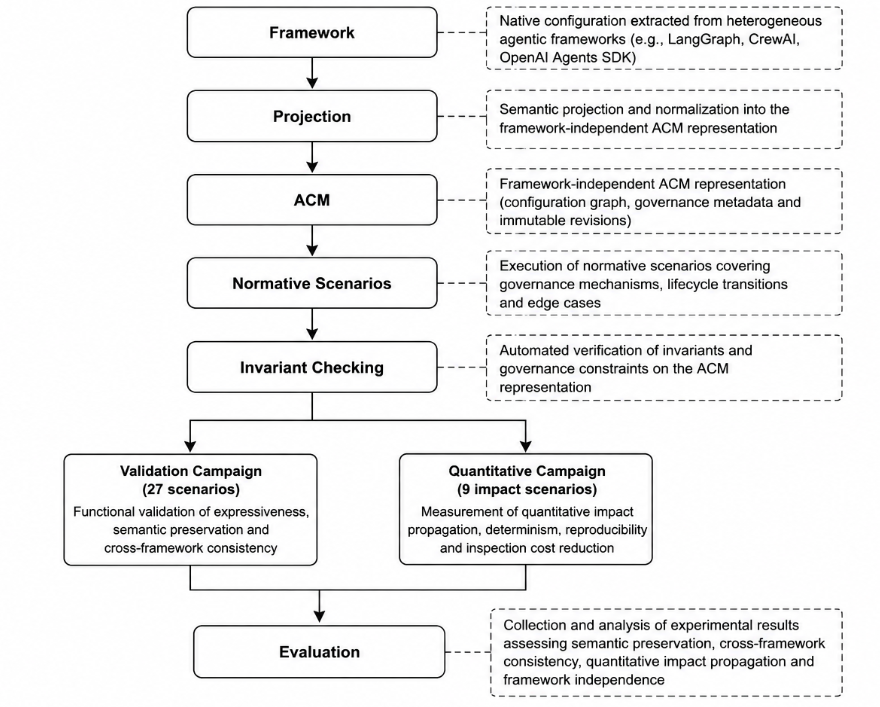
\includegraphics[width=0.5\textwidth]{figures/experimental_protocol.png}
	\caption{Overview of the experimental methodology. Native framework configurations are projected into the ACM reference model through semantic projection, validated using normative governance scenarios and automated invariant checking, and finally evaluated with respect to model expressiveness, semantic preservation, and framework independence.}
	\label{fig:experimental_protocol}
\end{figure*}

\subsection{Reference Architecture}
\label{subsec:reference_architecture}

The ACM reference model is intentionally independent of any particular agentic framework. Its operationalization therefore adopts a layered architecture that cleanly separates framework-specific extraction from framework-independent governance. This separation preserves the conceptual independence of the reference model while allowing heterogeneous agentic systems to be represented through a common governed configuration.

Figure~\ref{fig:acm_reference_architecture} presents the reference architecture adopted by the prototype implementation. Native framework artifacts are first extracted by framework-specific projection adapters before being transformed into canonical ACM representations. All subsequent governance operations are then performed exclusively on normalized ACM objects, independently of the originating framework.


%%%%%%%%%%%%%%%%%%%%%%%%%%%%%%%%%%%%%%%%%%%%%%%%%%%%%%%%%%%%%%%%%%%%%%%%%%%%%%%%
% Required packages and libraries
%
% \usepackage{tikz}
% \usetikzlibrary{
%     arrows.meta,
%     positioning,
%     fit,
%     backgrounds,
%     calc
% }
%%%%%%%%%%%%%%%%%%%%%%%%%%%%%%%%%%%%%%%%%%%%%%%%%%%%%%%%%%%%%%%%%%%%%%%%%%%%%%%%

\begin{figure}[t]
\centering

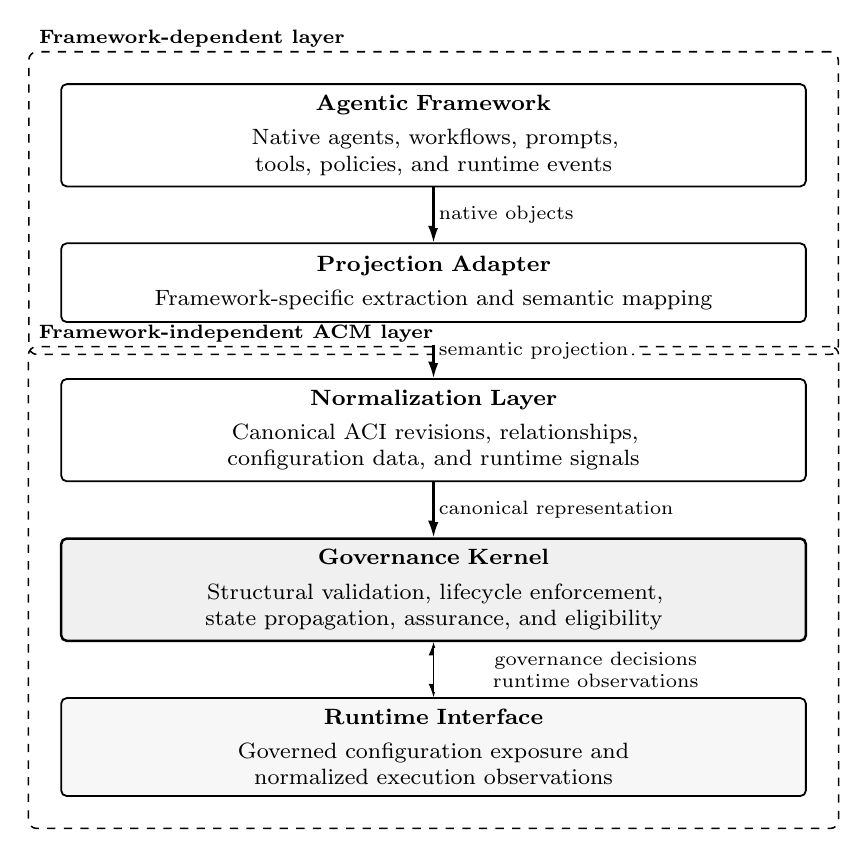
\begin{tikzpicture}[
    font=\footnotesize,
    >=Latex,
    node distance=7mm,
    stage/.style={
        draw,
        rounded corners=2pt,
        minimum width=0.78\columnwidth,
        minimum height=10mm,
        text width=0.68\columnwidth,
        align=center,
        line width=0.65pt,
        fill=white,
        inner sep=4pt
    },
    kernel/.style={
        stage,
        line width=0.9pt,
        fill=gray!12
    },
    runtime/.style={
        stage,
        fill=gray!6
    },
    flow/.style={
        -{Latex[length=2.1mm,width=1.4mm]},
        line width=0.8pt
    },
    bidirectional/.style={
        {Latex[length=2mm,width=1.3mm]}-
        {Latex[length=2mm,width=1.3mm]},
        line width=0.8pt
    },
    edgeLabel/.style={
        font=\scriptsize,
        fill=white,
        inner sep=1.5pt,
        align=center
    },
    boundary/.style={
        draw,
        dashed,
        rounded corners=3pt,
        line width=0.55pt,
        inner sep=4mm
    },
    boundaryLabel/.style={
        font=\scriptsize\bfseries,
        fill=white,
        inner sep=1pt
    }
]

%------------------------------------------------------------------------------
% Main processing pipeline
%------------------------------------------------------------------------------

\node[stage] (framework) {
    \textbf{Agentic Framework}\\[1mm]
    Native agents, workflows, prompts, tools,
    policies, and runtime events
};

\node[stage, below=of framework] (adapter) {
    \textbf{Projection Adapter}\\[1mm]
    Framework-specific extraction and semantic mapping
};

\node[stage, below=of adapter] (normalization) {
    \textbf{Normalization Layer}\\[1mm]
    Canonical ACI revisions, relationships,
    configuration data, and runtime signals
};

\node[kernel, below=of normalization] (governance) {
    \textbf{Governance Kernel}\\[1mm]
    Structural validation, lifecycle enforcement,
    state propagation, assurance, and eligibility
};

\node[runtime, below=of governance] (runtime) {
    \textbf{Runtime Interface}\\[1mm]
    Governed configuration exposure and
    normalized execution observations
};

%------------------------------------------------------------------------------
% Directed processing flow
%------------------------------------------------------------------------------

\draw[flow]
    (framework.south)
    --
    node[edgeLabel, right]
    {native objects}
    (adapter.north);

\draw[flow]
    (adapter.south)
    --
    node[edgeLabel, right]
    {semantic projection}
    (normalization.north);

\draw[flow]
    (normalization.south)
    --
    node[edgeLabel, right]
    {canonical representation}
    (governance.north);

%------------------------------------------------------------------------------
% Bidirectional runtime interaction
%------------------------------------------------------------------------------

\draw[<->]
    (governance.south)
    --
    node[edgeLabel, right, text width=40mm]
    {governance decisions\\
     runtime observations}
    (runtime.north);

%------------------------------------------------------------------------------
% Responsibility boundaries
% These elements are placed behind the main nodes.
%------------------------------------------------------------------------------

\begin{scope}[on background layer]

    \node[
        boundary,
        fit=(framework)(adapter)
    ] (frameworkBoundary) {};

    \node[
        boundary,
        fit=(normalization)(governance)(runtime)
    ] (acmBoundary) {};

\end{scope}

%------------------------------------------------------------------------------
% Boundary labels
%------------------------------------------------------------------------------

\node[
    boundaryLabel,
    anchor=south west
] at ($(frameworkBoundary.north west)+(1mm,0)$)
{
    Framework-dependent layer
};

\node[
    boundaryLabel,
    anchor=south west
] at ($(acmBoundary.north west)+(1mm,0)$)
{
    Framework-independent ACM layer
};

\end{tikzpicture}

\caption{Reference architecture for the operationalization of ACM. Native
framework constructs are extracted through framework-specific projection
adapters and translated into canonical representations before entering the
framework-independent governance kernel. The runtime interface exposes
governance decisions and returns normalized execution observations without
modifying immutable configuration revisions.}
\label{fig:acm_reference_architecture}

\end{figure}

The governance kernel constitutes the core of the operationalization. It implements the normative semantics introduced in Section~\ref{sec:governance_semantics}, including structural validation, lifecycle management, governance state evaluation, impact propagation, assurance evaluation, and eligibility assessment. Since these operations manipulate only canonical ACM representations, their behavior remains independent of the execution framework.

The runtime interface complements the governance kernel by exposing governed configurations together with normalized execution observations. Runtime events enrich the operational view of the system without modifying immutable configuration revisions, thereby preserving the separation between configuration governance and execution behavior.

The reference implementation should not be interpreted as a production platform or a preferred execution environment. Its purpose is to demonstrate that the ACM reference model can be operationalized through a framework-independent governance kernel while allowing multiple execution frameworks to share identical governance semantics.

The operationalization is organized into five successive stages:

\begin{enumerate}
	\item \textbf{Framework Extraction}, which retrieves governance-relevant native configuration artifacts exposed by the execution framework;
	
	\item \textbf{Semantic Projection}, which maps these native artifacts onto ACM concepts through framework-specific projection rules;
	
	\item \textbf{Canonical Normalization}, which constructs immutable ACI revisions, resolves references, assigns stable identities, computes canonical digests, and builds the governed configuration graph;
	
	\item \textbf{Governance Processing}, which applies the framework-independent governance semantics defined in Section~\ref{sec:governance_semantics};
	
	\item \textbf{Governed Representation}, which produces the normalized ACM representation used for validation, auditing, replay, impact analysis, and lifecycle management.
\end{enumerate}

This organization deliberately isolates framework-dependent concerns from governance semantics. Native frameworks remain responsible for execution, whereas ACM provides a common governance layer operating on a unified configuration representation.







\subsection{Projection Pipeline}
\label{subsec:semantic_projection_pipeline}

The reference architecture introduced in Section~\ref{subsec:reference_architecture} is realized through a semantic projection pipeline that transforms heterogeneous framework configurations into the canonical ACM representation. Rather than reproducing the internal execution model of each framework, the pipeline identifies only the constructs carrying governance significance and projects them onto the concepts defined by the ACM reference model.

The projection process consists of four successive stages:

\begin{enumerate}
	\item native structure extraction;
	\item semantic classification;
	\item canonical normalization;
	\item projection validation and coverage assessment.
\end{enumerate}

This pipeline establishes a common projection contract shared by all framework adapters. Although extraction mechanisms differ across execution frameworks, each adapter ultimately produces the same normalized ACM representation, enabling the governance kernel to operate independently of framework-specific implementation details.

The complete projection formalism is provided in Appendix~\ref{appendix:projection_formalism}.

\subsubsection{Framework-specific Instantiations}

The prototype implements this projection contract through dedicated adapters for LangGraph, CrewAI, and the OpenAI Agents SDK. These adapters differ only in the extraction phase, reflecting the distinct introspection mechanisms provided by each framework, while sharing the same normalization rules and governance semantics.

For each adapter, the evaluation reports:

\begin{itemize}
	\item the number of governance-relevant native entities;
	\item the number of completely, partially, and unsuccessfully projected entities;
	\item the number of governance-relevant native relationships;
	\item the corresponding entity, relationship, aggregate, and strict coverage scores.
\end{itemize}

The measured values are reported in Section~\ref{sec:evaluation}. They are computed from the explicit inventory of governance-relevant native constructs defined by the experimental protocol rather than inferred from the mere existence of a functioning adapter. Consequently, projection coverage evaluates the expressiveness of the ACM reference model independently of the implementation itself.


%%%%%%%%%%%%%%%%%%%%%%%%%%%%%%%%%%%%%%%%%%%%%%%%%%%%%%%%%%%%%%%%%%%%%%%%%%%%%%%%
\subsubsection{Framework-specific Instantiations}

The prototype operationalizes this pipeline through dedicated adapters for
LangGraph and CrewAI. Each adapter applies the same canonical projection
contract while preserving framework-specific extraction logic.

For both frameworks, the evaluation reports:

\begin{itemize}
    \item the number of governance-relevant native entities;
    \item the number of completely, partially, and unsuccessfully projected
    entities;
    \item the number of governance-relevant native relationships;
    \item the corresponding entity, relationship, aggregate, and strict
    coverage scores.
\end{itemize}

The measured values are presented in
Section~\ref{sec:evaluation}. They are intentionally not inferred from the
existence of a functioning adapter: they are computed from the explicit
construct inventory defined by the evaluation protocol.

This distinction is essential for Research Question~1. A successful execution
of the projection pipeline demonstrates technical feasibility, whereas
Projection Coverage measures the expressiveness of the ACM reference model with
respect to the evaluated framework constructs.

\subsection{Framework Adapters}
\label{sec:framework_adapters}

The semantic projection pipeline is instantiated through framework-specific adapters responsible for extracting native configuration artifacts and translating them into ACM representations. Although each adapter is tailored to the internal abstractions of a particular framework, all of them produce the same normalized ACM representation described in the previous section.

The central objective of the operationalization through adapters is therefore not to reproduce the native execution semantics of individual frameworks, but to project their configuration artifacts into a common governance representation while preserving the information required for lifecycle management, provenance, dependency analysis, and assurance. This distinction enables heterogeneous frameworks to be represented through a common configuration model while isolating framework-specific concerns within the projection layer.

To illustrate this approach, the reference implementation currently provides adapters for two agentic frameworks exhibiting markedly different orchestration paradigms: LangGraph and CrewAI.

Table~\ref{tab:framework_mapping} summarizes the principal conceptual correspondences established by the LangGraph and CrewAI adapters.

\begin{table}[ht]
\centering
\caption{Representative LangGraph and CrewAI to ACM Concept Mapping}
\label{tab:langgraph_mapping}
\begin{tabular}{lll}
	\toprule
	\textbf{ACM} & \textbf{LangGraph} & \textbf{CrewAI} \\
	\midrule
	Workflow Definition & Graph & Crew \\
	Agent Definition & Node &  Agent \\
	Structural Relationships & Edge &  Flow\\
	Tool Definition & Tool & Tool \\
	Prompt Definition & Prompt & Prompt\\
	Runtime State & State & -- \\
	Workflow Node & -- & Task \\
	Runtime Events & Execution Events & Runtime Events \\
	\bottomrule
\end{tabular}
\end{table}


\subsubsection{LangGraph Projection}

LangGraph represents agentic systems as explicit stateful execution graphs composed of interconnected nodes, conditional transitions, shared state, and tool invocations. Because the execution topology is explicitly materialized by the framework, most structural relationships can be projected directly into the ACM Configuration Graph.

The LangGraph adapter traverses the native graph definition and extracts the configuration artifacts required by the ACM reference model. Agent definitions, prompts, tools, workflow topology, and associated metadata are translated into immutable Agentic Configuration Items (ACIs), while graph edges are converted into structural relationships preserving execution dependencies.

Since LangGraph exposes an explicit workflow structure, semantic reconstruction remains limited. Most governance information required by ACM is already available through the native graph description, allowing the projection process to preserve both structural relationships and configuration provenance with minimal interpretation.

Runtime events generated during execution are normalized through the ACM Runtime Graph without modifying the underlying execution semantics. Consequently, lifecycle management, assurance computation, and governance state propagation operate on a representation that remains independent of LangGraph while preserving the information required for configuration governance.


\subsubsection{CrewAI Projection}

CrewAI adopts a substantially different orchestration paradigm based on cooperating agents, tasks, crews, and flows rather than on an explicit execution graph. Consequently, part of the structural organization required by ACM is not directly represented by native framework objects and must be reconstructed during semantic projection.

The CrewAI adapter extracts the declarative configuration describing crews, agents, tasks, tools, prompts, and execution flows before translating these elements into ACM configuration artifacts. While individual configuration objects can generally be mapped directly to corresponding ACI types, the workflow topology often requires semantic reconstruction from the relationships implicitly expressed by task assignments, execution dependencies, and flow definitions.

This reconstruction does not attempt to reproduce CrewAI's internal implementation mechanisms. Instead, it identifies the governance-relevant relationships necessary to construct an equivalent Configuration Graph preserving configuration provenance, dependency analysis, lifecycle management, and runtime traceability.

Following normalization, CrewAI configurations become indistinguishable from configurations originating from other supported frameworks. All subsequent governance algorithms therefore operate on a unified ACM representation without requiring framework-specific processing.



\subsubsection{Comparative Analysis}

The two adapters illustrate complementary projection scenarios representative of current agentic ecosystems. LangGraph exposes an explicit execution graph, allowing a largely structural projection, whereas CrewAI relies on higher-level declarative abstractions requiring additional semantic reconstruction.

Despite these architectural differences, both adapters produce equivalent ACM representations composed of immutable configuration items, normalized relationships, governed baselines, runtime events, and provenance metadata. Consequently, all governance algorithms described in the following sections operate without any knowledge of the originating framework.

This result supports one of the central design principles of ACM: governance mechanisms should depend exclusively on the normalized configuration representation rather than on framework-specific execution models. Framework adapters therefore constitute the only framework-dependent component of the operationalization, while the governance kernel remains entirely framework-independent.

\subsection{Governance Processing}
\label{sec:governance_algorithms}

Once a native configuration has been transformed into a normalized ACM representation, governance becomes entirely independent of the originating framework. All subsequent processing stages operate exclusively on immutable ACM artifacts and therefore share the same behavior regardless of whether the configuration originates from LangGraph, CrewAI, or any future supported framework.

Rather than introducing new algorithms, the reference implementation organizes governance processing as a deterministic sequence of four processing stages. Each stage operates on the output of the previous one while preserving the framework-independent semantics defined in Section~\ref{sec:governance_semantics}. Figure~\ref{fig:governance_processing_pipeline} summarizes this workflow.

\begin{figure}[ht]
\centering
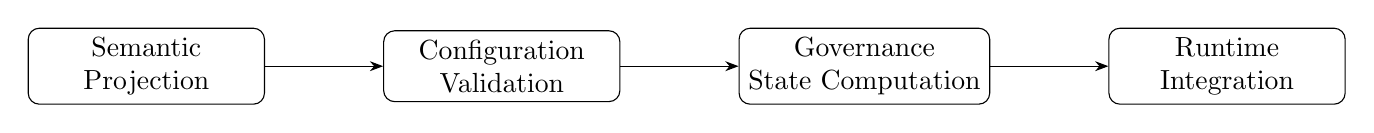
\begin{tikzpicture}[
node distance=1.5cm,
every node/.style={
draw,
rounded corners,
align=center,
minimum width=3cm,
minimum height=0.8cm
},
>=Stealth
]

\node (projection) {Semantic\\Projection};
\node (validation) [right=of projection] {Configuration\\Validation};
\node (states) [right=of validation] {Governance\\State Computation};
\node (runtime) [right=of states] {Runtime\\Integration};

\draw[->] (projection) -- (validation);
\draw[->] (validation) -- (states);
\draw[->] (states) -- (runtime);

\end{tikzpicture}

\caption{Governance processing pipeline implemented by the reference operationalization.}
\label{fig:governance_processing_pipeline}
\end{figure}

\subsubsection{Processing Stage 1: Semantic Projection}

The first processing stage transforms framework-specific configuration artifacts into ACM concepts according to the semantic projection rules introduced in Section~\ref{sec:semantic_projection}. The objective is to preserve governance-relevant semantics rather than reproduce the native internal representation of the originating framework.

\begin{algorithm}[ht]
\caption{Semantic Projection}
\KwIn{Native framework configuration $F$}
\KwOut{Projected ACM objects}

Extract native artifacts\;

Apply framework-specific projection rules\;

Create projected ACM objects\;

Preserve provenance metadata\;

\Return projected configuration\;

\end{algorithm}

The resulting representation remains independent of governance processing and serves as the input to the normalization and validation stages.

\subsubsection{Processing Stage 2: Configuration Validation}

Configuration validation verifies that the projected ACM representation satisfies the structural constraints required by the reference model before governance states are computed.

Validation is intentionally deterministic and independent of runtime execution. It verifies object identities, reference consistency, relationship integrity, digest computation, and structural constraints while preserving the immutability of validated revisions.

\begin{algorithm}[ht]
\caption{Configuration Validation}
\KwIn{Normalized ACM configuration}
\KwOut{Validated configuration}

Resolve references\;

Verify structural constraints\;

Compute canonical digests\;

Detect structural inconsistencies\;

Produce validation report\;

\Return validated configuration\;

\end{algorithm}

Only validated ACM representations are processed by the governance engine.

\subsubsection{Processing Stage 3: Governance State Computation}

Once the configuration has been validated, governance states are computed according to the formal semantics introduced in Section~\ref{sec:governance_semantics}. This stage evaluates lifecycle status, impact propagation, eligibility, and assurance until a deterministic fixed point is reached.

Unlike lifecycle states, which remain intrinsic properties of immutable revisions, computed governance states are derived from the dependency structure of the configuration graph and may therefore evolve whenever dependencies change.

\begin{algorithm}[ht]
\caption{Governance State Computation}
\KwIn{Validated ACM configuration}
\KwOut{Computed governance states}

Initialize computed states\;

Repeat

\Indp

Compute impact propagation\;

Update eligibility\;

Update assurance\;

\Indm

Until convergence\;

\Return governed configuration\;

\end{algorithm}

Because propagation is deterministic over a finite configuration graph, convergence always produces a unique governance state for a given configuration and governance policy.

\subsubsection{Processing Stage 4: Runtime Integration}

The final processing stage incorporates runtime observations into the governance model without modifying immutable configuration artifacts. Runtime signals are normalized into ACM runtime events and integrated into the Runtime Graph introduced in Section~\ref{sec:governance_semantics}.

This separation preserves the distinction between governed configurations and operational execution while enabling replay, auditing, and runtime traceability.

\begin{algorithm}[ht]
\caption{Runtime Integration}
\KwIn{Runtime events}
\KwOut{Updated Runtime Graph}

Normalize runtime events\;

Update runtime graph\;

Maintain provenance\;

Enable replay reconstruction\;

\Return runtime representation\;

\end{algorithm}

Since runtime integration operates exclusively on normalized events, the resulting Runtime Graph remains independent of the native event formats exposed by individual execution frameworks.

\subsection{Reference Implementation}
\label{sec:reference_implementation}

The ACM reference model is operationalized through an open-source Python reference implementation developed to validate the feasibility of the proposed concepts and governance semantics. The implementation is intentionally presented as a reference operationalization rather than as a production-ready governance platform. Its primary objective is to demonstrate that the reference model can be realized using deterministic processing stages while remaining independent of any particular execution framework.

The implementation follows the layered architecture introduced in Section~\ref{sec:operationalization}. Framework-specific adapters are responsible for semantic projection, whereas the governance kernel operates exclusively on normalized ACM representations. This architectural separation ensures that governance algorithms remain independent of framework-specific execution models and may therefore be reused by future adapters without modification.

The implementation organizes configuration artifacts as immutable Agentic Configuration Item (ACI) revisions represented through strongly typed data models. Canonical serialization and content-addressed digests provide stable identities for configuration revisions, enabling deterministic comparison, provenance tracking, baseline management, and reproducible replay of governed configurations.

Governance processing is implemented as a deterministic pipeline corresponding directly to the formal semantics introduced in Section~\ref{sec:governance_semantics}. Configuration validation, lifecycle management, governance state computation, and runtime integration operate on immutable configuration revisions without modifying the underlying configuration artifacts. Runtime observations are maintained separately within the Runtime Graph, preserving the conceptual distinction between governed configurations and operational execution.

The modular organization of the reference implementation also facilitates extensibility. Supporting an additional agentic framework only requires the implementation of a new semantic projection adapter capable of producing normalized ACM artifacts. Since all subsequent governance processing operates exclusively on the normalized representation, no modification of the governance kernel is required when integrating additional frameworks (see Figure ~\ref{fig:operationalization_acm}).

\begin{figure*}[t]
	\centering
	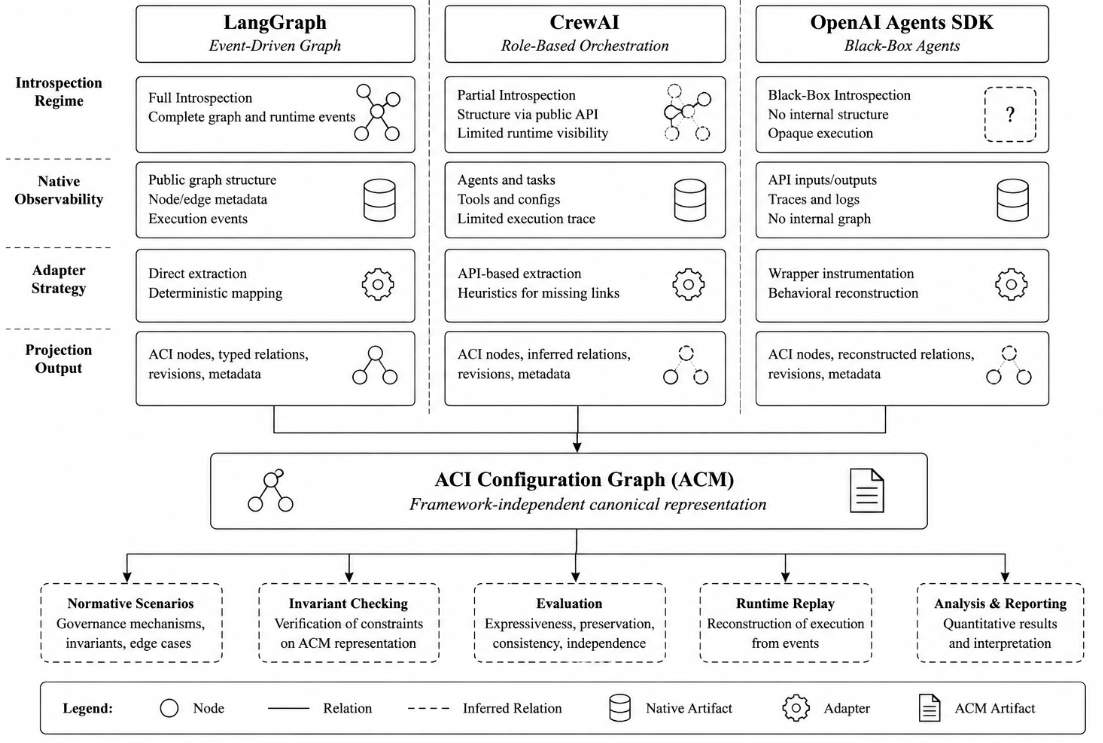
\includegraphics[width=\textwidth]{figures/operationalization_acm.png}
	\caption{Operationalization of the ACM reference model through semantic projection. Native framework configurations are projected into a common framework-independent governance representation, while a reference implementation demonstrates validation, runtime replay and conformance, and impact analysis based on the ACM governance semantics.}
	\label{fig:operationalization_acm}
\end{figure*}

Thus, the reference implementation serves as the experimental artifact supporting the evaluation presented in Section~\ref{sec:evaluation}. All normative scenarios, automated validation procedures, and cross-framework projection experiments reported in this paper are executed using this implementation, providing empirical evidence that the ACM reference model can be operationalized consistently while preserving framework-independent governance semantics. Finally, operationalization validates the implementability of the reference model; evaluation validates its expressiveness.

\begin{table}[ht]
\centering
\caption{Correspondence between ACM concepts and the reference implementation.}
\label{tab:implementation_mapping}
\begin{tabular}{ll}
\toprule
\textbf{ACM Concept} & \textbf{Reference Implementation} \\
\midrule
Reference Model & Strongly typed ACI data models \\
Semantic Projection & Framework adapters \\
Governance Processing & Deterministic governance kernel \\
Configuration Graphs & Canonical graph representations \\
Runtime Semantics & Runtime event normalization \\
Reference Operationalization & Python implementation \\
\bottomrule
\end{tabular}
\end{table}

The Figure ~\ref{fig:aci_metamodel_implementation} depicts the UML representation of an ACI object in the reference implementation.

\begin{figure*}[t]
	\centering
	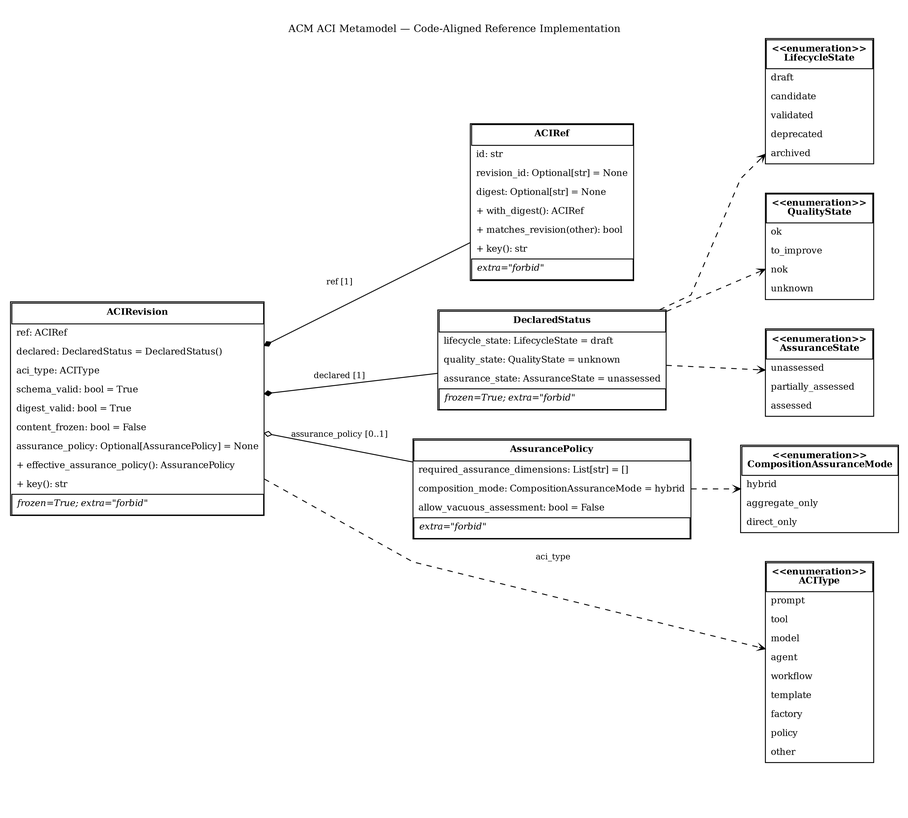
\includegraphics[width=\textwidth]{figures/ACI_metamodel.png}
	\caption{UML representation of the core ACIRevision model in the ACM reference implementation. The diagram shows the immutable ACIRevision object together with its references, declared governance state, assurance policy, and associated enumerations, providing the structural basis of the reference implementation.}
	\label{fig:aci_metamodel_implementation}
\end{figure*}

\section{Evaluation}
\label{sec:evaluation}

The previous section demonstrated how the ACM reference model can be operationalized through a framework-independent governance architecture, semantic projection pipeline, and reference implementation. The remaining question is whether this operationalization effectively preserves the governance semantics defined by the reference model while supporting heterogeneous agentic frameworks in practice.

The objective of this evaluation is therefore not to benchmark execution performance or compare orchestration frameworks. Instead, it assesses the extent to which the ACM reference model provides a consistent and operational foundation for configuration governance across heterogeneous agentic systems. More specifically, the evaluation investigates whether configurations originating from different frameworks can be projected into a common representation while preserving governance-relevant semantics and enabling deterministic governance processing.

The evaluation is conducted using the Python reference implementation presented in Section~\ref{sec:operationalization}. Two representative agentic frameworks, LangGraph and CrewAI, are used as experimental case studies because they embody distinct orchestration paradigms while remaining sufficiently mature and widely adopted within the current agentic ecosystem. The experimental protocol combines semantic projection experiments, normative governance scenarios, automated validation procedures, and runtime integration experiments in order to assess the operational feasibility of the proposed reference model.

The remainder of this section is organized as follows. Section~7.1 introduces the research questions guiding the evaluation. Section~7.2 describes the experimental methodology. Section~7.3 presents the experimental results, while Section~7.4 discusses their implications with respect to the objectives of the ACM reference model.

\subsection{Evaluation Objectives}
\label{sec:evaluation_objectives}

The evaluation aims to determine whether the ACM reference model fulfills the objectives defined throughout this paper. Rather than evaluating implementation-specific characteristics, the experiments focus on validating the conceptual properties of the reference model, its governance semantics, and its ability to provide a common governance layer across heterogeneous agentic frameworks.

To structure the evaluation, four research questions are defined.

\begin{itemize}

\item \textbf{RQ1 -- Expressiveness.}
Can the ACM reference model represent heterogeneous agentic configurations originating from different orchestration frameworks using a common governance representation?

\item \textbf{RQ2 -- Governance Preservation.}
Does semantic projection preserve the governance-relevant semantics of native configurations, including configuration identity, provenance, dependency relationships, lifecycle information, and runtime traceability?

\item \textbf{RQ3 -- Operational Feasibility.}
Can the governance semantics introduced in this paper be operationalized through a deterministic processing pipeline supporting configuration validation, governance state computation, and runtime integration?

\item \textbf{RQ4 -- Framework Independence.}
Can identical governance mechanisms be applied to configurations originating from structurally different frameworks without modifying the governance kernel?

\end{itemize}

These research questions directly reflect the principal design objectives introduced in Sections~3--6. Consequently, the evaluation does not attempt to compare the execution capabilities of individual agentic frameworks. Instead, it investigates whether ACM succeeds in abstracting framework-specific configuration models into a unified governance representation while preserving the semantics required for configuration management.

The following sections describe the experimental methodology adopted to answer these research questions and present the empirical evidence collected using the reference implementation.

\begin{table}[ht]
\centering
\caption{Research questions and evaluation criteria.}
\label{tab:research_questions}
\begin{tabular}{p{1cm} p{4.6cm} p{5.8cm}}
\toprule
\textbf{RQ} & \textbf{Objective} & \textbf{Evaluation Evidence} \\
\midrule
RQ1 & Assess the expressiveness of the ACM representation & Cross-framework semantic projection \\
RQ2 & Assess governance semantics preservation & Projection outcome analysis and governance validation \\
RQ3 & Assess operational feasibility & Automated governance scenarios and deterministic processing \\
RQ4 & Assess framework independence & Cross-framework execution of identical governance mechanisms \\
\bottomrule
\end{tabular}
\end{table}
\subsection{Experimental Methodology}
\label{sec:evaluation_methodology}

The experimental methodology was designed to evaluate the ACM reference model with respect to the research questions introduced in Section~\ref{sec:evaluation_objectives}. Rather than measuring execution performance, the experiments assess whether heterogeneous agentic configurations can be governed through a common configuration model while preserving the governance semantics defined throughout this paper.

All experiments were conducted using the Python reference implementation described in Section~\ref{sec:reference_implementation}. This implementation realizes the semantic projection pipeline, governance processing stages, and runtime integration mechanisms introduced in Section~\ref{sec:operationalization}. It serves exclusively as an experimental artifact supporting the evaluation of the reference model.

Two representative agentic frameworks were selected as experimental case studies:

\begin{itemize}
\item \textbf{LangGraph}, representing explicit graph-based orchestration;
\item \textbf{CrewAI}, representing declarative agent-task orchestration.
\end{itemize}

These frameworks were intentionally chosen because they rely on different orchestration abstractions while exposing sufficiently rich configuration models to evaluate the framework-independence of ACM.

The evaluation combines four complementary experimental activities:

\begin{enumerate}

\item semantic projection of native framework configurations into normalized ACM representations;

\item execution of normative governance scenarios covering lifecycle management, dependency propagation, assurance evaluation, and runtime semantics;

\item automated validation of governance invariants and deterministic processing through the reference implementation;

\item comparative analysis of governance behavior across both frameworks.

\end{enumerate}

This methodology provides complementary evidence regarding both the conceptual validity of the ACM reference model and its practical operationalization. While semantic projection evaluates the expressiveness of the reference model, the governance scenarios validate the formal semantics introduced in Section~\ref{sec:governance_semantics}. Automated validation ensures that governance processing remains deterministic and reproducible, whereas the comparative analysis assesses the framework independence of the proposed governance architecture.

\begin{table}[ht]
\centering
\caption{Experimental protocol used to evaluate the ACM reference model.}
\label{tab:experimental_protocol}

\begin{tabular}{p{3.8cm}p{3.8cm}p{4.4cm}}
\toprule
\textbf{Experimental Activity} &
\textbf{Objective} &
\textbf{Research Questions} \\
\midrule

Semantic Projection &
Evaluate representational expressiveness &
RQ1, RQ2 \\

Governance Scenarios &
Validate governance semantics &
RQ2, RQ3 \\

Automated Validation &
Verify deterministic governance processing &
RQ3 \\

Cross-framework Comparison &
Assess framework independence &
RQ1, RQ4 \\

\bottomrule
\end{tabular}

\end{table}

\begin{figure}[ht]
\centering

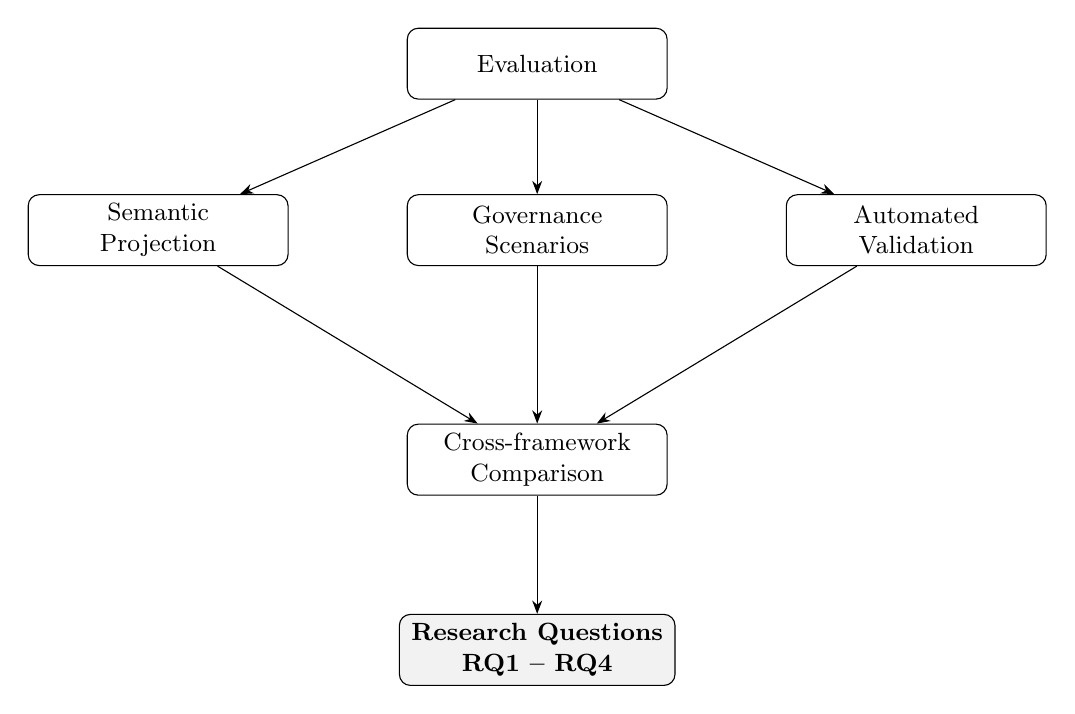
\begin{tikzpicture}[
node distance=1.2cm and 1.5cm,
>=Stealth,
process/.style={
draw,
rounded corners,
align=center,
minimum width=3.3cm,
minimum height=0.9cm,
font=\small
},
rq/.style={
draw,
rounded corners,
fill=gray!10,
align=center,
minimum width=3.5cm,
minimum height=0.9cm,
font=\small\bfseries
}
]

% Top
\node[process] (eval) {Evaluation};

% Middle row
\node[process, below left=of eval] (projection) {Semantic\\Projection};

\node[process, below=of eval] (scenarios) {Governance\\Scenarios};

\node[process, below right=of eval] (validation) {Automated\\Validation};

% Comparison
\node[process, below=2.0cm of scenarios] (comparison)
{Cross-framework\\Comparison};

% Bottom
\node[rq, below=1.5cm of comparison]
(rqs)
{Research Questions\\RQ1 -- RQ4};

% Connections
\draw[->] (eval) -- (projection);
\draw[->] (eval) -- (scenarios);
\draw[->] (eval) -- (validation);

\draw[->] (projection) -- (comparison);
\draw[->] (scenarios) -- (comparison);
\draw[->] (validation) -- (comparison);

\draw[->] (comparison) -- (rqs);

\end{tikzpicture}

\caption{Experimental methodology adopted to evaluate the ACM reference model. Complementary experimental activities collectively provide evidence for answering the research questions.}

\label{fig:evaluation_methodology}

\end{figure}

\subsection{Evaluation Results}
\label{sec:experimental_results}

This section presents the experimental evidence collected using the methodology described in Section~\ref{sec:experimental_methodology}. The objective is not to evaluate execution performance, but to assess whether the ACM reference model satisfies the research questions introduced in Section~\ref{sec:evaluation_objectives}. The reported results are derived from the latest validation and preservation reports generated by the reference implementation.

The evaluation addresses four complementary dimensions: (i) the representational expressiveness of ACM, (ii) the preservation of governance semantics during semantic projection, (iii) the deterministic operationalization of the governance model, and (iv) the framework-independent behavior of the governance kernel.

%%%%%%%%%%%%%%%%%%%%%%%%%%%%%%%%%%%%%%%%%%%%%%%%%%%%%%%%%%%%%%%%%%%%%%%%%%%%%%%%
\subsubsection{Model Expressiveness}
\label{subsubsec:model_expressiveness}

The first research question investigates whether ACM provides a sufficiently
expressive configuration model to represent heterogeneous agentic systems while
preserving the governance information required for lifecycle management,
traceability, and runtime conformance.

Unlike programming languages, where expressiveness is often associated with the
set of computable behaviors, the notion of expressiveness considered in this
work refers to the ability of the reference model to faithfully represent the
configuration semantics of an existing agentic framework.

Accordingly, the expressiveness of ACM is operationalized through three
complementary dimensions:

\begin{enumerate}
	\item \textbf{Configuration Coverage}, measuring how many native
	configuration constructs can be represented by ACM;
	\item \textbf{Semantic Preservation}, measuring whether the governance
	meaning of supported constructs is preserved after projection;
	\item \textbf{Information Loss}, measuring the proportion of native
	information that cannot be represented by the current reference
	model.
\end{enumerate}

These dimensions provide a quantitative characterization of expressiveness that
can be reproduced independently of the implementation (see Appendix ~\ref{appendix:evaluation_semantics}). The related Research Questions and their evaluation are presented in Table ~\ref{tab:evaluation_metrics}.

\begin{table}[t]
	\centering
	\caption{Relationship between evaluation metrics and experimental evidence.}
	\label{tab:evaluation_metrics}
	\renewcommand{\arraystretch}{1.2}
	\begin{tabularx}{\linewidth}{lXX}
		\toprule
		\textbf{Metric} &
		\textbf{Primary Evaluation Method} &
		\textbf{Purpose} \\
		\midrule
		
		Configuration Coverage &
		Semantic projection experiments (LangGraph and CrewAI) &
		Assess whether governance-relevant native constructs can be represented by the ACM reference model. \\
		
		Semantic Preservation (Expressiveness) &
		Preservation analysis and normative scenarios &
		Assess whether the governance semantics of projected configurations are preserved and satisfy the expected ACM invariants. \\
		
		Information Loss &
		Preservation reports generated during semantic projection &
		Identify and characterize governance-relevant information that cannot currently be represented or must be approximated by the reference model. \\
		
		\bottomrule
	\end{tabularx}
\end{table}

\paragraph{Overall Expressiveness}

The three previous metrics characterize complementary aspects of model
expressiveness.

Configuration Coverage evaluates representational completeness, Semantic
Preservation evaluates governance fidelity, and Information Loss quantifies the
remaining limitations of the current reference model.

Rather than combining these dimensions into a single weighted score, they are
reported independently throughout the evaluation. This choice preserves their
interpretability and avoids introducing arbitrary weighting factors that would
depend on the characteristics of individual frameworks.


\subsubsection{Governance Semantics Preservation}

A principal objective of semantic projection is the preservation of governance-relevant semantics rather than the exact reproduction of native framework implementations.

According to the preservation reports, both evaluated adapters preserve all structural elements within the normative ACM scope. Nodes, structural relationships, workflow branches, entry points, terminal nodes, prompt references, tool references, and canonical configuration digests are preserved for the evaluated workflows. Repeated projections produce identical canonical digests, demonstrating deterministic normalization.

The only remaining approximations concern execution semantics that are intentionally opaque to the native frameworks themselves. In particular, conditional routing logic implemented through arbitrary Python functions cannot be reconstructed statically and is therefore represented as an abstract routing structure. Likewise, CrewAI Flow state schemas currently remain outside the normative ACM scope and are consequently classified as unsupported rather than reconstructed.

Importantly, these limitations affect execution-specific implementation details rather than the governance semantics required by ACM. Configuration identity, provenance, dependency relationships, lifecycle information, runtime traceability, and configuration validation remain fully preserved throughout the projection process.

\begin{table}[ht]
\centering
\caption{Governance semantics preservation for the evaluated workflows.}
\label{tab:preservation_summary}

\begin{tabular}{lccc}
\toprule
\textbf{Governance Property} &
\textbf{Preserved} &
\textbf{Approximated} &
\textbf{Unsupported} \\
\midrule
Configuration identity & \checkmark & - & - \\
Revision provenance & \checkmark & - & - \\
Dependency graph & \checkmark & - & - \\
Prompt references & \checkmark & - & - \\
Tool references & \checkmark & - & - \\
Canonical digests & \checkmark & - & - \\
Conditional routing semantics & - & \checkmark & - \\
Framework-specific runtime state & - & - & \checkmark \\
\bottomrule
\end{tabular}

\end{table}

%%%%%%%%%%%%%%%%%%%%%%%%%%%%%%%%%%%%%%%%%%%%%%%%%%%%%%%%%%%%%%%%%%%%%%%%%%%%%%%%
\subsubsection{Operational Results}
\label{subsubsec:operational_results}

The reference implementation was evaluated using the complete experimental
protocol described previously. The evaluation combined declarative fixtures,
dedicated scenario-specific tests, framework adapters, runtime validation, and
benchmark experiments (Complete scenarios description in Appendix ~\ref{appendix:configuration_baseline}).

Overall, the evaluation successfully completed the complete normative scenario
suite without unresolved implementation inconsistencies after the final
refinements of the governance kernel. The resulting experimental campaign
covered all fourteen normative invariants introduced in
Section~\ref{sec:governance_semantics} and exercised the principal governance
mechanisms of the reference model.

Table~\ref{tab:scenario_results} summarizes the execution results obtained for
the twenty-seven evaluation scenarios.

\begin{table}[t]
\caption{Summary of operational evaluation results.}
\label{tab:scenario_results}
\centering
\begin{tabular}{lc}
\hline
Metric & Result\\
\hline
Normative scenarios & 27\\
Declarative fixtures & 11\\
Normative invariants evaluated & 14\\
Automated tests passed & 221\\
Automated tests skipped & 3\\
Kernel inconsistencies requiring refinement & 2\\
\hline
\end{tabular}
\end{table}

Beyond the numerical results, the evaluation provides several observations that
directly address the research questions introduced in
Section~\ref{sec:evaluation_methodology}.

\paragraph{Contribution to RQ1 (Model Expressiveness).}

These results provide positive evidence for \textbf{RQ1}. They show that ACM is sufficiently expressive to capture the governance-relevant configuration concepts of the evaluated agentic systems while preserving the information required for lifecycle management, dependency modeling, provenance, runtime traceability, and governance evaluation. Importantly, framework-specific constructs that cannot yet be represented are explicitly reported during semantic projection rather than silently discarded, making the current boundaries of the reference model transparent and enabling controlled future extensions.

\paragraph{Contribution to RQ2 (Semantic Preservation).}

These results provide positive evidence for \textbf{RQ2}. They indicate that the governance semantics defined by ACM are preserved throughout the semantic projection process (defined in
Section~\ref{sec:governance_semantics} and in Appendix ~\ref{appendix:projection_formalism}) including lifecycle transitions, dependency propagation, assurance evaluation, eligibility computation, runtime traceability, and drift detection. The deterministic replay experiments further demonstrate that governance states can be reconstructed reproducibly from normalized runtime events independently of probabilistic LLM outputs. The discrepancies initially identified in scenarios ACM-S02 and ACM-S20 led to normative refinements of the reference implementation, illustrating the effectiveness of the scenario-based validation methodology in strengthening the consistency between the formal specification and its operational realization.

\paragraph{Contribution to RQ3 (Framework Independence).}

These results provide positive evidence for \textbf{RQ3}. They demonstrate that governance-relevant configurations originating from structurally different orchestration frameworks can be projected into a common ACM representation while preserving the governance semantics required for lifecycle management, provenance, dependency analysis, and runtime governance. The consistent behavior of semantic projection and runtime normalization across the evaluated scenarios further supports the framework-independent design objective of ACM. These findings should nevertheless be interpreted within the scope of the present study: they demonstrate the feasibility of normalizing representative configurations from two complementary orchestration paradigms rather than universal compatibility with all existing or future agentic frameworks.

\paragraph{Overall Interpretation.}

Taken together, the operational results indicate that the reference
implementation faithfully operationalizes the proposed governance semantics and
that the experimental protocol is sufficiently comprehensive to evaluate the
principal properties of the ACM reference model. Rather than merely
demonstrating software correctness, the evaluation provides empirical evidence
that the concepts introduced by ACM are internally consistent, reproducible,
and applicable across heterogeneous agentic configurations within the scope of
the evaluated frameworks.

%%%%%%%%%%%%%%%%%%%%%%%%%%%%%%%%%%%%%%%%%%%%%%%%%%%%%%%%%%%%%%%%%%%%%%%%%%%%%%%%
\subsection{Discussion of Results}
\label{subsec:discussion_results}

The experimental evaluation provides evidence that the proposed ACM reference
model constitutes a coherent governance abstraction for agentic systems. Beyond
the individual research questions addressed in the previous subsections, several
broader observations emerge from the evaluation.

First, the scenario-based validation demonstrates that governance can be
specified independently of execution frameworks. Throughout the experimental
campaign, the same governance semantics were successfully applied to different
orchestration paradigms after semantic projection into the ACM reference model.
This separation between implementation-specific execution and
framework-independent governance is one of the principal architectural
contributions of ACM.

Second, the evaluation confirms the importance of treating configuration as an
immutable governance artifact rather than as a mutable runtime object.
Lifecycle transitions, assurance propagation, dependency analysis, runtime
traceability, and deterministic replay all rely on immutable revisions whose
identities remain stable throughout the system lifecycle. This design enables
governance decisions to be reproduced and audited independently of the
probabilistic behavior of the underlying language models.

Third, the experimental campaign illustrates the value of formal governance
semantics. Rather than serving solely as theoretical specifications, the
normative invariants provided an executable contract against which the reference
implementation could be continuously validated. The two implementation
discrepancies identified during the evaluation (ACM-S02 and ACM-S20) were not
limitations of the methodology but evidence of its effectiveness in revealing
ambiguities requiring refinement of the governance kernel. The final model
therefore benefits directly from the iterative interaction between formal
specification and implementation.

The evaluation highlights the current scope of ACM. The experiments
demonstrate that the proposed governance semantics are applicable across the
representative orchestration frameworks considered in this work while remaining
computationally practical for the evaluated configuration sizes. At the same
time, the study intentionally does not claim universal framework compatibility
or enterprise-scale validation. These aspects constitute natural directions for
future extensions of the reference model.

Overall, the results support the central hypothesis of this work: governance of
agentic systems can be modeled independently from execution frameworks through
an immutable configuration model, explicit lifecycle semantics, deterministic
governance propagation, and runtime traceability. The consistency observed
across the complete evaluation campaign suggests that ACM provides a sound
foundation upon which richer governance capabilities can be developed in future
work.

\begin{table}[ht]

\centering

\caption{Summary of research question outcomes.}

\label{tab:rq_summary}

\begin{tabular}{p{1cm}p{2.7cm}p{5cm}p{2cm}}

\toprule

\textbf{RQ} &
\textbf{Objective} &
\textbf{Evidence} &
\textbf{Outcome}

\\

\midrule

RQ1 &
Expressiveness &
Successful cross-framework representation &
Supported

\\

RQ2 &
Governance preservation &
Semantic preservation analysis &
Supported

\\

RQ3 &
Operational feasibility &
Automated validation and deterministic processing &
Supported

\\

RQ4 &
Framework independence &
Identical governance processing across frameworks &
Supported within evaluated scope

\\

\bottomrule

\end{tabular}

\end{table}

\section{Discussion}
\label{sec:discussion}
\subsection{Positioning with Respect to Existing Agentic Frameworks}
\label{sec:positioning}

The rapid emergence of agentic frameworks has significantly simplified the development of LLM-based applications by providing increasingly sophisticated abstractions for workflow orchestration, agent coordination, tool integration, and execution management. Frameworks such as LangGraph and CrewAI exemplify this evolution by exposing distinct orchestration paradigms tailored to different classes of agentic systems.

The objective of ACM is fundamentally different. Rather than providing execution capabilities, ACM introduces a framework-independent governance layer dedicated to the management of agentic configurations throughout their lifecycle. Consequently, ACM should not be interpreted as an alternative orchestration framework, but as a complementary governance model capable of operating across heterogeneous execution environments.

This distinction is reflected in the responsibilities addressed by each approach. Agentic frameworks primarily define how agents execute, communicate, and coordinate during runtime. ACM, by contrast, governs what is being executed by providing immutable configuration revisions, provenance tracking, lifecycle management, dependency analysis, baseline management, assurance evaluation, and runtime traceability. Execution and governance therefore constitute complementary concerns operating at different abstraction levels.

The semantic projection mechanism provides the interface between these two layers (see Appendix ~\ref{appendix:projection_formalism}). By translating framework-specific configurations into normalized ACM artifacts, governance processing becomes independent of the originating execution framework while preserving the governance semantics required for configuration management. This separation allows identical governance mechanisms to be applied to configurations originating from heterogeneous orchestration paradigms without introducing framework-specific logic into the governance kernel.

More generally, the proposed architecture aligns with the long-established separation between execution infrastructures and configuration management observed in traditional software engineering. Source code management systems, build systems, deployment platforms, and runtime environments have historically evolved as complementary but distinct components of the software lifecycle \cite{ref25}. ACM extends this principle to agentic systems by introducing an explicit governance layer dedicated to the management of agentic configurations rather than their execution.

The experimental evaluation presented in Section~\ref{sec:evaluation} provides initial evidence supporting this positioning. The successful projection of representative LangGraph and CrewAI workflows into a common ACM representation demonstrates that governance can be decoupled from execution while preserving the semantics required for configuration management. Although the current evaluation remains limited to two representative frameworks, the obtained results suggest that this architectural separation provides a viable foundation for framework-independent governance of agentic systems.

\begin{figure}[t]
    \centering

    \begin{tikzpicture}[
        font=\scriptsize,
        node distance=4mm and 3mm,
        layer/.style={
            draw,
            rounded corners=1.5pt,
            minimum width=0.94\columnwidth,
            inner xsep=4pt,
            inner ysep=5pt,
            align=center,
            line width=0.6pt
        },
        component/.style={
            draw,
            rounded corners=1pt,
            minimum height=6mm,
            inner xsep=4pt,
            inner ysep=2pt,
            align=center,
            line width=0.45pt
        },
        projection/.style={
            draw,
            minimum width=0.58\columnwidth,
            minimum height=6mm,
            align=center,
            line width=0.6pt
        },
        arrow/.style={
            -{Latex[length=2mm,width=1.3mm]},
            line width=0.65pt
        }
    ]

    % ---------------------------------------------------------
    % Execution layer
    % ---------------------------------------------------------

    \node[layer] (execution) {
        \textbf{Agentic Execution Frameworks}\\[4pt]
        \begin{tikzpicture}[
            baseline,
            component/.style={
                draw,
                rounded corners=1pt,
                minimum width=21mm,
                minimum height=6mm,
                align=center,
                line width=0.45pt
            }
        ]
            \node[component] (langgraph) {LangGraph};
            \node[component, right=2mm of langgraph] (crewai) {CrewAI};
            \node[component, right=2mm of crewai] (others) {Other Frameworks};
        \end{tikzpicture}
    };

    % ---------------------------------------------------------
    % Semantic projection
    % ---------------------------------------------------------

    \node[projection, below=5mm of execution] (projection) {
        \textbf{Semantic Projection}\\
        Framework-specific adapter and normalization
    };

    \draw[arrow] (execution) -- (projection);

    % ---------------------------------------------------------
    % ACM governance layer
    % ---------------------------------------------------------

    \node[layer, below=5mm of projection] (acm) {
        \textbf{ACM Framework-Independent Governance Layer}\\[4pt]
        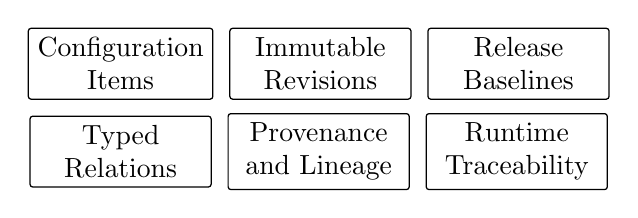
\begin{tikzpicture}[
            baseline,
            component/.style={
                draw,
                rounded corners=1pt,
                minimum width=23mm,
                minimum height=6mm,
                align=center,
                line width=0.45pt
            }
        ]
            \node[component] (aci) {Configuration\\Items};
            \node[component, right=2mm of aci] (revisions) {Immutable\\Revisions};
            \node[component, right=2mm of revisions] (baselines) {Release\\Baselines};

            \node[component, below=2mm of aci] (relations) {Typed\\Relations};
            \node[component, right=2mm of relations] (provenance) {Provenance\\and Lineage};
            \node[component, right=2mm of provenance] (runtime) {Runtime\\Traceability};
        \end{tikzpicture}
    };

    \draw[arrow] (projection) -- (acm);

    % ---------------------------------------------------------
    % Governance capabilities
    % ---------------------------------------------------------

    \node[layer, below=5mm of acm] (governance) {
        \textbf{Governance Capabilities}\\[4pt]
        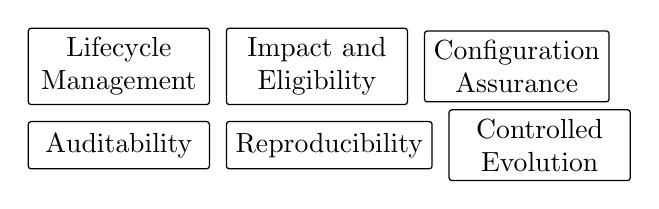
\begin{tikzpicture}[
            baseline,
            component/.style={
                draw,
                rounded corners=1pt,
                minimum width=23mm,
                minimum height=6mm,
                align=center,
                line width=0.45pt
            }
        ]
            \node[component] (lifecycle) {Lifecycle\\Management};
            \node[component, right=2mm of lifecycle] (impact) {Impact and\\Eligibility};
            \node[component, right=2mm of impact] (assurance) {Configuration\\Assurance};

            \node[component, below=2mm of lifecycle] (audit) {Auditability};
            \node[component, right=2mm of audit] (reproducibility) {Reproducibility};
            \node[component, right=2mm of reproducibility] (change) {Controlled\\Evolution};
        \end{tikzpicture}
    };

    \draw[arrow] (acm) -- (governance);

    \end{tikzpicture}

    \caption{Positioning of ACM with respect to agentic execution frameworks. Framework-specific configurations are semantically projected into a common governance representation, allowing lifecycle, assurance, traceability, and change-management mechanisms to operate independently of the originating framework.}
    \label{fig:acm_framework_positioning}
\end{figure}

\subsection{Contributions to Agentic Configuration Governance}
\label{sec:governance_contributions}

The contribution of ACM lies neither in introducing a new orchestration mechanism nor in extending the execution capabilities of existing agentic frameworks. Its primary contribution is to establish configuration governance as an explicit and framework-independent concern for agentic systems. From this perspective, ACM contributes at four complementary levels: representation, semantics, interoperability, and operational validation.

\subsubsection{A Framework-Independent Governance Representation}

The first contribution is a reference model that represents an agentic system as a governed configuration rather than as a collection of framework-specific runtime objects. The model introduces explicit configuration items, immutable revisions, typed relationships, provenance information, and release baselines. These abstractions provide a common vocabulary for describing the constituent elements of an agentic system and the dependencies that determine its effective configuration.

This representation extends established configuration-management principles to artifacts that are specific to agentic systems. In particular, it treats agents, prompts, tools, policies, models, workflows, and dynamically instantiated components as governable objects whose identity and evolution can be tracked independently. The resulting configuration is therefore not reduced to source code, deployment metadata, or execution traces. It is represented as an explicit and auditable object in its own right.

A central consequence of this model is the ability to distinguish logical identity from immutable revision identity. Successive revisions of the same configuration item preserve a stable conceptual identity while remaining individually addressable through exact revision identifiers and content digests. This distinction supports reproducibility, comparison, controlled replacement, and historical reconstruction without conflating an evolving artifact with one of its concrete states.

\subsubsection{Formal Governance Semantics}

The second contribution is the formalization of governance semantics over the reference model. ACM does not merely describe which artifacts exist; it defines how their governance states evolve and how local changes affect dependent configurations.

The lifecycle model specifies admissible transitions for configuration revisions, baselines, and runtime instances. Quality, assurance, impact, and eligibility are maintained as distinct dimensions rather than being collapsed into a single status. This separation prevents ambiguous interpretations such as treating a lack of evidence as proof of poor quality or propagating the lifecycle state of a dependency directly to its parent.

The propagation semantics further define how dependency changes, invalidated evidence, deprecated components, and runtime deviations influence the governance status of composite configurations. These effects are restrictive rather than destructive: a problematic dependency may block the promotion of a composite configuration without rewriting the intrinsic quality or lifecycle state of that composite. The model thereby preserves the provenance of governance decisions while supporting deterministic and explainable state computation.

The assurance model complements these semantics by linking governance conclusions to explicit evidence. Validation and approval are attached to exact revisions and scopes, allowing the system to distinguish directly assessed artifacts from conclusions inherited through assurance-relevant dependencies. Governance states can therefore be interpreted together with the evidence and rules from which they were derived.

\subsubsection{Framework-Independent Semantic Projection}

The third contribution is the separation between framework-specific extraction and framework-independent governance processing. Native configurations are translated into ACM through semantic projection, while the governance kernel operates exclusively on normalized ACM artifacts.

This architecture allows heterogeneous orchestration paradigms to be governed through a common representation. A graph-oriented framework may expose nodes and edges directly, whereas a role- and task-oriented framework may require part of its topology to be reconstructed from assignments and dependencies. ACM does not require these native representations to be structurally identical. It requires the projection to preserve the information needed for configuration governance and to make approximated or unavailable information explicit.

Framework independence should therefore be understood as independence of the governance model and processing semantics from a specific execution framework. The adapters remain framework-specific because they interpret native concepts. Once projection is complete, however, lifecycle validation, baseline construction, dependency analysis, assurance computation, runtime integration, and impact propagation no longer depend on the source framework.

This separation provides a basis for interoperability without imposing a common execution model. Frameworks retain their native orchestration semantics, while ACM supplies a shared governance representation above them.

\subsubsection{Reference Operationalization and Evaluation}

The fourth contribution is the operationalization of the reference model through an executable implementation and its evaluation across two distinct agentic frameworks. The Python prototype demonstrates that the proposed abstractions and semantics can be implemented as deterministic processing mechanisms rather than remaining solely conceptual definitions.

The reference implementation operationalizes immutable revisions, canonical serialization, configuration validation, state propagation, baseline processing, runtime-event normalization, and replay. The LangGraph and CrewAI adapters instantiate the semantic-projection boundary for two frameworks with different native abstractions. Their use does not establish universal applicability, but provides initial evidence that the model can accommodate both explicit graph structures and role--task compositions.

The evaluation also contributes a structured validation methodology combining normative governance scenarios, automated tests, and semantic-preservation analysis. This methodology distinguishes successful representation from exact structural equivalence and records which governance-relevant properties are preserved, reconstructed, approximated, or unavailable. It therefore provides a more appropriate validation criterion for a reference model than conventional runtime-performance benchmarking.

Taken together, these four contributions establish ACM as a configuration-governance abstraction positioned between agentic execution environments and higher-level operational or organizational governance processes. The reference model defines what is governed, the formal semantics define how governance states are computed, semantic projection connects heterogeneous frameworks to the model, and the reference implementation demonstrates that these mechanisms can be operationalized consistently.

\subsection{Practical Implications}
\label{sec:practical_implications}

Beyond its conceptual contribution, ACM has practical implications for the engineering and governance of agentic systems. By introducing an explicit and framework-independent configuration representation, the proposed model enables governance activities that are difficult to perform when configuration information remains fragmented across framework-specific abstractions.

A first implication concerns reproducibility. In current agentic ecosystems, reproducing a previous execution often requires reconstructing configurations from multiple heterogeneous artifacts, including prompts, workflow definitions, deployment parameters, runtime traces, and external resources. ACM addresses this fragmentation by associating executions with immutable configuration revisions and controlled release baselines. A governed execution can therefore be traced back to the exact configuration from which it originated, supporting reproducible experiments, regression analyses, and long-term maintenance.

A second implication concerns auditability and traceability. Since governance decisions are explicitly linked to identified configuration revisions and supporting evidence, the provenance of a validation result or lifecycle transition becomes inspectable rather than implicit. This capability facilitates post-deployment analysis, compliance reporting, and forensic investigation by making configuration evolution transparent throughout the lifecycle of the system.

The explicit representation of dependencies also supports systematic change management. Instead of reasoning independently about prompts, agents, tools, or models, ACM represents these artifacts as interconnected configuration items whose relationships can be analyzed before modifications are promoted to a released baseline. Dependency-aware impact analysis provides early visibility into the potential consequences of configuration changes, reducing the likelihood of unintended regressions.

The proposed model also provides a common governance abstraction that may facilitate interoperability across heterogeneous execution environments. Organizations frequently combine multiple orchestration frameworks to address different operational requirements. By projecting these heterogeneous configurations into a shared governance representation, ACM enables governance policies to be expressed independently of the underlying execution technology while allowing each framework to preserve its native execution semantics.

ACM may therefore contribute to the emerging AgentOps ecosystem by complementing existing observability and orchestration platforms with explicit configuration governance. Current operational platforms primarily focus on execution monitoring, tracing, evaluation, and operational metrics. ACM addresses a complementary concern by governing the configuration artifacts that determine how those executions are produced. Consequently, the model should be viewed as a governance layer that can coexist with, rather than replace, existing AgentOps and LLMOps infrastructures.

%%%%%%%%%%%%%%%%%%%%%%%%%%%%%%%%%%%%%%%%%%%%%%%%%%%%%%%%%%%%%%%%%%%%%%%%%%%%%%%%
\subsection{Limitations of the Current Reference Model}
\label{subsec:limitations}

The objective of ACM is to provide a framework-independent governance representation for the governance of agentic system configurations rather than an execution platform or an autonomous reasoning architecture. Accordingly, the current version focuses on representing governed configuration artifacts, their lifecycle, dependencies, provenance, assurance, and runtime conformance, while intentionally leaving the internal execution logic of agentic systems outside the scope of the reference model.

Table~\ref{tab:limitations_scope} summarizes the current coverage of ACM and the principal capabilities intentionally deferred to future work.

\begin{table}[t]
	\caption{Current scope of the ACM reference model.}
	\label{tab:limitations_scope}
	\centering
	\begin{tabular}{p{3.1cm}p{3.4cm}}
		\hline
		\textbf{Currently covered} &
		\textbf{Not yet covered} \\
		\hline
		Semantic projection &
		Distributed execution \\
		Configuration governance &
		Multi-agent planning strategies \\
		Immutable revision management &
		Learning and adaptation mechanisms \\
		Lifecycle semantics &
		Autonomous reasoning policies \\
		Dependency propagation &
		Self-modifying execution strategies \\
		Runtime provenance &
		Collective agent negotiation \\
		Assurance evaluation &
		Long-term memory management \\
		Deterministic replay &
		Continual learning \\
		\hline
	\end{tabular}
\end{table}

These limitations result from deliberate modeling decisions rather than technical constraints. ACM intentionally separates governance concerns from execution concerns in order to establish a stable and framework-independent governance layer. Integrating planning algorithms, reasoning strategies, learning mechanisms, or execution optimizations into the reference model would both increase its complexity and compromise the conceptual independence required for long-term interoperability.

Consequently, ACM treats reasoning engines, orchestration frameworks, planning modules, learning components, communication protocols, and other execution technologies as external systems whose observable configuration and runtime behavior can be represented and governed without prescribing their internal operation. ACM therefore specifies \emph{what} is governed---configuration revisions, baselines, dependencies, runtime observations, and assurance evidence---rather than \emph{how} autonomous agents reason, plan, negotiate, or learn.

This separation also preserves the stability of the governance model as agentic technologies evolve. New execution frameworks, orchestration paradigms, communication protocols, or reasoning techniques can be incorporated through semantic projection without modifying the governance semantics themselves. The evaluation presented in this paper should therefore be interpreted as validating the ability of ACM to represent and govern heterogeneous agentic configurations, not the correctness, efficiency, or intelligence of the underlying execution mechanisms.

The experimental validation remains limited to the representative orchestration frameworks and configuration scales considered by the reference implementation. Although the reported results provide encouraging evidence regarding the generality of the proposed governance semantics, additional empirical validation across larger industrial deployments, additional execution frameworks, and emerging agentic ecosystems will be required before broader generalization can be claimed.

\subsection{Section Summary}

This discussion has positioned ACM as a framework-independent governance representation dedicated to the governance of agentic system configurations. Rather than introducing a new execution framework, orchestration engine, or reasoning architecture, ACM provides a common semantic foundation for representing, governing, and auditing heterogeneous agentic configurations throughout their lifecycle.

The proposed reference model combines a unified configuration representation with formal governance semantics and a framework-independent operationalization. The evaluation demonstrates that these concepts can be instantiated consistently across structurally different agentic frameworks while preserving the governance information required for lifecycle management, provenance, assurance, runtime conformance, and reproducibility within the evaluated scope.

The discussion has also emphasized that ACM deliberately defines a minimal yet extensible governance core. Native execution abstractions—including framework-specific orchestration constructs, communication protocols, optimization mechanisms, and reusable skills—are treated as governed artifacts through semantic projection rather than as first-class governance concepts. This design preserves the stability and framework independence of the reference model while allowing it to accommodate the continuing evolution of agentic ecosystems without modifying its core governance semantics.

The following section examines the principal threats to the validity of this study and discusses the methodological and experimental factors that should be considered when interpreting the reported results.

\section{Threats to Validity}
\label{sec:threats_validity}

The preceding sections presented the ACM reference model, its formal governance semantics, its operationalization through a reference implementation, and an experimental evaluation conducted across two heterogeneous agentic frameworks. Together, these elements provide evidence that the proposed model is internally consistent, operationally realizable, and capable of preserving governance semantics within the evaluated scope.

As with any reference model, however, these results must be interpreted within the boundaries of the assumptions, implementation choices, and experimental conditions that characterize the present study. The purpose of this section is therefore not to question the conceptual validity of ACM itself, but to identify the principal factors that may influence the interpretation, reproducibility, and generalization of the reported results.

Following established empirical research practice, we distinguish threats related to the scope of the reference model, the validation of its formal semantics, the internal validity of the experimental methodology, the external validity of the reported conclusions, and the reproducibility of the evaluation artifacts. These limitations define the current scope of evidence supporting ACM and naturally motivate the research directions discussed in the following section.

\subsection{Validity of the Reference Model}
\label{sec:validity_reference_model}

The primary objective of this study is to evaluate whether ACM provides a sufficiently expressive and framework-independent governance representation for representing and governing heterogeneous agentic system configurations. Consequently, the reported results should be interpreted as evidence supporting the proposed reference model within the scope of the evaluated frameworks rather than as a demonstration of universal applicability.

The evaluation intentionally considers two agentic frameworks exhibiting substantially different orchestration paradigms. LangGraph exposes an explicit graph-based execution model in which structural dependencies are directly represented, whereas CrewAI adopts a higher-level organization centered on agents, roles, tasks, and crews. Successfully projecting these heterogeneous representations into a common ACM configuration model provides initial evidence that the proposed abstractions are not tied to a single execution paradigm. Nevertheless, the evaluation remains limited to these two representative frameworks.

Other categories of agentic systems, including architectures relying on dynamic handoffs, highly decentralized coordination mechanisms, large-scale enterprise orchestration platforms, or future framework abstractions, have not yet been experimentally evaluated. Although the semantic projection architecture was explicitly designed to accommodate heterogeneous native representations, additional adapters and experimental studies are required before broader claims regarding framework independence can be established empirically.

Accordingly, the conclusions drawn from this study should be understood as demonstrating \emph{framework portability} across two structurally distinct orchestration paradigms rather than complete framework independence. The latter remains a design objective of the reference model whose broader empirical validation constitutes an important direction for future work.

\begin{table}[ht]
\centering
\caption{Scope of the Reference Model Validation}
\label{tab:validation_scope}
\begin{tabular}{p{5.1cm}cc}
\toprule
\textbf{Validation Aspect} & \textbf{Evaluated} & \textbf{Future Validation} \\
\midrule
Graph-based orchestration & \checkmark & \\
Role/task-based orchestration & \checkmark & \\
Framework-independent governance kernel & \checkmark & \\
Dynamic handoff architectures & & \checkmark \\
Enterprise-scale orchestration platforms & & \checkmark \\
Emerging agentic abstractions (e.g., skills) & & \checkmark \\
Additional execution frameworks & & \checkmark \\
\bottomrule
\end{tabular}
\end{table}

\subsection{Validity of the Formal Semantics}
\label{sec:validity_formal_semantics}

The governance semantics introduced in this work define the formal behavior of the ACM reference model through explicit lifecycle state machines, deterministic state propagation, assurance composition, and runtime governance rules. Unlike purely conceptual reference models, these semantics are operationalized by a reference implementation that executes the corresponding state computations, validation procedures, and propagation algorithms. Consequently, the reported experimental results validate not only the structural expressiveness of the reference model but also the practical executability of its governance semantics.

Nevertheless, the present study should not be interpreted as providing a formal proof of correctness of the proposed semantics. The mathematical definitions establish the intended behavior of the governance model, while the reference implementation demonstrates that these semantics can be operationalized consistently for the evaluated scenarios. This constitutes constructive evidence of correctness through implementation and experimentation rather than a formal verification of the underlying mathematical system.

Several theoretical properties therefore remain outside the scope of the current work. In particular, the study does not formally prove properties such as termination of the fixed-point propagation process, confluence under alternative evaluation orders, completeness of semantic reconstruction across arbitrary frameworks, or the minimality of the computed governance states. Although the deterministic implementation and the successful execution of the validation scenarios provide empirical confidence that these properties hold within the evaluated scope, they have not yet been established through formal verification techniques.

Accordingly, the formal semantics should be regarded as an executable semantic specification supported by experimental evidence rather than as a mathematically verified formal system. Extending ACM with machine-checked proofs or theorem-based verification constitutes an important direction for future research and would further strengthen the theoretical foundations of the proposed governance model.

\subsection{Generalizability}
\label{sec:generalizability}

The evaluation reported in this study provides initial evidence that the ACM reference model can represent and govern heterogeneous agentic systems originating from multiple orchestration paradigms. Nevertheless, the scope of the experimental validation remains intentionally limited and should not be interpreted as demonstrating universal applicability across the rapidly evolving ecosystem of agentic frameworks.

The experimental study covers two representative but structurally distinct orchestration paradigms. LangGraph represents explicit graph-based orchestration, where execution structure and dependencies are directly modeled, whereas CrewAI represents a higher-level role- and task-oriented orchestration model requiring semantic reconstruction during projection. The successful projection of both frameworks supports the claim that ACM can normalize heterogeneous configuration representations while preserving the governance information required by the reference model.

\begin{table}[t]
\caption{Scope of the Experimental Validation}
\label{tab:validation_scope}
\centering
\begin{tabular}{p{4.0cm}cc}
\toprule
\textbf{Agentic System Category} & \textbf{Evaluated} & \textbf{Future Work} \\
\midrule
Graph-based orchestration (LangGraph) & \checkmark & \\
Role/task-based orchestration (CrewAI) & \checkmark & \\
Dynamic handoff architectures & & \checkmark \\
Hierarchical multi-agent delegation & & \checkmark \\
Swarm-based coordination & & \checkmark \\
Pipeline-oriented orchestration & & \checkmark \\
Large-scale enterprise deployments & & \checkmark \\
Cross-organizational governance & & \checkmark \\
\bottomrule
\end{tabular}
\end{table}

However, the evaluation does not yet include several important categories of agentic systems. Frameworks relying on dynamic handoffs, hierarchical delegation, decentralized swarms, large-scale distributed execution, or pipeline-oriented component orchestration may expose governance abstractions that are not currently represented in the evaluation corpus. Although the ACM metamodel was intentionally designed to remain independent of framework-specific abstractions, additional projection rules or extensions may prove necessary when addressing such architectures.

Similarly, the current experiments were conducted on normative governance scenarios and a reference implementation intended to validate the expressiveness and operational feasibility of the proposed model. They do not constitute an evaluation of industrial deployments involving thousands of configuration items, heterogeneous execution infrastructures, long-running production systems, or continuously evolving organizational governance processes.

Consequently, the conclusions of this study should be interpreted as evidence that ACM provides a viable framework-independent governance model for the classes of agentic systems evaluated, rather than as proof of universal applicability to every existing or future orchestration framework. Extending the empirical validation to additional ecosystems and deployment contexts constitutes an important direction for future work.

%%%%%%%%%%%%%%%%%%%%%%%%%%%%%%%%%%%%%%%%%%%%%%%%%%%%%%%%%%%%%%%%%%%%%%%%%%%%%%%%
\subsection{Reproducibility and Replicability}
\label{subsec:reproducibility}

Reproducibility was a primary design objective throughout the development and
evaluation of ACM. To facilitate independent verification, the complete
experimental protocol is defined through declarative fixtures, normative
evaluation scenarios, deterministic governance rules, and an immutable event
model. These artifacts enable independent implementations to evaluate the same
governance properties under comparable experimental conditions.

An important characteristic of the evaluation methodology is that the
experimental scenarios are \emph{normative} rather than demonstrative. Each
scenario specifies a governance property that the reference implementation is
expected to verify, regardless of whether the evaluated execution represents a
valid or an invalid configuration. Consequently, successful evaluation does not
necessarily imply that the tested configuration is accepted by ACM; in many
cases, the expected outcome is precisely the detection of a governance
violation.

Several scenarios intentionally introduce invalid lifecycle transitions,
missing dependencies, unauthorized runtime behavior, or configuration drift.
The correct behavior of the governance kernel is therefore to detect, classify,
and report these inconsistencies according to the formal semantics defined by
the reference model. From this perspective, rejecting an invalid configuration
constitutes a successful execution of the corresponding normative scenario.

This distinction proved particularly valuable during the iterative development
of the reference implementation. Two scenarios (ACM-S02 and ACM-S20) initially
revealed inconsistencies between the normative specification and the prototype
implementation. Rather than invalidating the experimental methodology, these
results demonstrated its effectiveness as a validation mechanism: the observed
discrepancies led to refinements of the governance semantics before completion
of the evaluation campaign.

Replicability is further supported by the deterministic nature of the
governance kernel. Given identical configuration revisions, governance
policies, assurance evidence, and runtime events, repeated executions produce
equivalent governance states and identical compliance decisions. This property
holds independently of the probabilistic outputs generated by the underlying
LLMs because ACM governs configuration and execution semantics rather than
model inference itself.

The publication of the reference implementation, the declarative test
fixtures, the normative scenario suite, and the associated evaluation protocol
allows future implementations of ACM to reproduce the experimental campaign,
compare governance behaviors, and evaluate semantic equivalence independently
of the original prototype. The reproducibility objective of this work is
therefore not to reproduce a specific software implementation, but to enable
independent verification of the governance semantics defined by the ACM
reference model.

\begin{figure}[t]
    \centering
    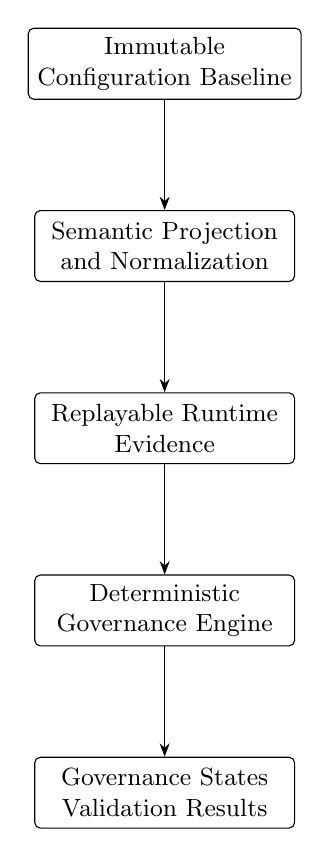
\begin{tikzpicture}[
    node distance=1.4cm,
    >=Stealth,
    box/.style={
        draw,
        rounded corners=2pt,
        align=center,
        minimum width=3.3cm,
        minimum height=0.9cm,
        font=\small
    }
]

\node[box] (baseline) {Immutable\\Configuration Baseline};

\node[box, below=of baseline] (projection) {Semantic Projection\\and Normalization};

\node[box, below=of projection] (runtime) {Replayable Runtime\\Evidence};

\node[box, below=of runtime] (engine) {Deterministic\\Governance Engine};

\node[box, below=of engine] (results) {Governance States\\Validation Results};

\draw[->] (baseline) -- (projection);
\draw[->] (projection) -- (runtime);
\draw[->] (runtime) -- (engine);
\draw[->] (engine) -- (results);

\end{tikzpicture}
    \caption{Deterministic governance pipeline supporting reproducibility and replicability. Immutable configuration baselines, semantic projection, replayable runtime evidence, and deterministic governance computation together enable independent reproduction of governance results without requiring deterministic LLM outputs.}
    \label{fig:reproducibility_pipeline}
\end{figure}

\subsection{Mitigation Strategies}
\label{sec:mitigation_strategies}

Although the preceding subsections identify several limitations affecting the present study, a number of methodological choices were deliberately adopted to reduce their impact on the reported results. Rather than attempting to maximize the breadth of the evaluation, the experimental methodology emphasizes internal consistency, deterministic governance semantics, and explicit separation between conceptual modeling, operationalization, and experimental validation.

First, the reference model was intentionally designed independently of any particular execution framework. The semantic projection architecture isolates framework-specific extraction mechanisms from the governance kernel, allowing the latter to remain unchanged across heterogeneous orchestration paradigms. This separation reduces implementation bias and facilitates the extension of the evaluation to additional frameworks without modifying the underlying governance semantics.

Second, the evaluation relies on normative governance scenarios rather than application-specific benchmarks. Each scenario targets a well-defined property of the reference model, such as lifecycle management, dependency propagation, assurance computation, baseline validation, or runtime governance. This scenario-driven methodology improves the traceability between the formal specification, the reference implementation, and the experimental evidence.

Third, reproducibility is reinforced through deterministic governance computation, immutable configuration revisions, canonical serialization, replayable runtime evidence, and automated validation procedures. These mechanisms ensure that governance outcomes depend exclusively on governed configurations and observed runtime events rather than on the stochastic behavior of the underlying language models.

In conclusion, this article deliberately distinguishes between the conceptual reference model, its formal governance semantics, the reference implementation, and the experimental evaluation. This separation avoids conflating theoretical contributions with implementation artifacts and allows future implementations to validate the same governance semantics independently of the current prototype.

Table~\ref{tab:mitigation_strategies} summarizes the principal threats identified in this section together with the corresponding mitigation strategies adopted throughout the study.

\begin{table}[t]
\caption{Summary of Threats and Mitigation Strategies}
\label{tab:mitigation_strategies}
\centering
\begin{tabular}{p{4.2cm}p{3.9cm}}
\toprule
\textbf{Threat} & \textbf{Mitigation Strategy} \\
\midrule
Limited framework coverage &
Evaluation across heterogeneous orchestration paradigms; framework-independent governance kernel. \\

Incomplete formal verification &
Executable formal semantics supported by deterministic implementation and normative validation scenarios. \\

Limited empirical generalization &
Conservative interpretation of results; explicit delimitation of the evaluation scope. \\

Implementation-dependent bias &
Separation between semantic projection, governance kernel, and framework adapters. \\

Experimental reproducibility &
Immutable revisions, replayable runtime events, canonical serialization, and automated validation suite. \\

Framework evolution &
Projection architecture designed to accommodate additional adapters without modifying the reference model. \\
\bottomrule
\end{tabular}
\end{table}

\subsection{Section Summary}
\label{sec:threats_summary}

The objective of this section has been to delimit the scope within which the conclusions of the present study should be interpreted. The identified threats do not challenge the internal consistency of the ACM reference model nor the coherence of its governance semantics. Instead, they primarily concern the breadth of the experimental validation, the current level of formal verification, and the extent to which the reported results can be generalized across the rapidly evolving landscape of agentic systems.

The experimental methodology intentionally favors methodological rigor over exhaustive coverage by combining a framework-independent governance representation, executable governance semantics, deterministic validation procedures, and reproducible experimental artifacts. Within this scope, the reported results provide credible evidence supporting the feasibility and expressiveness of the proposed governance model while avoiding claims that extend beyond the evaluated configurations.

These limitations naturally define the next stage of the research agenda. In particular, extending the empirical validation to additional orchestration paradigms, strengthening the formal verification of the governance semantics, and broadening the ecosystem supported by semantic projection represent logical continuations of the present work. These directions are discussed in the following section.

\section{Future Work}
\label{sec:future_work}

The ACM reference model introduced in this paper constitutes an initial step toward a framework-independent approach to the governance of agentic systems. The proposed metamodel, governance semantics, reference implementation, and experimental evaluation collectively demonstrate the feasibility of this approach within the scope considered in the present study. At the same time, the limitations identified in the previous section highlight several opportunities for extending both the theoretical foundations and the practical applicability of ACM.

Future research therefore naturally follows three complementary directions. The first concerns the evolution of the reference model itself to accommodate emerging abstractions while preserving its governance principles. The second focuses on strengthening the empirical and theoretical validation of the proposed semantics through broader experimental studies and formal verification. The long-term perspective is to position ACM as a common governance layer capable of interoperating with the rapidly expanding ecosystem of agentic development, deployment, and observability platforms.

\subsection{Extension of the Reference Model}
\label{sec:future_reference_model}

The reference model presented in this paper intentionally focuses on the minimal set of governance concepts required to represent heterogeneous agentic systems independently of their execution framework. This design choice favors conceptual stability and limits the number of core abstractions to those introducing distinct governance semantics. Nevertheless, the rapid evolution of agentic ecosystems will inevitably lead to the emergence of new configuration artifacts, interaction patterns, and execution abstractions that may require additional modeling capabilities.

A primary direction for future research is therefore the controlled evolution of the ACM metamodel while preserving its foundational design principles. Rather than continuously introducing framework-specific concepts into the core model, future extensions should remain guided by semantic necessity: a new abstraction should only become part of the reference model if it introduces governance properties that cannot be represented through the existing concepts and relationships. This principle preserves the framework independence of ACM while avoiding unnecessary growth of the metamodel.

An important example concerns reusable composite capabilities that are increasingly appearing under different names across modern agentic platforms, such as skills, reusable workflows, capability modules, or packaged execution components. Although these constructs differ in their implementation details, they frequently encapsulate existing governed artifacts—including prompts, tools, models, policies, workflows, and external resources—rather than introducing fundamentally new governance semantics. Consequently, many of these emerging abstractions can already be represented through semantic projection as governed composite configuration items without requiring modifications to the ACM core.

An additional extension concerns Retrieval-Augmented Generation (RAG) systems, which are becoming a fundamental building block of modern agentic applications. Rather than introducing a dedicated governance abstraction, ACM can represent RAG pipelines through the composition of existing configuration items, including embedding models, retrieval policies, vector indexes, knowledge repositories, prompt definitions, and retrieval components. This representation enables immutable versioning of the complete retrieval configuration, explicit provenance of derived vector indexes, and governance of retrieval policies independently of the underlying storage technology. Consequently, ACM can govern the evolution of retrieval-augmented systems without embedding retrieval-specific concepts into its core metamodel.

Another important direction concerns self-learning or continuously adaptive agents. Such systems challenge traditional configuration management because parts of their operational behavior may evolve autonomously through accumulated experience, parameter adaptation, or long-term memory updates. Extending ACM to distinguish immutable governed configurations from controlled runtime knowledge evolution would enable adaptive systems to remain auditable while preserving reproducibility of approved configurations. Future work should therefore investigate governance semantics capable of representing learning artifacts, adaptation boundaries, and evidence associated with autonomous configuration evolution.

Finally, the increasing adoption of interoperability protocols and workflow orchestration platforms, including Model Context Protocol (MCP), Agent-to-Agent (A2A) communication, and low-code orchestration environments such as n8n, provides another opportunity for extending the reference model. Rather than incorporating protocol-specific abstractions, ACM can represent these ecosystems through semantic projection of communication endpoints, external services, orchestration workflows, and interaction contracts into governed configuration items. This approach preserves the framework-independent nature of the reference model while enabling configuration governance across heterogeneous execution environments and emerging interoperability standards.

Future extensions may also address governance capabilities that extend beyond the scope of the current reference model. Examples include distributed governance across multiple organizations, federated configuration repositories, cross-system dependency management, richer policy composition mechanisms, and governance of long-lived autonomous ecosystems whose configuration evolves continuously over time. These extensions would broaden the applicability of ACM while preserving the separation between configuration governance and execution that constitutes one of its central architectural principles.

Ultimately, the long-term evolution of ACM should prioritize conceptual stability over feature accumulation. As with mature reference models in software engineering, the objective is not to mirror every innovation introduced by individual frameworks, but rather to identify the stable governance abstractions that remain applicable despite the continuous evolution of execution technologies. This philosophy enables the reference model to evolve incrementally while maintaining interoperability, explainability, and long-term sustainability.

\subsection{Broader Framework Validation}
\label{sec:future_framework_validation}

The empirical evaluation presented in this paper intentionally focuses on two representative orchestration paradigms in order to demonstrate the feasibility of framework-independent configuration governance. Although the successful semantic projection of LangGraph and CrewAI provides encouraging evidence supporting the proposed reference model, broader validation across the rapidly evolving landscape of agentic systems remains an essential research direction.

Future work should therefore extend the experimental corpus to additional execution frameworks exhibiting different orchestration principles and configuration abstractions. In particular, frameworks supporting dynamic handoffs, hierarchical delegation, event-driven coordination, decentralized multi-agent collaboration, or long-running autonomous workflows would provide valuable opportunities to evaluate the expressiveness of the ACM metamodel under substantially different execution models.

Beyond execution frameworks themselves, validation could also incorporate complementary components of the emerging AgentOps and LLMOps ecosystem. Provenance platforms, observability infrastructures, evaluation frameworks, and deployment management systems increasingly expose governance-relevant metadata that could naturally participate in semantic projection. Studying the integration of ACM with such platforms would provide additional evidence regarding the ability of the reference model to serve as a common governance layer across heterogeneous operational environments.

Another important direction concerns empirical validation at industrial scale. The current experiments intentionally emphasize semantic correctness rather than operational scalability. Future studies should therefore evaluate ACM on large agentic systems involving hundreds or thousands of governed configuration items, long-lived execution histories, continuously evolving baselines, and collaborative governance processes distributed across multiple development teams. Such evaluations would provide quantitative evidence regarding scalability, governance overhead, and operational usability in realistic production environments.

Ultimately, extending the experimental validation is not intended merely to increase the number of supported frameworks. Rather, it aims to progressively strengthen the empirical evidence supporting the central hypothesis of this work: that governance semantics can remain stable despite the continuous evolution of agentic execution technologies.

\subsection{Formal Verification of Governance Semantics}
\label{sec:future_formal_verification}

The governance semantics introduced in this paper are defined through a formal operational specification and validated through deterministic execution of the reference implementation. While this approach demonstrates the practical executability of the proposed semantics, it does not constitute a formal mathematical proof of their correctness. Establishing such guarantees represents an important direction for future research.

One immediate objective concerns the verification of the fixed-point propagation algorithm underlying governance state computation. Formal proofs could establish properties such as termination, determinism, convergence toward a unique governance state, and independence from evaluation order. Demonstrating these properties would strengthen confidence that governance decisions remain stable regardless of implementation details or execution strategies.

A second research direction involves the formal analysis of the lifecycle semantics themselves. The lifecycle state machines, dependency propagation rules, assurance composition mechanisms, and runtime governance semantics could be expressed within a formal verification framework in order to prove invariants such as transition consistency, absence of contradictory governance states, preservation of dependency constraints, and correctness of state propagation under arbitrary configuration topologies.

Beyond individual algorithms, future work may investigate the formal specification of the ACM reference model as a complete governance system. Model-checking techniques, temporal logic, theorem proving, or specification languages dedicated to distributed systems could be employed to verify global properties of the governance semantics and to detect inconsistencies automatically during the evolution of the reference model. Such approaches would complement the current implementation-based validation with machine-verifiable correctness guarantees.

Formal verification would facilitate the development of independent ACM implementations. By providing mathematically specified governance semantics rather than relying solely on behavioral equivalence with the reference implementation, future implementations could demonstrate conformance through proof of semantic equivalence instead of implementation similarity. This evolution would represent an important step toward establishing ACM as a stable and implementation-independent governance specification.

\subsection{Toward an Agentic Configuration Ecosystem}
\label{sec:future_ecosystem}

The rapid maturation of agentic software engineering has led to the emergence of a rich ecosystem of complementary technologies dedicated to development, deployment, observability, evaluation, provenance, and operational governance. Rather than replacing these existing tools, ACM is intended to provide a framework-independent governance layer capable of connecting heterogeneous components through a common semantic representation of governed configuration artifacts.

A promising direction for future research therefore consists in studying the integration of ACM with broader AgentOps and LLMOps ecosystems. Modern observability platforms increasingly collect execution traces, evaluation results, model usage metrics, cost information, and provenance metadata that constitute valuable inputs for governance processes. Conversely, governance decisions produced by ACM could enrich these platforms with lifecycle status, assurance levels, configuration lineage, dependency analysis, and compliance information, providing a higher semantic level for operational monitoring.

Another important perspective concerns the integration of ACM with software engineering infrastructures. Continuous integration and deployment pipelines, software configuration management systems, artifact repositories, and supply-chain security mechanisms already manage the lifecycle of conventional software assets. Extending these infrastructures to incorporate governed agentic configuration items would enable unified governance across both traditional software components and AI-native artifacts while preserving traceability throughout the complete development lifecycle.

Beyond tooling integration, future work may explore the definition of interoperable governance services exposing standardized interfaces for semantic projection, configuration validation, governance state computation, and provenance exchange. Such services would facilitate the development of heterogeneous toolchains in which execution frameworks, observability platforms, deployment systems, and governance engines cooperate while remaining independently evolvable.

Ultimately, the long-term objective is to establish ACM not as another execution platform, but as a common semantic governance layer capable of interconnecting the diverse technologies that increasingly compose modern agentic software ecosystems.

\subsection{Standardization Perspectives}
\label{sec:future_standardization}

The absence of a common vocabulary and shared governance abstractions currently represents one of the principal obstacles to interoperability across agentic systems. While execution frameworks continue to evolve rapidly, equivalent concepts are frequently described using framework-specific terminology, making configuration exchange, governance portability, and comparative evaluation unnecessarily difficult.

The ACM reference model represents an initial step toward addressing this fragmentation by proposing a framework-independent conceptual vocabulary together with formally defined governance semantics. Although the present work does not aim to establish a standard, it provides a structured foundation upon which future community discussions regarding interoperable governance models may build.

Future research may therefore investigate the definition of standardized exchange formats for governed configuration items, semantic projection interfaces, governance evidence, provenance information, and lifecycle metadata. Such specifications would facilitate interoperability between heterogeneous execution frameworks while allowing governance information to remain portable independently of implementation technologies. Likewise, standardized conformance criteria could enable independent implementations to demonstrate semantic compatibility with the ACM reference model while preserving implementation freedom.

The maturation of ACM may also benefit from collaboration with broader software engineering and artificial intelligence communities working on software configuration management, software supply-chain security, provenance, and AI governance. Aligning ACM with existing standards whenever appropriate would facilitate its integration into established engineering practices while reducing duplication of concepts that are already well understood in adjacent disciplines.

Ultimately, the long-term ambition is not to standardize a particular implementation, but to encourage convergence toward a shared governance language for agentic systems towards an agentic configuration ecosystem. By separating governance semantics from execution technologies, ACM provides a stable conceptual foundation that could evolve collaboratively as the agentic landscape continues to mature. Such convergence would improve interoperability, reproducibility, auditability, and long-term sustainability across heterogeneous agentic platforms. Such anglobal agentic ecosystem, including ACM, could progressively evolve toward interoperable configuration exchange and, ultimately, contribute to future standardization efforts for governed agentic systems.

\section{Conclusion}
\label{sec:conclusion}

The rapid evolution of agentic software engineering has fundamentally transformed the role of configuration artifacts. Prompts, tools, execution graphs, policies, models, runtime state, and provenance have become first-class engineering assets whose governance can no longer rely solely on traditional software configuration management practices. At the same time, the increasing diversity of orchestration frameworks has introduced heterogeneous configuration abstractions, making governance difficult to reproduce, audit, and compare across platforms.

This paper introduced Agentic Configuration Management (ACM), a framework-independent governance representation for the governance of agentic systems. Rather than proposing another execution framework, ACM separates governance semantics from execution technologies through a unified representation of governed configuration items, immutable revisions, semantic relationships, deterministic lifecycle management, assurance semantics, and runtime governance. This separation enables heterogeneous agentic systems to be represented within a common governance model while preserving the flexibility of existing orchestration frameworks.

Beyond the conceptual contribution, the paper demonstrated that the proposed semantics can be operationalized through a reference implementation and evaluated using representative orchestration paradigms. The experimental results show that heterogeneous agentic configurations can be semantically projected into a common governance representation while preserving the information required for deterministic governance decisions. Although the current evaluation remains intentionally limited in scope, it provides initial empirical evidence supporting the feasibility of framework-independent configuration governance for agentic systems.

More broadly, this work argues that governance should become an explicit architectural layer of agentic software engineering rather than an implementation-specific concern embedded within individual execution frameworks. By introducing a common vocabulary, formally defined governance semantics, and a framework-independent governance representation, ACM establishes a foundation upon which future research can investigate interoperability, formal verification, scalable governance, and standardized configuration management practices for increasingly autonomous AI systems.

Ultimately, the contribution of ACM is not to prescribe how agentic systems should execute, but to provide a stable semantic foundation for governing how they are specified, versioned, validated, traced, and evolved. As agentic ecosystems continue to diversify, such a separation between execution and governance may become an essential prerequisite for building reproducible, auditable, interoperable, and trustworthy AI systems.

%%%%%%%%%%%%%%%%%%%%%%%%%%%%%%%%%%%%%%%%%%%%%%%%%%%%%%%%%%%%%%%%%%%%%%%%%%%%%%%%
\appendices

\section{Related Work}
\label{appendix:related_work}
\subsubsection{Framework Comparison}
Table~\ref{tab:framework_comparison} summarizes representative characteristics of several widely used agentic frameworks.
\begin{table*}[t]
	\centering
	\caption{Representative characteristics of widely used agentic frameworks. The comparison illustrates the diversity of execution paradigms while highlighting the absence of a common configuration representation.}
	\label{tab:framework_comparison}
	
	\renewcommand{\arraystretch}{1.15}
	
	\begin{tabular}{p{3.2cm}p{3.1cm}p{3.4cm}p{3.4cm}c}
		\toprule
		\textbf{Framework}
		&
		\textbf{Primary Paradigm}
		&
		\textbf{Execution Model}
		&
		\textbf{Native Configuration Abstraction}
		\\
		\midrule
		
		LangGraph
		&
		State graph
		&
		Explicit graph execution
		&
		Nodes, edges and shared state
		\\
		
		CrewAI
		&
		Role-based multi-agent
		&
		Agents, tasks and crews
		&
		Agents, tasks, crews and flows
		\\
		
		OpenAI Agents SDK
		&
		Delegation-based agents
		&
		Handoffs and tool orchestration
		&
		Agents, tools and handoffs
		\\
		
		Microsoft Agent Framework
		&
		Workflow orchestration
		&
		Agent workflows
		&
		Workflow definitions
		\\
		
		Google ADK
		&
		Hierarchical agents
		&
		Multi-agent orchestration
		&
		Agent hierarchies
		\\
		
		\bottomrule
	\end{tabular}
	
\end{table*}
\subsection{Gap Analysis}
The Table ~\ref{tab:gap_analysis_detailed} supports a comparative gap analysis between the different governance aproaches.
\begin{table*}[t]
	\centering
	\caption{Detailed rationale supporting the comparative gap analysis
		presented in Table~\ref{tab:gap_analysis}.}
	\label{tab:gap_analysis_detailed}
	
	\footnotesize
	\setlength{\tabcolsep}{3pt}
	\renewcommand{\arraystretch}{1.18}
	
	\begin{tabularx}{\textwidth}{
			>{\RaggedRight\arraybackslash}p{3.25cm}
			C{1.05cm}
			C{1.15cm}
			C{1.45cm}
			C{1.30cm}
			C{0.85cm}
			Y
		}
		\toprule
		
		\textbf{Governance capability}
		&
		\makecell{\textbf{SCM}}
		&
		\makecell{\textbf{AI}\\\textbf{Gov.}}
		&
		\makecell{\textbf{LLMOps /}\\\textbf{AgentOps}}
		&
		\makecell{\textbf{Agent}\\\textbf{frameworks}}
		&
		\makecell{\textbf{ACM}}
		&
		\textbf{Rationale}
		\\
		
		\midrule
		
		Configuration identification
		&
		$\checkmark$
		&
		$\sim$
		&
		$\sim$
		&
		$\sim$
		&
		$\checkmark$
		&
		SCM explicitly identifies configuration items.
		Other approaches identify only the artefacts relevant to their
		respective governance, operational, or execution objectives.
		ACM represents heterogeneous artefacts as governed ACI revisions.
		\\
		
		Version management
		&
		$\checkmark$
		&
		--
		&
		$\sim$
		&
		$\sim$
		&
		$\checkmark$
		&
		SCM provides mature version control.
		LLMOps platforms and agent frameworks version selected artefacts,
		such as prompts or workflows, but not complete governed
		configurations.
		ACM assigns immutable revisions to every governed artefact.
		\\
		
		Configuration provenance
		&
		$\sim$
		&
		$\checkmark$
		&
		$\checkmark$
		&
		$\sim$
		&
		$\checkmark$
		&
		SCM preserves software history, while AI governance and LLMOps
		emphasize provenance, accountability, and traceability.
		Frameworks expose partial execution provenance.
		ACM links configuration, revision, runtime, and evidence provenance.
		\\
		
		Dependency traceability
		&
		$\checkmark$
		&
		$\sim$
		&
		$\checkmark$
		&
		$\sim$
		&
		$\checkmark$
		&
		SCM manages software dependencies, and LLMOps relates selected
		artefacts such as prompts, traces, and evaluations.
		Frameworks expose dependencies through native abstractions.
		ACM explicitly models typed dependencies across heterogeneous
		configuration artefacts.
		\\
		
		Execution observability
		&
		--
		&
		$\sim$
		&
		$\checkmark$
		&
		$\checkmark$
		&
		$\checkmark$
		&
		Execution monitoring is not a primary SCM capability.
		AI governance recommends monitoring, whereas LLMOps platforms and
		agent frameworks provide traces and runtime telemetry.
		ACM incorporates normalized runtime observations into its governance
		representation.
		\\
		
		Lifecycle governance
		&
		$\sim$
		&
		$\checkmark$
		&
		$\sim$
		&
		$\sim$
		&
		$\checkmark$
		&
		SCM governs controlled software evolution, and AI governance defines
		processes across the AI lifecycle.
		Operational platforms and frameworks mainly address deployment or
		execution stages.
		ACM governs the lifecycle of exact configuration revisions.
		\\
		
		Framework-independent representation
		&
		--
		&
		--
		&
		--
		&
		--
		&
		$\checkmark$
		&
		Existing approaches remain centred on software artefacts,
		organizational processes, operational platforms, or native execution
		models.
		ACM provides a framework-independent representation of governed
		agentic configurations.
		\\
		
		Unified configuration model
		&
		--
		&
		--
		&
		--
		&
		--
		&
		$\checkmark$
		&
		No other family combines heterogeneous artefacts, immutable
		revisions, typed dependencies, governance semantics, and runtime
		traceability within one reference model.
		This integration constitutes ACM's primary contribution.
		\\
		
		\bottomrule
	\end{tabularx}
	
	\vspace{0.4em}
	
	{\scriptsize
		$\checkmark$ Fully addressed
		\hspace{1em}
		$\sim$ Partially addressed
		\hspace{1em}
		-- Not provided as a primary capability.
	}
	
\end{table*}
	

\section{Formal Foundations}
\label{appendix:formal_foundations}

This appendix provides the mathematical definitions supporting the governance semantics introduced in Section~\ref{sec:governance_semantics}. It complements the normative presentation without introducing additional governance concepts.

\subsection{Configuration Graph}

The ACM reference model is defined over a finite directed graph

\begin{equation}
	G=(V,E),
	\label{eq:graph_definition}
\end{equation}

where:

\begin{itemize}
	\item $V$ denotes the finite set of immutable ACI revisions;
	\item $E\subseteq V\times V\times T_R$ denotes the finite set of typed governance relationships;
	\item $T_R$ is the finite set of relationship types defined by the reference metamodel.
\end{itemize}

The graph topology remains immutable for a given revision set. Configuration evolution is represented by introducing new immutable revisions rather than modifying existing vertices.

\subsection{Governance Descriptor}

Each revision $v\in V$ is associated with a governance descriptor

\begin{equation}
	\Gamma(v)=
	\left(
	L(v),
	Q(v),
	A(v),
	I(v),
	El(v),
	Rt(v)
	\right),
	\label{eq:descriptor_definition}
\end{equation}

where every component belongs to an independent governance state space.

The governance descriptor represents the complete governance status of an ACI revision at a given observation point. It serves exclusively as a logical aggregation of the different semantic dimensions and introduces no computational semantics.

All semantic computations are defined through dedicated evaluation functions introduced later in this appendix.

\subsection{Notation}

Throughout the remainder of this appendix, lowercase functions denote state assignments associated with a revision:

\begin{equation}
	X:V\rightarrow\mathcal{X},
	\label{eq:state_assignment}
\end{equation}

where $\mathcal{X}$ denotes the corresponding governance state space.

This convention is uniformly applied to lifecycle, quality, assurance, impact, eligibility, and runtime semantics.

For propagation reasoning, an impact valuation is a state assignment

\begin{equation}
	\iota : V \rightarrow \mathcal{I},
	\label{eq:impact_valuation}
\end{equation}

where $\iota(v)$ denotes the propagated impact state associated with revision
$v$. For a fixed configuration graph, the set of all impact valuations is

\begin{equation}
	\mathcal{D}_{G}
	=
	\mathcal{I}^{V}.
	\label{eq:impact_valuation_domain}
\end{equation}

The graph structure and the propagation-policy mapping remain fixed during one
propagation computation. Only the impact valuation evolves.

\section{Governance State Spaces}
\label{appendix:state_spaces}

This appendix formally defines the governance state spaces introduced in Section~\ref{sec:governance_state_spaces}. Each state space represents an independent semantic dimension.

\subsection{Lifecycle}

The lifecycle state space is defined as

\begin{equation}
	\mathcal{L}=
	\{
	Draft,
	Validated,
	Approved,
	Released,
	Deprecated,
	Archived
	\}.
	\label{eq:lifecycle_space}
\end{equation}

The ordering relation is the monotonic lifecycle order introduced in Equation~(\ref{eq:lifecycle_order}).

---

\subsection{Quality}

The quality state space is defined as

\begin{equation}
	\mathcal{Q}=
	\{
	Undefined,
	Valid,
	Warning,
	Invalid
	\}.
	\label{eq:quality_space}
\end{equation}

The quality state reflects the intrinsic validation status of an individual revision independently of its dependencies.

---

\subsection{Assurance}

The assurance state space is defined as

\begin{equation}
	\mathcal{A}=
	\{
	Unassessed,
	Partial,
	Satisfied
	\}.
	\label{eq:assurance_space}
\end{equation}

The assurance state represents the availability of governance evidence associated with a revision.

The corresponding ordering relation is

\begin{equation}
	Unassessed
	<
	Partial
	<
	Satisfied.
	\label{eq:assurance_order}
\end{equation}

---

\subsection{Impact}

The impact state space is defined as

\begin{equation}
	\mathcal{I}=
	\{
	None,
	Local,
	Propagated
	\}.
	\label{eq:impact_space}
\end{equation}

The impact space is equipped with the total order

\begin{equation}
	None
	\prec_{\mathcal I}
	Local
	\prec_{\mathcal I}
	Propagated.
	\label{eq:impact_order}
\end{equation}

Its least element is

\begin{equation}
	\bot_{\mathcal{I}}
	=
	None.
	\label{eq:impact_bottom}
\end{equation}

The least upper bound of two impact states is defined by

\begin{equation}
	i_1
	\sqcup_{\mathcal{I}}
	i_2
	=
	\max\nolimits_{\prec_{\mathcal{I}}}
	\left(i_1,i_2\right).
	\label{eq:impact_join}
\end{equation}

Consequently,
$\left(\mathcal{I},\preceq_{\mathcal{I}}\right)$ is a finite lattice.

The impact state identifies whether a revision has been affected by a propagated governance change.
---

\subsection{Eligibility}

The eligibility state space is defined as

\begin{equation}
	\mathcal{E}=
	\{
	Blocked,
	Restricted,
	Eligible
	\}.
	\label{eq:eligibility_space}
\end{equation}

The corresponding ordering relation is

\begin{equation}
	Blocked
	<
	Restricted
	<
	Eligible.
	\label{eq:eligibility_order}
\end{equation}

The eligibility state summarizes whether a revision satisfies the governance conditions required for operational use.

---

\subsection{Runtime}

The runtime state space is defined as

\begin{equation}
	\mathcal{R}=
	\{
	Created,
	Ready,
	Running,
	Waiting,
	Completed,
	Failed,
	Cancelled,
	Terminated
	\}.
	\label{eq:runtime_space}
\end{equation}

The runtime state represents the execution status reconstructed from runtime observations independently of the configuration lifecycle.

Unlike the previous state spaces, runtime states are reconstructed from execution events rather than assigned through governance decisions.



\section{Propagation Policies}
\label{appendix:propagation_policies}

This appendix formally defines the propagation policies introduced in Section~\ref{sec:propagation_policies}. Propagation policies characterize how governance information traverses configuration relationships independently of the governance state evaluation.

\subsection{Policy Space}

Let $T_R$ denote the finite set of relationship types defined by the ACM reference model.

Each relationship type is associated with exactly one propagation policy through the mapping

\begin{equation}
	\Pi : T_R \rightarrow \mathcal{P},
	\label{eq:policy_function}
\end{equation}

where the policy space is defined as

\begin{equation}
	\mathcal{P}=
	\left\{
	\textit{Blocking},
	\textit{Warning},
	\textit{Informational},
	\textit{None}
	\right\}.
	\label{eq:policy_set}
\end{equation}

The mapping $\Pi$ is static and depends only on the relationship type. Consequently, identical relationship types always induce identical propagation behavior independently of the connected revisions.

\subsection{Policy Precedence}

When several propagation paths converge on the same revision, multiple propagation policies may simultaneously apply. Their effective behavior is determined by a total precedence relation over $\mathcal{P}$.

The precedence relation is defined as

\begin{equation}
	\textit{Blocking}
	>
	\textit{Warning}
	>
	\textit{Informational}
	>
	\textit{None}.
	\label{eq:policy_order}
\end{equation}

This ordering reflects increasing governance severity and guarantees deterministic propagation independently of graph traversal order.

\subsection{Policy Composition}

The effective propagation policy associated with a revision receiving multiple propagated events is obtained by selecting the highest-precedence policy.

The composition operator

\begin{equation}
	\otimes :
	\mathcal{P}\times\mathcal{P}
	\rightarrow
	\mathcal{P},
	\label{eq:policy_composition}
\end{equation}

is therefore defined as

\begin{equation}
	p_1\otimes p_2
	=
	\max\nolimits_{(\ref{eq:policy_order})}
	\left(p_1,p_2\right),
	\label{eq:policy_max}
\end{equation}

where the maximum is evaluated according to the precedence relation defined in Equation~(\ref{eq:policy_order}).

By construction, the composition operator satisfies

\begin{itemize}
	\item commutativity,
	\item associativity,
	\item idempotence.
\end{itemize}

Consequently, policy composition is independent of propagation order, parent ordering, and graph traversal strategy.

These properties ensure that the propagation operator introduced in Appendix~\ref{appendix:propagation_semantics} produces deterministic governance results.

Policy precedence determines how concurrent policy contributions are combined.
The effect of an individual policy on an impact state is specified separately
by the local transfer semantics introduced in
Appendix~\ref{appendix:propagation_semantics}. Policy composition and impact
transfer therefore remain distinct operations: the former selects the effective
policy, whereas the latter determines its contribution to impact propagation.

\section{Formal Evaluation Functions}
\label{appendix:evaluation_functions}

This appendix formally defines the governance evaluation functions introduced in Section~\ref{sec:evaluation_functions}. These functions assign governance states independently of propagation semantics.

\subsection{Quality Evaluation}

The quality evaluation function

\begin{equation}
	f_{\mathrm{quality}} : V \rightarrow \mathcal{Q},
	\label{eq:quality_function}
\end{equation}

assigns exactly one quality state to every ACI revision.

Consequently,

\begin{equation}
	\forall v\in V,\;
	\exists!\;
	Q(v)\in\mathcal{Q}.
	\label{eq:quality_total}
\end{equation}

\subsection{Assurance Evaluation}

Similarly,

\begin{equation}
	f_{\mathrm{assurance}} : V \rightarrow \mathcal{A},
	\label{eq:assurance_function}
\end{equation}

assigns a unique assurance state to every revision.

Therefore,

\begin{equation}
	\forall v\in V,\;
	\exists!\;
	A(v)\in\mathcal{A}.
	\label{eq:assurance_total}
\end{equation}

\subsection{Eligibility Evaluation}

Eligibility is evaluated locally from the lifecycle, quality, assurance, and
stabilized impact states associated with a revision. Propagation policies do
not constitute an argument of the eligibility function; their effects are
already reflected in the propagated impact state.

Formally,

\begin{equation}
	f_{\mathrm{elig}} :
	\mathcal{L}
	\times
	\mathcal{Q}
	\times
	\mathcal{A}
	\times
	\mathcal{I}
	\rightarrow
	\mathcal{E}.
	\label{eq:eligibility_function}
\end{equation}

The function is deterministic.

\begin{equation}
	\forall
	(l,q,a,i)
	\in
	\mathcal{L}
	\times
	\mathcal{Q}
	\times
	\mathcal{A}
	\times
	\mathcal{I},
	\;
	\exists!\;
	e
	\in
	\mathcal{E}
	\text{ such that }
	e
	=
	f_{\mathrm{elig}}(l,q,a,i).
	\label{eq:eligibility_deterministic}
\end{equation}
For each revision $v\in V$, eligibility is therefore obtained from the final
impact valuation $\iota^{*}$ computed by the propagation semantics:

\begin{equation}
	El(v)
	=
	f_{\mathrm{elig}}
	\left(
	L(v),
	Q(v),
	A(v),
	\iota^{*}(v)
	\right).
	\label{eq:eligibility_from_fixed_impact}
\end{equation}

Eligibility evaluation is not part of the fixed-point iteration and does not
modify the propagated impact valuation.

The evaluation functions are defined as total deterministic mappings over their
respective finite domains. They introduce no dependency traversal and do not
modify the configuration graph. In particular, eligibility evaluation consumes
the stabilized impact valuation produced by propagation but does not participate
in the propagation fixed-point computation.

%%%%%%%%%%%%%%%%%%%%%%%%%%%%%%%%%%%%%%%%%%%%%%%%%%%%%%%%%%%%%%%%%%%%%%%%%%%%%%%%
\section{Propagation Semantics}
\label{appendix:propagation_semantics}

This appendix formalizes the propagation semantics introduced in
Section~\ref{subsec:propagation_semantics}. It specifies the propagation
operator, the fixed-point semantics, and the reference worklist algorithm.
The mathematical properties of the propagation semantics, including monotonicity,
termination, convergence, and correctness, are established separately in
Appendix ~\ref{appendix:formal_properties}.

%%%%%%%%%%%%%%%%%%%%%%%%%%%%%%%%%%%%%%%%%%%%%%%%%%%%%%%%%%%%%%%%%%%%%%%%%%%%%%%%
\subsection{Propagation Operator}

Propagation operates over a fixed governed configuration graph

\[
G=(V,E),
\]

whose structure remains unchanged throughout one propagation computation.
Only propagated impact states evolve during the evaluation.

As introduced in Appendix~\ref{appendix:formal_foundations}, an impact valuation
is a mapping

\[
\iota : V \rightarrow \mathcal{I},
\]

where $\iota(v)$ denotes the current propagated impact state associated with
revision $v$.

The propagation process starts from an initial valuation

\begin{equation}
	\iota^{(0)} : V \rightarrow \mathcal{I},
	\label{eq:initial_impact_valuation}
\end{equation}

which identifies the revisions directly affected by the governance event.
Revisions not affected by the initial event are assigned the least impact state

\[
\bot_{\mathcal I}=None.
\]

The graph structure and the propagation-policy mapping remain fixed throughout
the computation. Consequently, propagation modifies only the impact valuation.

%%%%%%%%%%%%%%%%%%%%%%%%%%%%%%%%%%%%%%%%%%%%%%%%%%%%%%%%%%%%%%%%%%%%%%%%%%%%%%%%

Each relationship

\[
e=(u,v)\in E
\]

is associated with a propagation policy

\[
\Pi(e)\in\mathcal P,
\]

defined in Appendix~\ref{appendix:propagation_policies}.

For formal reasoning, each propagation policy induces a local transfer function

\begin{equation}
	\tau_p :
	\mathcal I
	\rightarrow
	\mathcal I,
	\qquad
	p\in\mathcal P,
	\label{eq:transfer_function}
\end{equation}

which specifies how the propagated impact state is transmitted across a single
relationship governed by policy $p$.

The precise behavior of each transfer function is determined by the associated
propagation policy while preserving the ordering relation defined on
$\mathcal I$.

%%%%%%%%%%%%%%%%%%%%%%%%%%%%%%%%%%%%%%%%%%%%%%%%%%%%%%%%%%%%%%%%%%%%%%%%%%%%%%%%

For every revision $v\in V$, propagation is defined by the local evaluation
function

\begin{equation}
	\label{eq:local_transfer}
	F_v(\iota)
	=
	\iota^{(0)}(v)
	\sqcup_{\mathcal I}
	\bigvee_{(u,v)\in E}
	\tau_{\Pi(u,v)}
	\!\left(
	\iota(u)
	\right),
\end{equation}

where $\sqcup_{\mathcal I}$ denotes the least upper bound on the impact lattice.

For a revision with no incoming relationship, the empty join is defined as the
least impact state:

\begin{equation}
	\bigvee_{\varnothing}
	=
	\bot_{\mathcal I}.
	\label{eq:empty_impact_join}
\end{equation}

The first term preserves the initial impact directly associated with the
governance event, whereas the second term aggregates the propagated
contributions received from predecessor revisions.

%%%%%%%%%%%%%%%%%%%%%%%%%%%%%%%%%%%%%%%%%%%%%%%%%%%%%%%%%%%%%%%%%%%%%%%%%%%%%%%%

The global propagation operator is therefore defined as

\begin{equation}
	\label{eq:impact_operator}
	\widehat{\mathrm{Prop}}_{G,\Pi}
	:
	\mathcal D_G
	\rightarrow
	\mathcal D_G,
\end{equation}

with

\begin{equation}
	\label{eq:impact_operator_definition}
	\widehat{\mathrm{Prop}}_{G,\Pi}(\iota)(v)
	=
	F_v(\iota),
	\qquad
	\forall v\in V.
\end{equation}

The operator acts exclusively on impact valuations.
Lifecycle, quality, assurance, and eligibility states are not modified during
propagation. Once the impact valuation has stabilized, eligibility is evaluated
locally using the function
$f_{\mathrm{elig}}$
defined in Appendix~\ref{appendix:evaluation_functions}.

For readability, the remainder of this appendix denotes
$\widehat{\mathrm{Prop}}_{G,\Pi}$ simply by
$\widehat{\mathrm{Prop}}$
whenever the underlying graph and propagation-policy mapping are fixed.

%%%%%%%%%%%%%%%%%%%%%%%%%%%%%%%%%%%%%%%%%%%%%%%%%%%%%%%%%%%%%%%%%%%%%%%%%%%%%%%%
\subsection{Least Fixed-Point Semantics}

Starting from the initial impact valuation
$\iota^{(0)}$, successive applications of the propagation operator generate the
sequence

\begin{equation}
	\label{eq:impact_iteration}
	\iota^{(k+1)}
	=
	\widehat{\mathrm{Prop}}
	\!\left(
	\iota^{(k)}
	\right),
\end{equation}

where $k$ denotes the propagation iteration.

Propagation continues until the impact valuation becomes stable, that is, until
an additional application of the propagation operator produces no further
modification.

The stabilized valuation therefore satisfies

\begin{equation}
	\label{eq:impact_fixed_point}
	\iota^{*}
	=
	\widehat{\mathrm{Prop}}
	\!\left(
	\iota^{*}
	\right).
\end{equation}

The valuation $\iota^{*}$ represents the final propagated impact state
associated with every revision of the configuration graph.

Once the impact valuation has stabilized, eligibility is evaluated
independently for every revision using the local evaluation function defined in
Appendix~\ref{appendix:evaluation_functions}. Formally,

\begin{equation}
	\label{eq:eligibility_after_propagation}
	El(v)
	=
	f_{\mathrm{elig}}
	\!\left(
	L(v),
	Q(v),
	A(v),
	\iota^{*}(v)
	\right),
	\qquad
	\forall v\in V.
\end{equation}

Consequently, the propagation phase computes only the propagated impact
valuation, whereas eligibility evaluation is performed afterwards as an
independent local computation. This separation eliminates any circular
dependency between propagation and eligibility evaluation while preserving the
normative semantics introduced in Section~\ref{subsec:propagation_semantics}.

The existence, uniqueness, and convergence properties of the stabilized impact
valuation, together with the mathematical justification of the fixed-point
construction, are established in Appendix ~\ref{appendix:formal_properties}.

%%%%%%%%%%%%%%%%%%%%%%%%%%%%%%%%%%%%%%%%%%%%%%%%%%%%%%%%%%%%%%%%%%%%%%%%%%%%%%%%
\subsection{Reference Worklist Algorithm}
\label{appendix:ref_worklist_algo}
The propagation semantics specify the stable impact valuation independently of
the evaluation strategy used to compute it. Any implementation producing the
fixed point defined by Equation~(\ref{eq:impact_fixed_point}) is therefore
compliant with the reference semantics.

The reference implementation adopts a worklist-based evaluation strategy that
incrementally updates only the revisions whose propagated impact state may
change.

Initially, the current valuation is set to the initial impact valuation

\[
\iota
=
\iota^{(0)},
\]

and the worklist

\[
W
\subseteq
V
\]

contains every revision directly affected by the triggering governance event,
together with their immediate successors.

At each iteration, one revision

\[
v\in W
\]

is removed from the worklist and its local propagation equation
(Equation~(\ref{eq:local_transfer})) is evaluated using the current impact
valuation.

If the evaluation produces a strictly greater impact state,

\begin{equation}
	\label{eq:worklist_update}
	F_v(\iota)
	\succ_{\mathcal I}
	\iota(v),
\end{equation}

the valuation is updated according to

\begin{equation}
	\label{eq:worklist_assignment}
	\iota(v)
	:=
	F_v(\iota),
\end{equation}

and every successor

\[
w
\quad
\text{such that}
\quad
(v,w)\in E
\]

is inserted into the worklist if not already present.

Otherwise, no successor is scheduled and propagation continues with the next
revision contained in the worklist.

The evaluation terminates when the worklist becomes empty,

\begin{equation}
	\label{eq:worklist_stop}
	W
	=
	\varnothing.
\end{equation}

The algorithm terminates operationally when the worklist becomes empty:

\begin{equation}
	W
	=
	\varnothing.
	\label{eq:worklist_stop}
\end{equation}

Under the worklist initialization, successor rescheduling, bottom-preserving
transfer semantics, and fairness conditions defined above, an empty worklist
corresponds to a valuation satisfying every local propagation equation. The
formal implication

\begin{equation}
	W
	=
	\varnothing
	\Longrightarrow
	\forall v\in V,\;
	F_v(\iota)
	=
	\iota(v)
	\label{eq:worklist_local_equilibrium}
\end{equation}

and the equality of the resulting valuation with $\iota^{*}$ are established
in Appendix~A.6.

The reference worklist algorithm assumes a fair evaluation strategy, meaning
that every revision inserted into the worklist is eventually processed.
Different scheduling strategies, including FIFO, LIFO, or priority-based
queues, remain compliant provided that they satisfy this fairness condition and
compute the same stabilized valuation.

The correctness, termination, convergence, and complexity of the reference
worklist algorithm are established in Appendix ~\ref{appendix:formal_properties}.

%%%%%%%%%%%%%%%%%%%%%%%%%%%%%%%%%%%%%%%%%%%%%%%%%%%%%%%%%%%%%%%%%%%%%%%%%%%%%%%%
\section{Formal Properties of the Propagation Semantics}
\label{appendix:formal_properties}

This appendix establishes the mathematical properties of the propagation
semantics introduced in Appendix~\ref{appendix:propagation_semantics}. It
proves the correctness of the propagation operator, the existence and
uniqueness of the least fixed point, the convergence of the iterative
evaluation, and the correctness of the reference worklist algorithm. Throughout
this appendix, the configuration graph and the propagation-policy mapping are
assumed to be fixed.

%%%%%%%%%%%%%%%%%%%%%%%%%%%%%%%%%%%%%%%%%%%%%%%%%%%%%%%%%%%%%%%%%%%%%%%%%%%%%%%%
\subsection{Formal Properties of the Propagation Domain}
\label{appendix:finite_lattice}
The propagation operator acts on the impact valuation domain

\[
\mathcal D_G
=
\mathcal I^V,
\]

introduced in Appendix~\ref{appendix:formal_foundations}, where each valuation

\[
\iota : V \rightarrow \mathcal I
\]

associates one propagated impact state with every revision of the fixed
configuration graph.

The ordering relation on $\mathcal D_G$ is defined componentwise.

\begin{equation}
	\label{eq:product_order}
	\iota_1
	\sqsubseteq
	\iota_2
	\iff
	\forall v\in V,\;
	\iota_1(v)
	\preceq_{\mathcal I}
	\iota_2(v).
\end{equation}

Since both the configuration graph and the impact state space are finite
(Appendices~\ref{appendix:formal_foundations} and
\ref{appendix:state_spaces}), the valuation domain
$\mathcal D_G$ is finite.

Moreover, because
$\left(\mathcal I,\preceq_{\mathcal I}\right)$
is a finite lattice, the product domain
$\left(\mathcal D_G,\sqsubseteq\right)$
is itself a finite lattice under the componentwise ordering, whose least
element is the valuation

\begin{equation}
	\label{eq:bottom_valuation}
	\bot_{\mathcal D_G}(v)
	=
	\bot_{\mathcal I},
	\qquad
	\forall v\in V.
\end{equation}

The least upper bound of two valuations is defined componentwise by

\begin{equation}
	\label{eq:valuation_join}
	(\iota_1
	\sqcup
	\iota_2)(v)
	=
	\iota_1(v)
	\sqcup_{\mathcal I}
	\iota_2(v),
	\qquad
	\forall v\in V.
\end{equation}

The finite lattice
$\left(\mathcal D_G,\sqsubseteq\right)$
constitutes the mathematical domain on which the propagation operator
$\widehat{\mathrm{Prop}}$ is defined.

%%%%%%%%%%%%%%%%%%%%%%%%%%%%%%%%%%%%%%%%%%%%%%%%%%%%%%%%%%%%%%%%%%%%%%%%%%%%%%%%
\subsection{Monotonicity of Local Transfer Functions}
\label{appendix:local_monotonicity}
The propagation operator introduced in
Appendix~\ref{appendix:propagation_semantics}
is constructed from the local transfer functions

\[
\tau_p :
\mathcal I
\rightarrow
\mathcal I,
\qquad
p\in\mathcal P,
\]

associated with the propagation policies.

By construction, each transfer function preserves the ordering relation defined
on the impact lattice.

Formally,

\begin{equation}
	\label{eq:transfer_monotone}
	\forall
	x,y
	\in
	\mathcal I,
	\qquad
	x
	\preceq_{\mathcal I}
	y
	\Longrightarrow
	\tau_p(x)
	\preceq_{\mathcal I}
	\tau_p(y).
\end{equation}

In particular,
\begin{equation}
	\tau_p
	\left(
	\bot_{\mathcal I}
	\right)
	=
	\bot_{\mathcal I},
	\qquad
	\forall p\in\mathcal P.
	\label{eq:transfer_bottom_preservation}
\end{equation}

Consequently, a relationship cannot generate a propagated impact in the absence
of an impacted predecessor. The transfer functions may transmit or suppress an
existing impact according to the associated propagation policy, but they do not
create impact independently of the initial valuation.
The local propagation equation associated with a revision

\[
v\in V
\]

is

\[
F_v(\iota)
=
\iota^{(0)}(v)
\sqcup_{\mathcal I}
\bigvee_{(u,v)\in E}
\tau_{\Pi(u,v)}
(
\iota(u)
).
\]

\paragraph{Monotonicity of the local propagation equation.}

Let

\[
\iota_1
\sqsubseteq
\iota_2.
\]

By definition of the product ordering,

\[
\iota_1(u)
\preceq_{\mathcal I}
\iota_2(u)
\qquad
\forall u\in V.
\]

Applying Equation~(\ref{eq:transfer_monotone}) to every incoming relationship
yields

\[
\tau_{\Pi(u,v)}
(
\iota_1(u)
)
\preceq_{\mathcal I}
\tau_{\Pi(u,v)}
(
\iota_2(u)
).
\]

Since the least upper bound operator
$\sqcup_{\mathcal I}$
is monotone on the finite lattice
$\mathcal I$,
the aggregation of propagated contributions also preserves the ordering.

Therefore,

\begin{equation}
	\label{eq:local_monotone}
	F_v(\iota_1)
	\preceq_{\mathcal I}
	F_v(\iota_2),
	\qquad
	\forall v\in V.
\end{equation}

Consequently, every local propagation equation is monotone with respect to the
componentwise ordering defined on the impact valuation domain.

%%%%%%%%%%%%%%%%%%%%%%%%%%%%%%%%%%%%%%%%%%%%%%%%%%%%%%%%%%%%%%%%%%%%%%%%%%%%%%%%
\subsection{Global Monotonicity of the Propagation Operator}
\label{appendix:global_monotonicity}
The global propagation operator is obtained by assembling the local propagation
equations associated with each revision of the fixed configuration graph.

Formally,

\begin{equation}
	\label{eq:global_operator}
	\widehat{\mathrm{Prop}}(\iota)
	=
	\bigl(
	F_v(\iota)
	\bigr)_{v\in V},
\end{equation}

where each local equation $F_v$ is defined as in
Appendix~\ref{appendix:local_monotonicity}.

\paragraph{Proposition.}
The global propagation operator

\[
\widehat{\mathrm{Prop}}
:
\mathcal D_G
\rightarrow
\mathcal D_G
\]

is monotone with respect to the product ordering
$\sqsubseteq$.

\paragraph{Proof.}

Let

\[
\iota_1
\sqsubseteq
\iota_2.
\]

By Appendix~\ref{appendix:local_monotonicity}, every local propagation equation
is monotone, that is,

\[
F_v(\iota_1)
\preceq_{\mathcal I}
F_v(\iota_2),
\qquad
\forall v\in V.
\]

Since the product ordering on

\[
\mathcal D_G
=
\mathcal I^{V}
\]

is defined componentwise, the monotonicity of every component immediately
implies

\[
\widehat{\mathrm{Prop}}(\iota_1)
\sqsubseteq
\widehat{\mathrm{Prop}}(\iota_2).
\]

Therefore,

\begin{equation}
	\label{eq:global_monotonicity}
	\iota_1
	\sqsubseteq
	\iota_2
	\Longrightarrow
	\widehat{\mathrm{Prop}}(\iota_1)
	\sqsubseteq
	\widehat{\mathrm{Prop}}(\iota_2).
\end{equation}

Hence, the propagation operator is monotone over the finite lattice
$\mathcal D_G$.

%%%%%%%%%%%%%%%%%%%%%%%%%%%%%%%%%%%%%%%%%%%%%%%%%%%%%%%%%%%%%%%%%%%%%%%%%%%%%%%%
\subsection{Existence of the Least Fixed Point}

The previous results establish that the propagation domain

\[
\mathcal D_G
=
\mathcal I^{V}
\]

is a finite lattice (Appendix~\ref{appendix:finite_lattice}) and that the global
propagation operator

\[
\widehat{\mathrm{Prop}}
:
\mathcal D_G
\rightarrow
\mathcal D_G
\]

is monotone (Appendix~\ref{appendix:global_monotonicity}).

The classical Knaster--Tarski Fixed Point Theorem therefore applies directly.

\paragraph{Theorem (Knaster--Tarski).}
For the propagation event represented by $\iota^{(0)}$, consider the principal
upper set

\begin{equation}
	\mathcal D_G^{\iota^{(0)}}
	=
	\left\{
	\iota\in\mathcal D_G
	\;\middle|\;
	\iota^{(0)}
	\sqsubseteq
	\iota
	\right\}.
	\label{eq:initial_upper_domain}
\end{equation}

Because $\mathcal D_G$ is a finite lattice,
$\mathcal D_G^{\iota^{(0)}}$ is itself a finite complete lattice whose least
element is $\iota^{(0)}$.

Moreover, the preservation of the initial valuation in every local propagation
equation implies

\begin{equation}
	\iota^{(0)}
	\sqsubseteq
	\widehat{\mathrm{Prop}}(\iota),
	\qquad
	\forall
	\iota
	\in
	\mathcal D_G^{\iota^{(0)}}.
	\label{eq:operator_preserves_initial_domain}
\end{equation}

Hence,
$\widehat{\mathrm{Prop}}$ maps
$\mathcal D_G^{\iota^{(0)}}$ into itself. Since the operator is monotone,
the Knaster--Tarski theorem guarantees the existence of a least fixed point in
this restricted domain.

This fixed point is denoted by $\iota^{*}$ and satisfies

\begin{equation}
	\widehat{\mathrm{Prop}}
	\left(
	\iota^{*}
	\right)
	=
	\iota^{*}.
	\label{eq:least_fixed_point_above_initial}
\end{equation}

It is characterized by

\begin{equation}
	\iota^{*}
	=
	\bigwedge
	\left\{
	\iota
	\in
	\mathcal D_G^{\iota^{(0)}}
	\;\middle|\;
	\widehat{\mathrm{Prop}}(\iota)
	=
	\iota
	\right\}.
	\label{eq:least_fixed_point_characterization}
\end{equation}

Therefore, $\iota^{*}$ is the unique least fixed point above
$\iota^{(0)}$, rather than necessarily the least fixed point of the operator
over the entire valuation domain.

%%%%%%%%%%%%%%%%%%%%%%%%%%%%%%%%%%%%%%%%%%%%%%%%%%%%%%%%%%%%%%%%%%%%%%%%%%%%%%%%
\subsection{Convergence by Increasing Iteration}

The existence of a least fixed point does not by itself establish that the
iterative evaluation defined in Appendix~\ref{appendix:propagation_semantics}
reaches that fixed point. This subsection establishes the increasing character,
finite stabilization, and minimality of the propagation sequence.

Starting from the initial impact valuation $\iota^{(0)}$, the sequence is
defined recursively by

\begin{equation}
	\iota^{(k+1)}
	=
	\widehat{\mathrm{Prop}}
	\!\left(
	\iota^{(k)}
	\right),
	\qquad
	k\geq 0.
	\label{eq:kleene_iteration}
\end{equation}

\paragraph{Increasing character of the propagation sequence.}

For every revision $v\in V$, the local propagation equation gives

\begin{equation}
	F_v\!\left(\iota^{(0)}\right)
	=
	\iota^{(0)}(v)
	\sqcup_{\mathcal I}
	\bigvee_{(u,v)\in E}
	\tau_{\Pi(u,v)}
	\!\left(
	\iota^{(0)}(u)
	\right).
	\label{eq:initial_local_expansion}
\end{equation}

Since each operand of a join is lower than or equal to the resulting least
upper bound,

\begin{equation}
	\iota^{(0)}(v)
	\preceq_{\mathcal I}
	F_v\!\left(\iota^{(0)}\right),
	\qquad
	\forall v\in V.
	\label{eq:initial_component_growth}
\end{equation}

By the componentwise ordering on $\mathcal D_G$, it follows that

\begin{equation}
	\iota^{(0)}
	\sqsubseteq
	\widehat{\mathrm{Prop}}
	\!\left(
	\iota^{(0)}
	\right)
	=
	\iota^{(1)}.
	\label{eq:initial_iteration_growth}
\end{equation}

Assume now that, for some $k\geq 0$,

\begin{equation}
	\iota^{(k)}
	\sqsubseteq
	\iota^{(k+1)}.
	\label{eq:iteration_induction_hypothesis}
\end{equation}

By the global monotonicity of $\widehat{\mathrm{Prop}}$ established in the
previous subsection,

\begin{equation}
	\widehat{\mathrm{Prop}}
	\!\left(
	\iota^{(k)}
	\right)
	\sqsubseteq
	\widehat{\mathrm{Prop}}
	\!\left(
	\iota^{(k+1)}
	\right).
	\label{eq:iteration_monotone_step}
\end{equation}

Using Equation~(\ref{eq:kleene_iteration}), this is equivalent to

\begin{equation}
	\iota^{(k+1)}
	\sqsubseteq
	\iota^{(k+2)}.
	\label{eq:iteration_induction_step}
\end{equation}

Therefore, by induction, the propagation sequence forms an increasing chain:

\begin{equation}
	\iota^{(0)}
	\sqsubseteq
	\iota^{(1)}
	\sqsubseteq
	\cdots
	\sqsubseteq
	\iota^{(k)}
	\sqsubseteq
	\iota^{(k+1)}
	\sqsubseteq
	\cdots.
	\label{eq:increasing_chain}
\end{equation}

\paragraph{Finite stabilization.}

The valuation domain $\mathcal D_G$ is finite. Every increasing chain in
$\mathcal D_G$ must therefore become stationary after a finite number of
iterations. Hence, there exists an integer $N\geq 0$ such that

\begin{equation}
	\iota^{(N)}
	=
	\iota^{(N+1)}.
	\label{eq:stabilization}
\end{equation}

By Equation~(\ref{eq:kleene_iteration}),

\begin{equation}
	\widehat{\mathrm{Prop}}
	\!\left(
	\iota^{(N)}
	\right)
	=
	\iota^{(N)}.
	\label{eq:iteration_fixed_point}
\end{equation}

Thus, the stabilized valuation is a fixed point of the propagation operator.

\paragraph{Minimality of the stabilized valuation.}

Let $\mu\in\mathcal D_G$ be any fixed point of
$\widehat{\mathrm{Prop}}$ satisfying

\begin{equation}
	\iota^{(0)}
	\sqsubseteq
	\mu.
	\label{eq:fixed_point_above_initial}
\end{equation}

It follows by induction that

\begin{equation}
	\iota^{(k)}
	\sqsubseteq
	\mu,
	\qquad
	\forall k\geq 0.
	\label{eq:iteration_below_fixed_point}
\end{equation}

The base case follows from
Equation~(\ref{eq:fixed_point_above_initial}). For the induction step, assume
$\iota^{(k)}\sqsubseteq\mu$. Global monotonicity and the fixed-point property of
$\mu$ yield

\begin{equation}
	\iota^{(k+1)}
	=
	\widehat{\mathrm{Prop}}
	\!\left(
	\iota^{(k)}
	\right)
	\sqsubseteq
	\widehat{\mathrm{Prop}}(\mu)
	=
	\mu.
	\label{eq:minimality_induction_step}
\end{equation}

In particular,

\begin{equation}
	\iota^{(N)}
	\sqsubseteq
	\mu.
	\label{eq:stabilized_minimality}
\end{equation}

Consequently, $\iota^{(N)}$ is the least fixed point of the propagation
operator above the initial valuation. Therefore,

\begin{equation}
	\iota^{(N)}
	=
	\iota^{*}.
	\label{eq:iteration_lfp}
\end{equation}

The propagation iteration thus converges after finitely many steps to the
unique least stable impact valuation consistent with the initial impact
assignment and the propagation policies.

%%%%%%%%%%%%%%%%%%%%%%%%%%%%%%%%%%%%%%%%%%%%%%%%%%%%%%%%%%%%%%%%%%%%%%%%%%%%%%%%
\subsection{Correctness of the Reference Worklist Algorithm}

The previous subsections establish that the propagation operator admits a
unique least fixed point above the initial impact valuation and that the
iterative propagation semantics converge toward this valuation. This subsection
shows that the reference worklist algorithm computes exactly the same result.

The worklist algorithm performs asynchronous evaluations of the local
propagation equations defined in
Equation~(\ref{eq:local_transfer}).
Only revisions whose propagated impact state may change are scheduled for
re-evaluation.

\paragraph{Soundness.}

Assume that the worklist algorithm terminates with the valuation

\[
\iota.
\]

By definition of the algorithm, the worklist is empty,

\[
W=\varnothing.
\]

Furthermore, every revision whose local propagation equation changes is
immediately reinserted into the worklist. Consequently, an empty worklist
implies that no local propagation equation can further increase the current
valuation.

Therefore,

\[
F_v(\iota)
=
\iota(v),
\qquad
\forall v\in V.
\]

Using the definition of the global propagation operator,

\[
\widehat{\mathrm{Prop}}(\iota)
=
\bigl(
F_v(\iota)
\bigr)_{v\in V},
\]

it follows immediately that

\begin{equation}
	\label{eq:worklist_soundness}
	\widehat{\mathrm{Prop}}(\iota)
	=
	\iota.
\end{equation}

Hence, every valuation returned by the worklist algorithm is a fixed point of
the propagation operator.

\paragraph{Completeness.}

The worklist algorithm starts from the initial impact valuation
$\iota^{(0)}$
and applies exactly the same local propagation equations as the global
iterative evaluation.

Each update replaces the current valuation of one revision by the value
prescribed by its local propagation equation while leaving every other
component unchanged.

Since every scheduled update is monotone
(Appendix~\ref{appendix:local_monotonicity}),
the sequence of valuations generated by the worklist algorithm remains
increasing.

Moreover, the fairness assumption introduced in
Appendix~\ref{appendix:propagation_semantics}
guarantees that every revision whose propagated impact state may still change
is eventually processed.

Consequently, no local propagation equation capable of modifying the valuation
can remain permanently unapplied.

The stabilized valuation computed by the worklist algorithm therefore satisfies
all local propagation equations and is reachable from the initial valuation
through a finite sequence of monotone updates.

Since Appendix~\ref{appendix:least_fixed_point}
establishes the uniqueness of the least fixed point above
$\iota^{(0)}$,
the valuation produced by the worklist algorithm must coincide with this least
fixed point.

Therefore,

\begin{equation}
	\label{eq:worklist_correctness}
	\iota
	=
	\iota^{*}.
\end{equation}

The reference worklist algorithm is therefore correct: it computes exactly the
least fixed point defined by the propagation semantics while avoiding the
unnecessary global re-evaluation of unaffected revisions.

%%%%%%%%%%%%%%%%%%%%%%%%%%%%%%%%%%%%%%%%%%%%%%%%%%%%%%%%%%%%%%%%%%%%%%%%%%%%%%%%
\subsection{Termination and Complexity}

The previous subsections establish that the propagation sequence forms an
increasing chain in the finite lattice
$\mathcal D_G$
and that the reference worklist algorithm computes the same least fixed point
as the global propagation operator.

\paragraph{Termination.}

Each update performed by the worklist algorithm replaces the current impact
state of a revision only when the corresponding local propagation equation
produces a strictly greater value with respect to the ordering
$\preceq_{\mathcal I}$.

Consequently, every successful update strictly increases one component of the
current impact valuation while leaving all other components unchanged.

Since the impact lattice
$\mathcal I$
is finite, every revision can undergo only a finite number of strictly
increasing updates.

Furthermore, the configuration graph contains a finite number of revisions.

Therefore, only finitely many successful updates can occur during one
propagation computation.

Because every unsuccessful evaluation removes one revision from the worklist
without modifying the current valuation, the worklist eventually becomes empty.

Hence, the reference worklist algorithm always terminates after a finite number
of iterations.

\paragraph{Complexity.}

Let

\[
n
=
|V|,
\qquad
m
=
|E|,
\]

and let

\[
h_{\mathcal I}
\]

denote the height of the impact lattice.

Since each revision can experience at most
$h_{\mathcal I}-1$
strictly increasing updates, each outgoing relationship is evaluated at most
$h_{\mathcal I}$
times.

The overall propagation complexity is therefore bounded by

\begin{equation}
	\label{eq:worklist_complexity_final}
	O
	\!\left(
	h_{\mathcal I}
	\,m
	\right).
\end{equation}

For the three-level impact lattice introduced in
Appendix~\ref{appendix:state_spaces},

\[
\mathcal I
=
\{
None,
Local,
Propagated
\},
\]

the lattice height is

\[
h_{\mathcal I}=3.
\]

Consequently, each revision can undergo at most two strictly increasing impact
updates, and the propagation complexity becomes

\begin{equation}
	\label{eq:worklist_complexity_acm}
	O(3m)
	=
	O(m).
\end{equation}

Thus, propagation is linear in the number of configuration relationships for
the reference ACM impact model.

%%%%%%%%%%%%%%%%%%%%%%%%%%%%%%%%%%%%%%%%%%%%%%%%%%%%%%%%%%%%%%%%%%%%%%%%%%%%%%%%
\section{Runtime Semantics}
\label{appendix:runtime_semantics}

This appendix formalizes the runtime semantics introduced in
Section~\ref{sec:runtime_semantics}. Runtime semantics are intentionally
defined independently from the propagation operator. Whereas propagation
computes stabilized governance states over immutable configuration revisions,
runtime semantics reconstruct execution states from normalized runtime events.
Throughout this appendix, the released configuration baseline remains fixed and
immutable.

%%%%%%%%%%%%%%%%%%%%%%%%%%%%%%%%%%%%%%%%%%%%%%%%%%%%%%%%%%%%%%%%%%%%%%%%%%%%%%%%
\subsection{Runtime Event Model}
\label{appendix:runtime_event_model}

Let

\[
B=(V_B,E_B)
\]

denote a released configuration baseline.

A runtime execution is represented by a finite ordered sequence of normalized
runtime events

\begin{equation}
\Sigma
=
\langle
e_1,e_2,\ldots,e_n
\rangle.
\end{equation}

Each event is represented by the tuple

\begin{equation}
e
=
(
id,
t,
r,
\alpha,
m
),
\end{equation}

where

\begin{itemize}
	\item $id$ uniquely identifies the event,
	\item $t$ is its logical timestamp,
	\item $r$ identifies the immutable ACI revision concerned by the event,
	\item $\alpha$ denotes the event type,
	\item $m$ contains optional execution metadata.
\end{itemize}

The event sequence is assumed to be totally ordered by timestamp.

Each event references exactly one immutable revision already present in the
released baseline. Runtime events therefore introduce execution observations
without modifying the governed configuration.

%%%%%%%%%%%%%%%%%%%%%%%%%%%%%%%%%%%%%%%%%%%%%%%%%%%%%%%%%%%%%%%%%%%%%%%%%%%%%%%%
\subsection{Replay Function}
\label{appendix:replay_function}

Let

\[
R_0=B
\]

denote the initial Runtime Graph obtained directly from the released baseline.

A replay step is defined by

\begin{equation}
Replay
:
\mathcal G
\times
\mathcal E_r
\rightarrow
\mathcal G,
\end{equation}

where $\mathcal G$ denotes the set of runtime graphs and
$\mathcal E_r$ the set of normalized runtime events.

Applying an event updates only the runtime representation associated with the
referenced immutable revision.

The complete runtime reconstruction is therefore defined recursively as

\begin{equation}
R_i
=
Replay
(
R_{i-1},
e_i
),
\qquad
1\le i\le n.
\end{equation}

The reconstructed Runtime Graph after processing the complete execution trace is

\[
R_n.
\]

The replay function never modifies immutable configuration revisions and never
creates governance information absent from the released baseline.

%%%%%%%%%%%%%%%%%%%%%%%%%%%%%%%%%%%%%%%%%%%%%%%%%%%%%%%%%%%%%%%%%%%%%%%%%%%%%%%%
\subsection{Incremental Runtime Reconstruction}
\label{appendix:incremental_runtime_reconstruction}

Because replay is defined event by event, runtime reconstruction is naturally
incremental.

Let

\begin{equation}
\Sigma_k
=
\langle
e_1,\ldots,e_k
\rangle
\end{equation}

denote the prefix of length $k$.

The Runtime Graph reconstructed after observing this prefix is

\begin{equation}
R_k
=
Replay^*
(
B,
\Sigma_k
),
\end{equation}

where $Replay^*$ denotes repeated application of the replay function.

Consequently, extending an execution trace requires replaying only newly
observed events,

\begin{equation}
R_{k+1}
=
Replay(R_k,e_{k+1}),
\end{equation}

without rebuilding the Runtime Graph from scratch.

This property enables efficient online reconstruction while preserving exactly
the same semantics as complete replay.

%%%%%%%%%%%%%%%%%%%%%%%%%%%%%%%%%%%%%%%%%%%%%%%%%%%%%%%%%%%%%%%%%%%%%%%%%%%%%%%%
\subsection{Provenance Preservation}
\label{appendix:runtime_provenance}

Every runtime observation remains associated with the immutable revision from
which it originates.

Formally, let

\begin{equation}
prov
:
V_R
\rightarrow
V_B
\end{equation}

associate each runtime node with its originating configuration revision.

For every runtime node

\[
x\in V_R,
\]

the provenance mapping satisfies

\begin{equation}
prov(x)
\in
V_B.
\end{equation}

Consequently,

\begin{itemize}
	\item immutable revision identities remain unchanged;
	\item runtime observations never duplicate governed revisions;
	\item every runtime state can be traced back to a unique immutable
	configuration revision.
\end{itemize}

Runtime replay therefore preserves the complete provenance chain established by
the released baseline.

%%%%%%%%%%%%%%%%%%%%%%%%%%%%%%%%%%%%%%%%%%%%%%%%%%%%%%%%%%%%%%%%%%%%%%%%%%%%%%%%
\subsection{Determinism of Runtime Replay}
\label{appendix:runtime_determinism}

Runtime replay is deterministic under the following assumptions:

\begin{enumerate}
	\item the released baseline is fixed;
	\item the normalized runtime event sequence is identical;
	\item events are replayed in the same total order.
\end{enumerate}

Under these assumptions,

\[
Replay^*(B,\Sigma)
\]

always produces the same Runtime Graph.

\paragraph*{Proof.}

The proof proceeds by induction on the length of the event sequence.

The base case is immediate since replay over the empty sequence returns the
released baseline.

Assume the property holds for the first $k$ events.

Since the replay function is deterministic and event ordering is fixed,
processing event $e_{k+1}$ produces a uniquely determined successor Runtime
Graph.

Therefore the reconstructed Runtime Graph is uniquely determined after every
replay step.

By induction, replay deterministically reconstructs the Runtime Graph for the
complete event sequence.

%%%%%%%%%%%%%%%%%%%%%%%%%%%%%%%%%%%%%%%%%%%%%%%%%%%%%%%%%%%%%%%%%%%%%%%%%%%%%%%%
\subsection{Reconstruction Properties}
\label{appendix:runtime_properties}

The runtime reconstruction defined above satisfies the following properties.

\paragraph*{Baseline preservation}

Replay never modifies immutable configuration revisions.

\paragraph*{Provenance preservation}

Every runtime observation remains associated with exactly one immutable
configuration revision.

\paragraph*{Incrementality}

Replaying an additional event requires updating only the previously
reconstructed Runtime Graph.

\paragraph*{Determinism}

Identical released baselines and identical normalized event sequences always
produce identical Runtime Graphs.

\paragraph*{Framework independence}

Because replay operates exclusively on normalized runtime events, the
reconstruction semantics are independent of the native execution framework once
semantic projection into the ACM reference model has been completed.

%%%%%%%%%%%%%%%%%%%%%%%%%%%%%%%%%%%%%%%%%%%%%%%%%%%%%%%%%%%%%%%%%%%%%%%%%%%%%%%%
\section{Formal Properties}
\label{appendix:formal_properties}

%%%%%%%%%%%%%%%%%%%%%%%%%%%%%%%%%%%%%%%%%%%%%%%%%%%%%%%%%%%%%%%%%%%%%%%%%%%%%%%%
\subsection{Reproducibility of Governance Evaluation}
\label{appendix:governance_reproducibility}

The governance semantics defined throughout this paper are fully deterministic
once the governed configuration, propagation policies, and runtime observations
are fixed. Consequently, governance evaluation is reproducible across repeated
executions.

More precisely, let

\[
B
\]

be a released baseline,

\[
\Pi
\]

the propagation policy assignment,

and

\[
\Sigma
\]

a normalized runtime event sequence.

The governance evaluation associated with these inputs is uniquely determined by

\[
\mathcal G(B,\Pi,\Sigma),
\]

which denotes the complete governance state obtained after impact propagation,
local evaluation, and runtime replay.

\paragraph*{Proposition.}

For identical inputs

\[
(B,\Pi,\Sigma),
\]

ACM always produces the same governance evaluation.

\paragraph*{Proof.}

The result follows directly from the previous appendices.

Impact propagation converges toward a unique least fixed point
(Appendix~\ref{appendix:propagation_properties}).

The evaluation functions
$f_{\mathrm{quality}}$,
$f_{\mathrm{assurance}}$,
and
$f_{\mathrm{elig}}$
are deterministic local functions.

Runtime replay is deterministic for a fixed released baseline and an identical
ordered event sequence
(Appendix~\ref{appendix:runtime_determinism}).

Since each stage of the evaluation pipeline is deterministic, their composition
is also deterministic.

Therefore identical inputs always produce identical governance states.
\hfill$\square$

%%%%%%%%%%%%%%%%%%%%%%%%%%%%%%%%%%%%%%%%%%%%%%%%%%%%%%%%%%%%%%%%%%%%%%%%%%%%%%%%
\subsection{Framework-Independent Consistency}
\label{appendix:framework_independent_consistency}

The ACM governance semantics are intentionally defined over the normalized
reference model rather than over framework-specific execution representations.

Assume two heterogeneous execution frameworks

\[
F_1
\quad\text{and}\quad
F_2,
\]

whose native configurations are projected onto the ACM reference model through
their respective semantic adapters.

Let

\[
Proj(F_1)
=
Proj(F_2)
=
B,
\]

meaning that both native configurations produce the same normalized released
baseline.

Similarly, let

\[
Norm(\Sigma_1)
=
Norm(\Sigma_2),
\]

where
$Norm$
denotes the runtime normalization process.

\paragraph*{Proposition.}

Equivalent normalized configurations and equivalent normalized runtime event
sequences always produce identical governance evaluations, independently of the
original execution framework.

\paragraph*{Proof.}

After semantic projection, governance evaluation depends exclusively on

\[
(B,\Pi,\Sigma),
\]

which belong entirely to the ACM reference model.

Framework-specific implementation details are eliminated during semantic
projection and therefore do not participate in the governance semantics.

Since propagation, evaluation, and runtime replay depend only on the normalized
representation, two equivalent normalized inputs necessarily produce identical
governance states.

Consequently, governance evaluation is independent of the original execution
framework, provided that semantic projection preserves the governance-relevant
information represented by the ACM reference model.
\hfill$\square$

%%%%%%%%%%%%%%%%%%%%%%%%%%%%%%%%%%%%%%%%%%%%%%%%%%%%%%%%%%%%%%%%%%%%%%%%%%%%%%%%
\subsection{Determinism of the Complete Governance Semantics}
\label{appendix:global_determinism}

The previous appendices establish the determinism of each individual stage of
the ACM governance semantics.

Impact propagation converges toward a unique stabilized impact valuation
(Appendix~\ref{appendix:propagation_properties}).

The governance evaluation functions are deterministic by construction, since
they operate exclusively on local governance states.

Runtime replay deterministically reconstructs the Runtime Graph from an
immutable released baseline and an ordered sequence of normalized runtime events
(Appendix~\ref{appendix:runtime_determinism}).

These results immediately imply the following property.

\paragraph*{Theorem.}

Let

\[
(B,\Pi,\Sigma)
\]

be a released baseline, a propagation policy assignment, and a normalized
runtime event sequence.

The complete ACM governance semantics produces a unique governance evaluation.

\paragraph*{Proof.}

The complete governance semantics is obtained by composing deterministic
functions:

\[
Propagation
\circ
Evaluation
\circ
Replay.
\]

Since each component is deterministic under the hypotheses established in the
previous appendices, their composition is deterministic.

Therefore the complete governance evaluation is uniquely determined.
\hfill$\square$

%%%%%%%%%%%%%%%%%%%%%%%%%%%%%%%%%%%%%%%%%%%%%%%%%%%%%%%%%%%%%%%%%%%%%%%%%%%%%%%%
\subsection{Complexity Analysis}
\label{appendix:complexity_analysis}

Let

\[
|V|
\]

denote the number of immutable revisions,

\[
|E|
\]

the number of dependency relationships,

and

\[
h_{\mathcal I}
\]

the height of the impact lattice.

As established in Appendix~\ref{appendix:termination_complexity},
each revision may undergo at most

\[
h_{\mathcal I}-1
\]

strict impact increases.

Consequently, the reference worklist algorithm performs at most

\[
O(h_{\mathcal I}|E|)
\]

successful propagation updates.

Since the impact lattice adopted by ACM is finite and consists of the ordered
states

\[
None
<
Local
<
Propagated,
\]

its height is

\[
h_{\mathcal I}=3.
\]

Therefore the propagation complexity becomes

\[
O(|E|).
\]

Runtime replay processes each normalized event exactly once.

For an execution trace containing

\[
|\Sigma|
\]

events, replay therefore requires

\[
O(|\Sigma|)
\]

time.

The overall governance evaluation consequently remains linear with respect to
the size of the dependency graph and the observed runtime trace.

%%%%%%%%%%%%%%%%%%%%%%%%%%%%%%%%%%%%%%%%%%%%%%%%%%%%%%%%%%%%%%%%%%%%%%%%%%%%%%%%
\subsection{Height of the Product Lattice}
\label{appendix:lattice_height}

The convergence proof presented in Appendix~\ref{appendix:propagation_properties}
relies on the finiteness of the impact valuation domain.

Let

\[
\mathcal D_G
=
\mathcal I^{V}
\]

denote the product lattice associated with the configuration graph.

Because the impact lattice has height

\[
h_{\mathcal I},
\]

the height of the product lattice satisfies

\begin{equation}
	\label{eq:product_lattice_height}
	H_G
	=
	1
	+
	|V|
	\left(
	h_{\mathcal I}-1
	\right).
\end{equation}

For the impact lattice adopted by ACM,

\[
h_{\mathcal I}=3,
\]

yielding

\[
H_G
=
1+2|V|.
\]

This finite upper bound guarantees that every strictly increasing propagation
sequence eventually stabilizes, providing the theoretical foundation for the
termination of both the increasing iteration and the reference worklist
algorithm established in Appendix~A.6.

\bibliographystyle{IEEEtran}
\bibliography{references}
\end{document}

